% C001 quirks theory track: P1 + P2 paper-level note.
% Build (from theory_track/paper/):  xelatex quirks_p1p2_note && bibtex quirks_p1p2_note && xelatex quirks_p1p2_note && xelatex quirks_p1p2_note
\documentclass[11pt]{article}
% Preamble for the C001 quirk P1/P2 note (xelatex + bibtex/natbib).
% Adapted from jfc/src/conventions/preamble.tex (graphics/float/caption/breaking settings kept as is);
% additions: fonts for xelatex, maths, natbib, hyperref, notation macros, uncertainty tags, TODO marker.

% --- Fonts / encoding (xelatex) ---
\usepackage{fontspec}
\usepackage{amsmath,amssymb}
\usepackage[a4paper,hmargin=2.0cm,vmargin=1.8cm]{geometry}   % vmargin 2.0 -> 1.8 cm: page budget (fix R2)
\usepackage{microtype}

% --- Graphics and floats (JFC) ---
\usepackage{graphicx}
\usepackage{placeins}
\usepackage{float}
\usepackage{needspace}
\setkeys{Gin}{height=0.45\linewidth,keepaspectratio}

% --- Caption formatting (JFC) ---
\usepackage[font=small,labelfont=bf]{caption}

% --- Tables ---
\usepackage{booktabs}
\usepackage{tabularx}
\usepackage{longtable}
\setlength{\LTpre}{0pt}
\setlength{\LTpost}{0pt}

% --- Float placement (JFC, relaxed) ---
\renewcommand{\topfraction}{0.9}
\renewcommand{\bottomfraction}{0.9}
\renewcommand{\textfraction}{0.05}
\renewcommand{\floatpagefraction}{0.6}
\setcounter{topnumber}{3}
\setcounter{bottomnumber}{3}
\setcounter{totalnumber}{6}

% --- Paragraph and page breaking (JFC) ---
\widowpenalty=10000
\clubpenalty=10000
\raggedbottom

% --- References, links ---
\usepackage[numbers,sort&compress]{natbib}
\usepackage{xcolor}
\usepackage[colorlinks=true,linkcolor=blue!50!black,citecolor=green!35!black,urlcolor=blue!50!black]{hyperref}
\usepackage{enumitem}
\usepackage{multicol}   % two-column bibliography (page budget, fix R2)
\setlist{itemsep=1pt,topsep=3pt}

% --- Units ---
\newcommand{\eV}{\,\mathrm{eV}}
\newcommand{\keV}{\,\mathrm{keV}}
\newcommand{\MeV}{\,\mathrm{MeV}}
\newcommand{\GeV}{\,\mathrm{GeV}}
\newcommand{\TeV}{\,\mathrm{TeV}}
\newcommand{\um}{\,\mu\mathrm{m}}
\newcommand{\mm}{\,\mathrm{mm}}
\newcommand{\cm}{\,\mathrm{cm}}
\newcommand{\ns}{\,\mathrm{ns}}
\newcommand{\ps}{\,\mathrm{ps}}
\newcommand{\fb}{\,\mathrm{fb}}
\newcommand{\abinv}{\,\mathrm{ab}^{-1}}
\newcommand{\tesla}{\,\mathrm{T}}

% --- Notation (one symbol per quantity; table in Appendix A) ---
\newcommand{\mQ}{m_Q}
\newcommand{\Lam}{\Lambda}
\newcommand{\Ds}{\Delta s}
\newcommand{\DsB}{\Delta s_B}
\newcommand{\DsMS}{\Delta s_{\rm MS}}
\newcommand{\DsBM}{\Delta s_{BM}}
\newcommand{\epsB}{\varepsilon_B}
\newcommand{\epsp}{\varepsilon_\perp}
\newcommand{\kB}{k_B}
\newcommand{\gst}{\gamma^*}
\newcommand{\bst}{\beta^*}
\newcommand{\lmax}{\ell_{\max}}
\newcommand{\lzero}{\ell_0}
\newcommand{\bodd}{b_{\rm odd}}
\newcommand{\rot}{\vartheta}
\newcommand{\Nosc}{N_{\rm osc}}
\newcommand{\RIT}{R_{\rm IT}}
\newcommand{\Bzero}{B_0}
\newcommand{\Estar}{\mathbf{E}^*}
\newcommand{\Bstar}{\mathbf{B}^*}
\newcommand{\Lcross}{\Lambda_{\rm cross}}
\newcommand{\sepIT}{d_{\rm IT}}
\newcommand{\Eff}{\mathcal{E}}
\newcommand{\Nbkg}{N_{\rm bkg}}
\newcommand{\Nbkgeightyfour}{N_{\rm bkg}^{84}}
\newcommand{\Ntrig}{N_{\rm trig}}
\newcommand{\Tseed}{T_{\rm seed}}
\newcommand{\wcore}{w_{\rm core}}
\newcommand{\chicore}{\chi^2_{\rm core}}
\newcommand{\dninetyfive}{\delta_{95}}
\newcommand{\Etil}{\tilde{E}}

% --- Uncertainty tags (as in the stage reports) ---
\newcommand{\EST}{\textsc{estimate}}
\newcommand{\UNV}{\textsc{unverified}}
\newcommand{\VER}{\textsc{verified}}

% --- Open-item marker for Phase B (must be empty at the final compile) ---
\newcommand{\TODO}[1]{{\color{red!75!black}\textsf{[TODO (Phase B): #1]}}}

% --- Stage-report pointer (appendices point to the stage reports for full detail) ---
\usepackage{xurl}
\newcommand{\rep}[1]{{\small\nolinkurl{#1}}}
\newcommand{\cmd}[1]{{\small\ttfamily #1}}
\emergencystretch=2em

% --- Compact table of contents (page budget, fix R2): less space between section entries ---
\usepackage{etoolbox}
\makeatletter
\patchcmd{\l@section}{\addvspace{1.0em \@plus\p@}}{\addvspace{0.25em \@plus\p@}}{}{\typeout{TOC patch failed}}
\makeatother


\title{Coplanar, non-helical tracker patterns of electroweak quirks at the HL-LHC:\\
B-field plane thickness from near-miss string crossings, and a\\
Phase-2-like tracker study of the mass and confinement scale}
\author{AUTHOR(S) --- to be filled by the user}
\date{Version 0.4, 2026-10-17}

\begin{document}
\maketitle

\begin{center}
\fbox{\parbox{0.92\linewidth}{\small\textbf{Status of this document.} Private phenomenology work using public
information only. It is \emph{not} a CMS result and has not been reviewed by any collaboration. ``CMS Phase-2-like''
refers to a detector model built from public Technical Design Reports. All results are from simulation. Truth-level
and detector-level results are labelled as such throughout.}}
\end{center}

\begin{abstract}
\noindent
Quirks are heavy particles charged under a new confining gauge group with no light matter, so that a produced pair stays
connected by a macroscopic string of tension $\sigma=\Lam^2$. For colour-neutral, electroweak-charged quirks with
$\Lam\sim0.1$--$100\keV$ the pair oscillates with an amplitude between metres and micrometres and leaves tracker hits that are
non-helical and nearly coplanar with the primary vertex. We study two questions for an HL-LHC, CMS Phase-2-like tracker
($B_0=3.8\tesla$, $\sqrt s=14\TeV$, pile-up 200, $3\abinv$), using a vector-like lepton-like benchmark $E=(1,1)_{-1}$
with $N_{\rm IC}=2$ and its scalar partner.

\emph{(P1, truth level.)} We derive how the solenoid field thickens the quirk plane. In the pair rest frame the field
acts as a weak electric field that makes the two ends miss each other by $\bodd$ at every second crossing; the string's
transverse pull $\sigma\bodd/|x|$ then rotates the oscillation axis by an amount carrying $\ln(\lmax/\bodd)$. The
accumulated plane thickness follows $\DsB\propto\epsB[\ln(1/\epsB)+C]$ with $\epsB=qB/\Lam^2$, i.e. a local
logarithmic slope $c=1/[\ln(1/\epsB)+C]\simeq0.104$ at $\Lam=1\keV$, $\mQ=500\GeV$, derived analytically and
confirmed by blind numerics at $1\keV$ ($0.105\pm0.002$). In a $2.2\times10^5$-event truth-level simulation with the
full production kinematics the law holds per event (paired agreement $\le1\%$ at $1\keV$, thickness within $3.4\%$ for
the fermion and $5.3\%$ for the scalar), but the population median of $c$ lies $+2$--$3\%$ above the prediction at
$1\keV$, above a pre-set $1.5\%$ validation gate, which therefore failed; we read this as an estimator effect of the
per-event scatter (estimate). The law holds for median $\lmax/\RIT\lesssim0.6$ and $\kB\lesssim4$; at $3$--$5\keV$ a
larger, $\kB$-dependent excess is measured whose attribution to the centre-of-mass magnetic field is an estimate; one
prediction (a straight-string thickness ratio at $\gst=2$) fails at $\approx3\sigma$. Multiple scattering
sets a measured floor of $10$--$28\um$ and dominates above $\Lam\approx1.2$--$1.9\keV$.

\emph{(P2, detector level.)} Truth-level quirk hits are passed through an ACTS/Fatras model of the public Phase-2 tracker layout
with a pile-up-200 overlay normalised to the Tracker TDR occupancies, and searched for with a dedicated barrel plane
finder ($|\eta|<1$) under a working-point rule frozen before any signal efficiency was computed.
\textbf{No working point exists}: the lowest expected background is $1.2\times10^6$ events in $3\abinv$, 7 decades above the
budget, and beyond the width cuts it consists of zero-count bounds from finite simulated samples, so the result is limited
by simulation statistics and by the pile-up extrapolation. The pre-registered fallback gives expected limits at best 790
times the predicted cross section ($\mQ=200\GeV$, $\Lam=1.5\keV$; corrected for the $p_T(Q\bar Q)>200\GeV$ tail fraction,
omitted in an earlier version); nothing is excluded, and the existing bounds (FASER, D0,
recasts) are not extended. At pile-up 200 neither $\mQ$ nor $\Lam$ is measured: the time-of-flight estimator is a pair-mass
proxy with a pile-up-induced low cluster, and the $\Lam^{-2}$ pair-separation handle is lost. A data-driven pile-up
background estimate would be the decisive next step.
\end{abstract}


\setcounter{tocdepth}{1}
\tableofcontents
\vspace{1em}
\section*{Change log}
\addcontentsline{toc}{section}{Change log}
\begin{itemize}
\item \textbf{v0.4 (2026-10-17).} New Appendix~\ref{app:derivation}: the P1 theory of Section~\ref{sec:string}
  derived step by step (equations of motion, CM fields, yo-yo, torque law and miss distance, failure of linear theory,
  intermediate NG solution, matched non-relativistic constant, accumulation and thickness law). New in this version: the
  factorised form of the law, Eq.~\eqref{eq:D:law}, with the twist factor $g\simeq0.23$ (check \rep{analytic/checks/c16_g_factor.py};
  rotating-yo-yo model 0.22). No result of the note changes.
\item \textbf{v0.3 (2026-10-16, fix round R2).} Signal yield corrected for the $p_T(Q\bar Q)>200\GeV$ tail fraction
  $f_{200}$ (Stage-4 erratum): best limit ratio $37.6\to790$, nothing excluded either way; comparison with the published
  reach projections (Section~\ref{sec:bounds}). Final single-interaction rates; FB$_k$ and the other P2 symbols defined;
  qualified ``conservative''; P2 figures regenerated for print legibility (\rep{paper/review/FIX_PAPER_R2.md}).
\item \textbf{v0.2 (2026-10-16, Phase B).} P2 sections from the reviewed Stage-4/5 results; fix round A-R1
  (\rep{paper/review/FIX_PAPER_A_R1.md}).
\item \textbf{v0.1 (2026-10-16, Phase A).} P1 and set-up sections drafted; P2 as structure only.
\end{itemize}


\section{Introduction}\label{sec:intro}

A quirk is a heavy particle charged under a new confining gauge group, SU($N_{\rm IC}$) ``infracolour'', that has no
infracoloured matter lighter than the confinement scale~\cite{Okun:1980mu,Kang:2008ea}. The flux tube between a
produced quirk and antiquirk can then not break, and if the confinement scale is far below the quirk mass the pair stays
bound by a macroscopic string of tension $\sigma$. We use the collider convention $\Lam\equiv\sqrt\sigma$ throughout
($\sigma=50.68\GeV/\mathrm{cm}\,(\Lam/\mathrm{keV})^2$). Quirks arise in neutral-naturalness and folded-supersymmetry
models~\cite{Burdman:2008ek}, in supersymmetric extensions with gauge-coupling unification that predict the confinement
scale~\cite{Martin:2010kk}, and their cosmology has recently been revisited~\cite{Asadi:2025btr}. Their collider
signatures depend on the oscillation length, $\lmax\sim\mQ/\Lam^2$ up to kinematic factors. For $\Lam\lesssim100\eV$ the
two quirks look like two separate heavy charged tracks, constrained by recasts of heavy-stable-charged-particle and
monojet searches~\cite{Farina:2017cts} (for a recent heavy-stable-charged-particle search see
Ref.~\cite{CMS:2024nhn}). For $\Lam$ in the MeV range and above the pair is microscopic and annihilates or
appears as a single object~\cite{Kang:2008ea,Harnik:2008ax,Harnik:2011mv}. In between, for $\Lam\sim0.1$--$100\keV$,
the oscillation amplitude runs from metres down to micrometres (for $\mQ=500\GeV$ at the median kinematics,
$\lmax\approx5\cm\,(\keV/\Lam)^2$ from Eq.~\eqref{eq:lmax}: $\approx5$\,m at $0.1\keV$, 50\,cm at $0.3\keV$,
$0.5\mm$ at $10\keV$, $5\um$ at $100\keV$), and inside the tracker the pair leaves tracker hits that are neither
helical nor consistent with two separate tracks~\cite{Kang:2008ea,Knapen:2017kly}.

\paragraph{Experimental situation.} The D0 experiment searched for quirks with anomalous ionisation and excluded
$\mQ<107\GeV$ for $\Lam=10\keV$--$1\MeV$~\cite{D0:2010kkd}. FASER published the first quirk search at the
LHC~\cite{FASER:2026fsy}, excluding colour-neutral $(1,1)_{-1}$ fermion quirks with $N_{\rm IC}=2$ up to
$\mQ\approx180\GeV$ near $\Lam\approx10\keV$, falling to 57 and $66\GeV$ at the ends of the range
$\Lam=0.3$--$105\keV$ (HEPData~\cite{FASER:HEPData181308v1t2}). Recasts of
conventional searches~\cite{Farina:2017cts} and of stopped-particle searches~\cite{Evans:2018jmd,CMS:2017kku} constrain
the edges of the window. For the central detectors, Knapen, Lou, Papucci and Setford proposed selecting tracker hits
coplanar with the primary vertex but not helical~\cite{Knapen:2017kly}. With a simplified ATLAS-like barrel and a simulated
$\langle\mu\rangle=50$ pile-up overlay they found a plane-reconstruction efficiency of up to 73\% (about 2\% in total after
trigger and fiducial requirements) and, assuming negligible background, a discovery reach of $650\GeV$ for colour-neutral
quirks with $300\fb^{-1}$. Li, Li, Pei and Zhang added ionisation information and a simulated $Z(\nu\nu)$+jets background
with $\langle\mu\rangle=50$ pile-up, and found that $100\fb^{-1}$ probe colour-neutral fermion quirks up to $450\GeV$ for
$N_{\rm IC}=3$~\cite{Li:2019wce}; they also showed that the selection of Knapen et al.\ leaves a non-negligible $Z(\nu\nu)$+jets
background. Neither study simulated pile-up~200 or hit-level tracking, and neither treated single-interaction fakes beyond
beam-pipe photon conversions (Knapen et al.) or SM backgrounds beyond $Z(\nu\nu)$+jets (Li et al.). Quirk
trajectories, the FASER reach and far detectors~\cite{Li:2020aoq,Li:2021tsy,Li:2023jrt}, timing at forward
experiments~\cite{Feng:2024zgp}, machine-learning reconstruction of quirk tracks~\cite{Sha:2024hzq}, generic non-helical
track finding~\cite{Condren:2025czc} and LHCb~\cite{CidVidal:2020okg} have also been studied. Neither ATLAS nor CMS has
published a dedicated search for coplanar, non-helical quirk tracks.

\paragraph{The two questions of this note.} The coplanarity signature rests on how thin the quirk plane is. In a solenoid
the Lorentz force tilts the plane during the propagation; the size of this effect sets the plane thickness $\Ds$ that a
finder must tolerate, and it carries information on $\Lam$. Knapen et al.\ estimated the plane rotation per oscillation
to be independent of $\mQ$ and to scale as $B/\Lam^2$~\cite{Knapen:2017kly}; Li et al.\ described the thickness as the
secular accumulation of a small per-period rotation of the quirk system, which they determined
numerically~\cite{Li:2020aoq}. \textbf{P1} asks for the analytic origin and the scaling law of this B-field thickness,
and how it compares with the multiple-scattering floor; it is a truth-level question. \textbf{P2} asks whether a
realistic Phase-2-like tracker at pile-up~200 can isolate quirk planes, and how well the quirk mass $\mQ$ and $\Lam$
could then be measured, together with the resulting sensitivity; it is a detector-level question.

\paragraph{What is new.} For P1 we show that the B-field thickness is generated at the near-miss crossings of the
oscillating pair: at every second crossing the ends miss by a distance $\bodd$ fixed by the field-induced angular
momentum, and the string's transverse pull integrates to a logarithm $\ln(\lmax/\bodd)$. This gives an analytic
expression for the per-period rotation of Li et al., a $B\ln(1/B)$ non-linearity of the thickness and a local slope
$c$ that is verified numerically and on $2.2\times10^5$ simulated events (Sections~\ref{sec:string}
and~\ref{sec:p1}). The framework (a per-period rotation, the $\mQ B/\Lam^4$ miss distance, the $\mQ$-independent
$B/\Lam^2$ scaling) is prior work~\cite{Kang:2008ea,Knapen:2017kly,Li:2020aoq} and is credited where it is used. For P2
we pass the truth-level quirk hits through an ACTS~\cite{Ai:2021ghi} model of the public Phase-2 tracker
layout~\cite{CMS:2017lum} with a pile-up overlay normalised to the Tracker TDR occupancies, and apply a pre-registered
working-point rule that was frozen before any signal efficiency was computed (Sections~\ref{sec:detector}
and~\ref{sec:strategy}). To our knowledge this is the first such study through a full hit-level tracking chain at
pile-up 200, with the full set of single-interaction topologies as backgrounds (beyond the beam-pipe conversions of
Knapen et al.), and the first to quantify the simulation statistics that
a background-free claim needs; the signature, the factorised pile-up estimate and the existence of a $\Lam$ window are due
to Knapen et al. The outcome is negative but informative: no selection reaches the required background level in
this simulation set-up, the pre-registered fallback gives expected limits at best 790 times the predicted signal, so
nothing is excluded, and the mass and $\Lam$ handles survive only qualitatively at pile-up 200
(Sections~\ref{sec:results}--\ref{sec:bounds}). This null result reflects our background method, not a tension with the
published projections (Section~\ref{sec:bounds}).

\paragraph{Benchmark and scope.} The primary benchmark is a vector-like Dirac fermion $E=(1,1)_{-1}$ (an SU(2)$_L$
singlet with hypercharge $-1$) with $N_{\rm IC}=2$; the scalar $\Etil$ with the same charges is the alternate. We use
$\sqrt s=14\TeV$, $3\abinv$, pile-up 200 and the CMS solenoid field $\Bzero=3.8112\tesla$. P1 uses $|\eta_{\rm pair}|<1$
and the ten barrel layers; P2 is restricted to a barrel selection $|\eta(\hat n_3)|<1$ of the finder axis
(Section~\ref{sec:strategy}). Each number is tagged where it is not a direct measurement on our samples: \EST{} denotes
our own model or interpretation, \UNV{} a transcribed number we have not checked against its primary source. Every
number can be traced to a stage report of the project (Appendix~\ref{app:repro}); this note summarises them.

\paragraph{Outline.} Section~\ref{sec:model} defines the model and the generated samples. Section~\ref{sec:string}
derives the near-miss mechanism and the thickness law, and Section~\ref{sec:p1} tests it at truth level and compares it
with the multiple-scattering floor (P1). Section~\ref{sec:detector} describes the detector model and simulation chain,
Section~\ref{sec:strategy} the finder and the frozen working-point rule. Sections~\ref{sec:bkg}--\ref{sec:bounds} give
the P2 backgrounds, results, mass and $\Lam$ handles and the comparison with existing bounds. Section~\ref{sec:opendata}
discusses a possible validation with CMS Open Data, Section~\ref{sec:limits} the limitations, and
Section~\ref{sec:concl} concludes.

\section{Quirk model, production and signal samples}\label{sec:model}

This section defines the benchmark, the generated samples and the cross-section normalisation used for every yield in
this note. Full detail is in the Stage-2 reports \rep{sim/VALIDATION.md} and \rep{sim/SAMPLES.md}.

\subsection{Benchmark and kinematic scales}\label{sec:model:bench}
The benchmark quirk $E$ is a vector-like Dirac fermion in the representation $(1,1)_{-1}$ of the SM gauge group and in
the fundamental of SU(2)$_{\rm IC}$ ($N_{\rm IC}=2$); $\Etil$ is a complex scalar with the same quantum numbers. Both
are produced in pairs by Drell--Yan through $\gamma^*/Z^*$, and are stable on detector time scales. The infracolour
force enters only through the string tension $\sigma=\Lam^2$; all string results below are independent of $N_{\rm
IC}$ and of the infracolour representation once $\sigma$ is fixed, and $N_{\rm IC}$ enters only the cross section.

In the pair rest frame (``CM frame'') each quirk has momentum $p^*$, Lorentz factor $\gst$ and speed $\bst$. The string
decelerates each end by the constant force $\sigma$, so the motion is a one-dimensional ``yo-yo'' with half-period
$T_h=2p^*/\sigma$ and maximum separation~\cite{Kang:2008ea}
\begin{equation}
  \lmax = 2(\gst-1)\,\lzero,\qquad \lzero\equiv\frac{\mQ}{\sigma}
  = 1.97\cm\,\frac{\mQ}{100\GeV}\left(\frac{\keV}{\Lam}\right)^2 .
  \label{eq:lmax}
\end{equation}
The number of oscillations within a tracker of radius $R$ is $\Nosc=\sigma R/(2\bst p_T)$ for a pair of transverse
momentum $p_T$ (project estimate, \rep{analytic/NEAR_MISS_IMPULSE.md} \S5.2); for the triggered samples below its median is $\approx11$--$12\,(\Lam/\keV)^2$ for
the fermion, independent of $\mQ$ (\EST{}, Stage-3 plan). Half of the triggered pairs make fewer than one oscillation in
the tracker at $\Lam\approx0.3\keV$, which sets the lower end of the coplanar regime.

\subsection{Event generation}\label{sec:model:gen}
Events are generated at leading order with MadGraph5\_aMC@NLO 2.9.22~\cite{Alwall:2014hca} with a hand-written UFO model
(cross-checked against a FeynRules model to $+0.12\%$ for $E$ and $-0.11\%$ for $\Etil$), the CT18NLO
PDFs~\cite{Hou:2019efy} and the dynamical scale choice of MadGraph. Up to two additional partons are merged with the MLM
scheme~\cite{Alwall:2007fs} (\texttt{xqcut} $30\GeV$, $q_{\rm cut}=45\GeV$), and the events are showered and hadronised
by Pythia~8.313~\cite{Bierlich:2022pfr} with the CMS CP5 tune~\cite{CMS:2019csb}, multiple parton interactions on and
the quirks stable. Fourteen fermion masses $\mQ=200$--$1500\GeV$ in $100\GeV$ steps and scalar masses
$200,500,1000\GeV$ are produced at $\sqrt s=14\TeV$; with validation variants (merging scale, jet multiplicity, tune, MPI,
shower) the campaign has 47 points and $\approx2.41\times10^6$ LHE events. Because the search triggers on
initial-state-radiation recoil, trigger-enriched samples with a matrix-element cut $p_T(Q\bar Q)>100\GeV$ are stitched
with the inclusive ones and carry event weights. Every event keeps 107 merged scale, PDF and merging-scale weights and a
template/toy split flag; templates and pseudo-data are always taken from different halves.

\subsection{Normalisation}\label{sec:model:xsec}
The yield normalisation is
\begin{equation}
  \sigma_{\rm norm} = N_{\rm IC}\times K_{\rm QCD}(\mQ)\times \sigma_{\rm LO}(\alpha=1/127.9),
  \label{eq:signorm}
\end{equation}
where $\sigma_{\rm LO}$ is the MadGraph LO cross section evaluated with $\alpha=1/127.9$ and $K_{\rm QCD}$ is the QCD $K$-factor
extracted from the LHC SUSY cross-section working-group right-handed selectron tables (NNLO$_{\rm approx}$+NNLL,
Resummino~\cite{Fuks:2013vua}) at $13.6\TeV$, applied at $14\TeV$ under the assumption that the Drell--Yan QCD
correction is spin-independent (the $K_{\rm QCD}$ values are transcribed, \UNV{}; beyond $1.2\TeV$ they are linearly
extrapolated, $\pm2\%$). Equation~\eqref{eq:signorm} reproduces the project's reference cross-section table to
$-0.36\ldots+0.15\%$. A $\pm5\%$ nuisance covers the $K_{\rm QCD}$ transfer and the electroweak scheme. Not included, all positive
except the last: photon fusion ($+4\%$, \EST{}), the infracolour Sommerfeld/threshold factor ($+5$ to $+15\%$, \EST{},
no calculation exists) and NLO electroweak corrections (a few per cent negative, \UNV{}).
Table~\ref{tab:xsec} lists the normalisation and the fraction of events with $p_T(Q\bar Q)>200\GeV$, the region that
the missing-transverse-momentum trigger selects (Section~\ref{sec:strategy:trig}).

\begin{table}[htbp]
\centering
\caption{Signal normalisation for the fermion benchmark $E$ (Stage 2, \rep{sim/VALIDATION.md} \S1.2). $K_{\rm QCD}$ is the QCD
$K$-factor of Eq.~\eqref{eq:signorm}; $f_{200}$ is the fraction of events with $p_T(Q\bar Q)>200\GeV$ and $|\eta_{\rm pair}|<4$ (LO-MLM, CP5;
statistical error 0.7--1.7\%); $N_{200}$ is the number of such events in $3\abinv$ with $|\eta_{\rm pair}|<2.5$,
before any detector efficiency, from the Stage-2 sample; it differs by $-2$ to $+4\%$ from $\sigma_{\rm norm}f_{200}L\,\Eff_{\rm fid}$
of Table~\ref{tab:acc}, whose $\Eff_{\rm fid}$ comes from the Stage-3 template half, and is not used in any limit. For the scalar $\Etil$, $\sigma_{\rm norm}=19.2/0.458/0.0118\fb$ at
$200/500/1000\GeV$.}
\label{tab:xsec}
\begin{tabular}{rcccr}
\toprule
$\mQ$ [GeV] & $K_{\rm QCD}$ & $\sigma_{\rm norm}$ [fb] & $f_{200}$ & $N_{200}$ ($3\abinv$)\\
\midrule
200  & 1.110 & 219.2  & 0.048 & $2.71\times10^4$\\
300  & 1.127 & 48.98  & 0.070 & $8.64\times10^3$\\
500  & 1.158 & 6.11   & 0.104 & $1.56\times10^3$\\
700  & 1.192 & 1.287  & 0.125 & 381\\
1000 & 1.254 & 0.1967 & 0.146 & 67.3\\
1200 & 1.292 & 0.0657 & 0.156 & 23.7\\
1500 & 1.349 (extrap.) & 0.0144 & 0.169 & 5.56\\
\bottomrule
\end{tabular}
\end{table}

\subsection{Modelling uncertainties of the signal kinematics}\label{sec:model:syst}
Three modelling effects matter for the string observables. (i) The rate of the recoil tail, $f_{200}$, carries
$+12\ldots+15\%/-11\ldots-13\%$ from the matrix-element emission $\alpha_s$, the merging scale and the shower (largest
at $200\GeV$; LO+PS is 9--10\% below MLM); an NLO-merged point is deferred. (ii) The shape of the CM kinematics is
stable: the medians of $\lmax$ and $\gst$ in the tail move by $\lesssim\pm5\%$ under all variations. An older
fixed-$p_T$ recoil prescription would bias the median $\lmax$ by $-26/-13/-8\%$ at $200/500/1000\GeV$, which is why
merged samples are used. (iii) QED final-state radiation off the quirks is absent from the samples (Pythia's setting
does not act on them); by user decision it is carried as a one-sided $\lmax$ systematic of $-1.1\pm0.8\%$ (stat.).

\section{String dynamics in a solenoid: the near-miss mechanism (P1 theory)}\label{sec:string}

This section derives how a uniform magnetic field thickens the quirk plane. The derivation is classical Nambu--Goto (NG)
string theory with massive point ends; it is summarised from the Stage-1 note \rep{analytic/NEAR_MISS_IMPULSE.md}
(v5.1), whose sympy checks (\rep{analytic/checks/}) and blind numerics (\rep{analytic/numerics/NUMERICS.md}) give every
step. Prior work that is used is credited at the point of use, following the novelty audit
\rep{analytic/NOVELTY_AUDIT.md}. Appendix~\ref{app:derivation} gives the full derivation step by step, with every intermediate result and the
check that verifies it; this section states the results and their status.

\subsection{Setup and observable}\label{sec:string:setup}
The ends have equal masses $\mQ$ and charges $\pm q$ (in units of $e$), the string has tension $\sigma$ and the endpoint
equations of motion are those of Kang and Luty~\cite{Kang:2008ea} plus the Lorentz force. A uniform lab field
$\mathbf B$ is, in the frame of the initial pair velocity $\boldsymbol\beta_{\rm cm}$, a uniform pair of fields
$\Estar=\gamma_{\rm cm}\boldsymbol\beta_{\rm cm}\times\mathbf B$ and $\Bstar$. The dimensionless field strengths are
\begin{equation}
  \epsB\equiv\frac{qB}{\sigma}=2.254\times10^{-4}\,\frac{B}{3.8112\tesla}\left(\frac{\keV}{\Lam}\right)^2,\qquad
  \epsp\equiv\frac{q|\Estar_\perp|}{\sigma},\qquad \kB\equiv\frac{|\Bstar_\perp|}{|\Estar_\perp|},
  \label{eq:eps}
\end{equation}
where $\perp$ refers to the initial oscillation axis $\hat n$. Without fields the exact solution is the yo-yo of
Section~\ref{sec:model:bench}: the ends pass through each other on a line, and the hits lie exactly on a plane through
the production vertex.

The observable is the plane thickness
\begin{equation}
  \Ds=\sqrt{\lambda_{\min}(T)},\qquad T_{ij}=\frac{1}{N-1}\sum_{a=1}^{N}h^a_i h^a_j ,
  \label{eq:ds}
\end{equation}
over all hits $h^a$ of both quirks on the ten Phase-2 barrel layers ($R=3.0$--$108.3\cm$), with the plane through the
primary vertex~\cite{Knapen:2017kly,Li:2020aoq}. $\DsB$ denotes $\Ds$ at truth level with the field and no material;
the vacuum value is zero.

\subsection{Torque, angular momentum and the odd-crossing miss distance}\label{sec:string:b}
The string is neutral and the magnetic forces on the two ends cancel in the relative motion, so only $\Estar$ exerts a
torque: $d\mathbf J/dt=q(\mathbf x_1-\mathbf x_2)\times\Estar$. On the yo-yo the separation reverses every half
period, $x(t+T_h)=-x(t)$, so $\mathbf J$ grows during one half period and is returned during the next: it is zero at
even crossings and maximal at odd ones. At a crossing the string has zero length and $\mathbf J=b\,p^*$, so the ends
miss each other at odd crossings by~(\rep{NEAR_MISS} \S3.2; derived; checked to $10^{-4}$ with the causal solver and to $\le10^{-3}$ with two solvers)
\begin{equation}
  \bodd = 2\,\epsp\,\lzero\left[\gst-\frac{\operatorname{asinh}(\gst\bst)}{\gst\bst}\right],
  \label{eq:bodd}
\end{equation}
and meet head-on at even ones. In the non-relativistic limit Eq.~\eqref{eq:bodd} becomes
$\tfrac43 q|\Estar_\perp|\mQ\beta^{*2}/\sigma^2$, and it vanishes for $\Estar\to0$, as it must. For $\mQ=500\GeV$ at
$3.8\tesla$ its median is $\approx3.5\um\,(\keV/\Lam)^4$. The $\mQ B/\Lam^4$ scale of the field-induced separation
``after one oscillation'' was first estimated by Kang and Luty~\cite[Eq.~(5.64)]{Kang:2008ea}; Li et al.'s $d_E$ has
the same scaling~\cite[Eq.~(V.8)]{Li:2020aoq}. The thickness formula $d\approx1.16\um\,(\mQ/100\GeV)(\keV/\Lam)^4(B/\mathrm
T)$ of Ref.~\cite[Eq.~(III.12)]{Li:2019wce} also has this scaling: it measures the miss distance, not the accumulated
plane-fit thickness, which scales differently (Section~\ref{sec:string:law}).

\subsection{Why first-order perturbation theory fails at odd crossings}\label{sec:string:breakdown}
Linearising in the field, the transverse relative coordinate $z$ of a straight string obeys
$\mu\ddot z=-\sigma z/|x(t)|+q|\Estar_\perp|$ with $\mu=\mQ/2$. Near a crossing $|x|\simeq2v|s|$ ($s$ the time from the
crossing, $v=\bst$), so $\sigma/|x|\propto1/|s|$ and the impulse $\int\sigma z/|x|\,ds$ diverges logarithmically unless
$z=0$ at the crossing. At production and at even crossings $z=0$ and the linear theory is exact (the response before
the first crossing is linear to $10^{-4}$ in the numerics); at odd crossings $z=\bodd\neq0$ and the impulse is
$\propto b\ln(1/b)$. First-order perturbation theory therefore fails at every odd crossing and only there; Li et al.\
noted that the first-order solution fails on the approach to the crossing~\cite[App.~A]{Li:2020aoq}.

The exact NG solution in the intermediate region $\bodd\ll|x|\ll\lzero$ resolves the divergence. There the string piece is
light and slaved to the ends; for ends at transverse offsets $\pm b/2$ moving at $x=\pm vs$ the static-gauge solution of
$y_{tt}=y_{xx}$ is (\rep{NEAR_MISS} \S3.4)
\begin{equation}
  y(s,x)=\frac b2\,\frac{\operatorname{artanh}(x/s)}{\operatorname{artanh}v},\qquad
  F_\perp=\mp\frac{\sigma b}{2|s|\operatorname{artanh}v},
  \label{eq:intermediate}
\end{equation}
which reduces to the straight-string pull $\sigma b/(2v|s|)$ for $v\to0$; the factor $1/\operatorname{artanh}v$ instead
of $1/v$ is the retardation effect. Integrated over the intermediate region on both sides, the relative transverse
momentum changes by $(\sigma b/\operatorname{artanh}\bst)[\ln(\lmax/b)+O(1)]$. Because the string carries
no momentum at the crossing, a transverse momentum $\Delta p_\perp$ acquired there rotates all later motion rigidly by
$\Delta p_\perp/p^*$ (``rigid-rotation lemma''): the logarithm ends up in the direction of the oscillation axis.
Figure~\ref{fig:schematic} illustrates the geometry.

\begin{figure}[htbp]
\centering
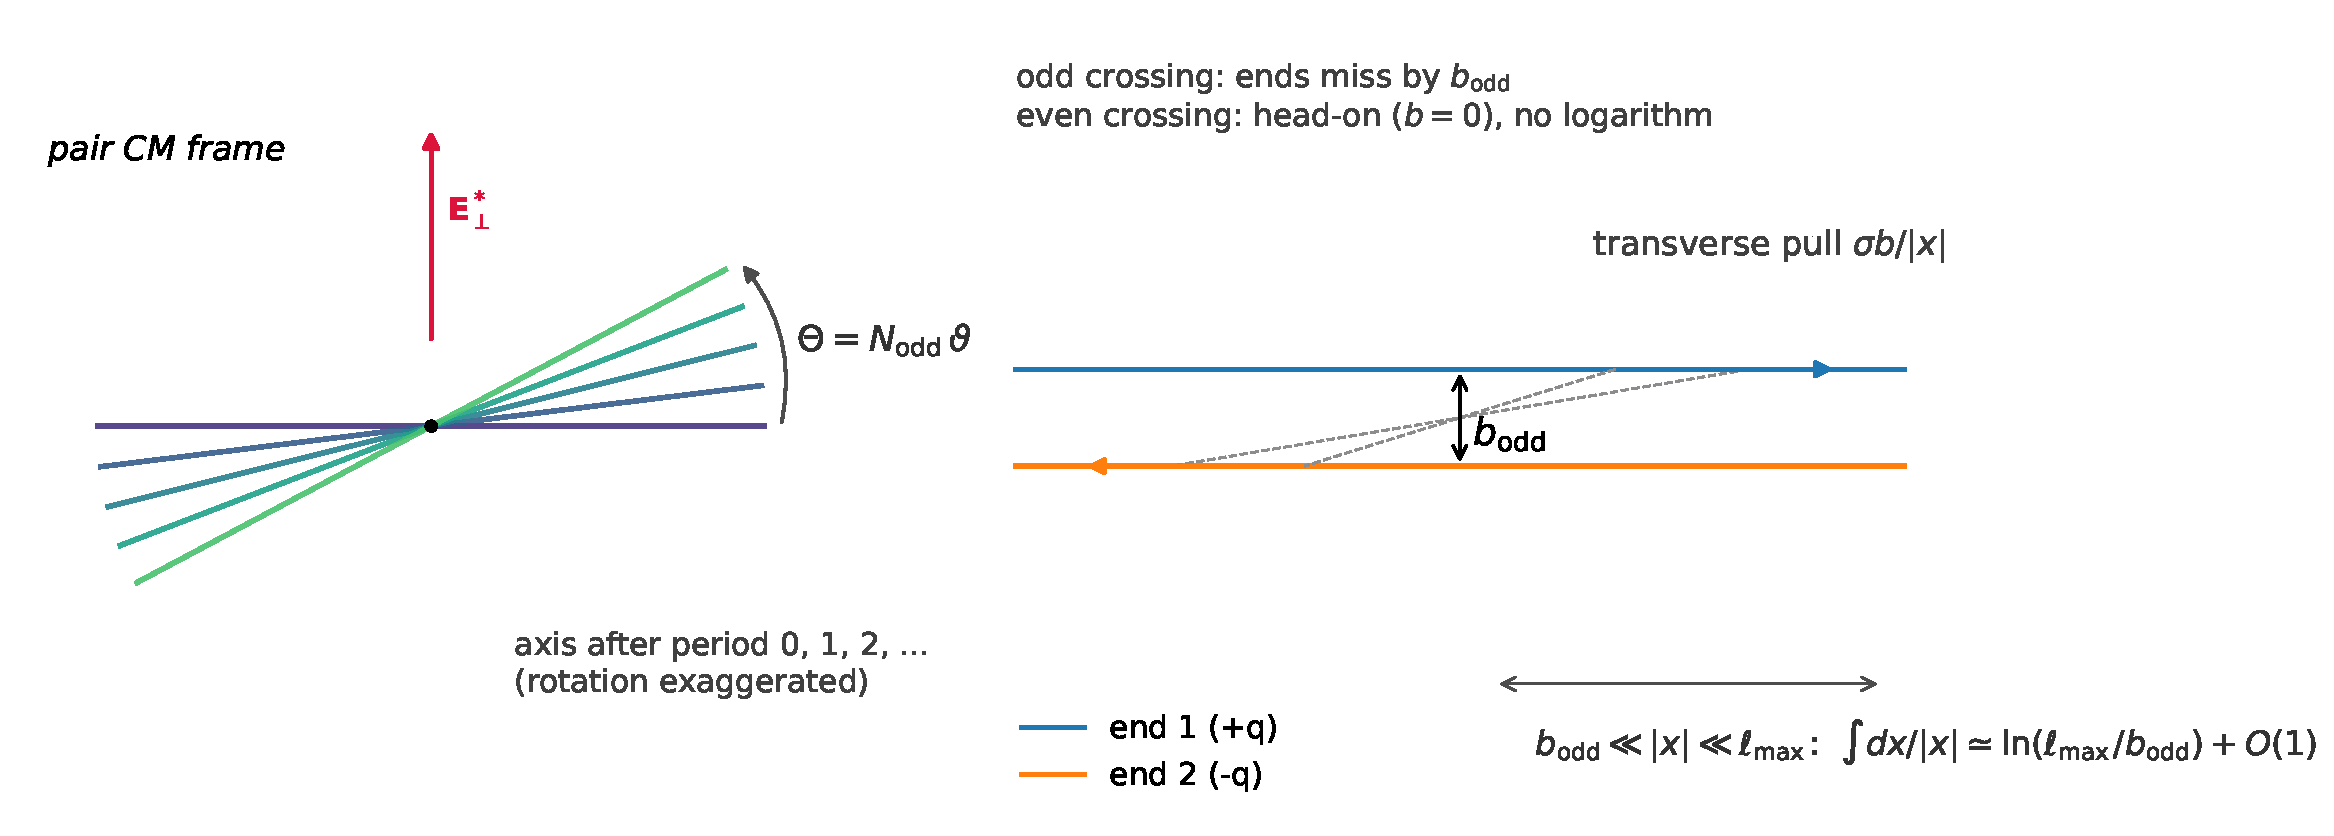
\includegraphics[width=0.92\linewidth,height=0.40\linewidth]{figures/schematic_nearmiss.pdf}
\caption{Schematic of the near-miss mechanism in the pair CM frame (conceptual diagram, not data; all scales
exaggerated). (Left) The oscillation axis turns by $\rot$ per period toward $\Estar_\perp$, coherently, so the rotation
accumulates as $\Theta=N_{\rm odd}\rot$. (Right) At an odd crossing the ends miss by $\bodd$, Eq.~\eqref{eq:bodd}; in
the region $\bodd\ll|x|\ll\lmax$ the string pulls the ends sideways with $\sigma\bodd/|x|$, whose integral gives the
logarithm of Eq.~\eqref{eq:rot}. Even crossings are head-on and carry no logarithm.}
\label{fig:schematic}
\end{figure}

\subsection{The per-period axis rotation}\label{sec:string:rot}
For a pure CM electric field ($\kB=0$) the rotation of the axis per CM period is
\begin{equation}
  \rot=\epsp\,G(\gst)\left[\ln\frac{\lmax}{\bodd}+K(\gst)\right],\qquad
  G(\gst)=\frac{2\left[\gst-\operatorname{asinh}(\gst\bst)/(\gst\bst)\right]}{\gst\bst\operatorname{artanh}\bst},
  \label{eq:rot}
\end{equation}
always toward $+\Estar_\perp$ and coherent from period to period, so that after $N_{\rm odd}$ odd crossings (one per period) the accumulated rotation is
$\Theta=N_{\rm odd}\rot$. The structure and $G$ are
derived; $G\to4/3$ in the non-relativistic limit, and $G=1.316/1.245/1.087/0.953$ at $\gst=1.05/1.28/2/3$. The slope of
$\rot/\epsp$ against $\ln(1/\epsp)$ in exact-NG numerics equals $G$ to 0.1--0.2\% at every $\gst$, which confirms the
retardation factor (the quasi-static $1/\bst$ would give slopes 1.03--1.87 times larger). The constant $K$ is analytic
only for slow ends, where a matched inner/outer calculation gives
\begin{equation}
  \rot_{\rm NR}=\tfrac43\,\epsp\left[\ln\frac{\lmax}{\bodd}+3\ln2-2\right],
  \label{eq:rotNR}
\end{equation}
i.e.\ $K(1)=3\ln2-2=0.0794$; at relativistic $\gst$ it is numerical (\EST{}, two solvers at $\gst=1.3$ and 2):
$K=+0.056/-0.049/-0.175/-0.309/-0.569$ at $\gst=1.05/1.28/1.6/2/3$, interpolated by
$K\simeq(3\ln2-2)-0.506\ln\gst-0.077\ln^2\gst$. Since $|K|\le0.6$ against $\ln(\lmax/\bodd)\approx8$--14, $K$ changes
the slope $c$ by at most 6\%.

\paragraph{Credit.} Li et al.\ observed that after each period the quirk system is rotated by a small angle (their
$\eta$), whose secular accumulation enters their thickness formula~\cite[Eqs.~(A.6), (A.17), (V.5)--(V.6),
(B.9)]{Li:2020aoq}; they determined it numerically and estimated $r|\eta|\sim d_E$. Equation~\eqref{eq:rot} is an
analytic expression for that angle. The logarithm itself is the elementary deflection of a nearly radial orbit passing a
constant-magnitude central force at impact parameter $b$; it is not a retardation or string-curvature effect, and a
step-converged straight-string integration has it too (Section~\ref{sec:string:valid}). Knapen et al.'s torque estimate
captures the scale $q|\Estar|/\sigma$ and the alternating half-period rotation~\cite[Eqs.~(8)--(9)]{Knapen:2017kly}, but
not the logarithmic secular term.

\subsection{The thickness law and the local slope $c$}\label{sec:string:law}
The plane fit sees only the component of the accumulated rotation out of the initial plane. Over the tracker the number
of periods scales as $\sigma$, the lever arm as $\lzero$, and $\rot\propto\epsp\propto qB/\sigma$, so the accumulated
tilt is $\sim qBR\,G[\ln(\lmax/\bodd)+K]/p^*$, a bending angle of momentum $p^*$ over $R$; the out-of-plane
displacement is this tilt times the lever arm $\sim\lzero\propto\mQ/\sigma$, i.e.\ $\propto qBR/\sigma=\epsB R$. With a
rotating-yo-yo model (the exact vacuum yo-yo whose axis steps by $\rot$ at each odd crossing, boosted to the lab; nothing
fitted) this gives
\begin{equation}
  \DsB=\frac{qBR}{\sigma}\,F\left[\ln\frac{1}{\epsB}+C\right],\qquad
  c\equiv\frac{d\ln(\DsB/\epsB)}{d\ln(1/B)}=\frac{1}{\ln(1/\epsB)+C},
  \label{eq:law}
\end{equation}
where $F$ is a dimensionless function of the CM velocities, angles and layer phases, independent of $\mQ$ and $\Lam$ at
fixed velocities, and $C=-\ln(\gamma_{\rm cm}\beta_{T,\rm cm}\sin\alpha)+\ln[(\gst-1)/(\gst-\operatorname{asinh}(\gst\bst)
/(\gst\bst))]+K(\gst)$ collects the event kinematics ($\alpha$ is the CM angle between $\Estar$ and $\hat n$). The model
population values are $C=0.43/1.23/1.62$ at $\mQ=200/500/1000\GeV$; Eq.~\eqref{eq:law} then predicts local exponents
\begin{equation}
  \frac{d\ln\DsB}{d\ln B}=1-c,\qquad \frac{d\ln\DsB}{d\ln\Lam}=-2+2c,\qquad \mathcal R(f)\equiv\frac{\DsB(fB)}{f\,\DsB(B)}=1+c\ln\frac1f .
  \label{eq:exponents}
\end{equation}
Limiting cases: for $B\to0$, $\DsB/B\propto\ln(1/B)$ (non-analytic); for $\alpha=0$ ($\Estar\parallel\hat n$) the
rotation vanishes. The model accuracy against the exact causal string, event by event, is 1--4\% (median) for
$\gst\lesssim1.6$, which covers 84--97\% of events at $500$--$1000\GeV$ and 66\% at $200\GeV$; it is 10--35\% off for
$\gst>2$ (16\% of events at $200\GeV$, 7\% at $500\GeV$), where the rotation is spread over the half period and the CM
magnetic field acts (\EST{}).

Table~\ref{tab:c} gives the predicted population medians of $c$. The predicted fall of $c$ with $\Lam$ (0.116 to 0.070
from 0.6 to $10\keV$ at $500\GeV$) is the main test of Eq.~\eqref{eq:law}. In terms of scaling, $\DsB\approx
\Lam^{-1.8}B^{0.9}$ and is flat in $\mQ$ within errors: the model medians are $33.5/31.1/29.5\um$ at
$200/500/1000\GeV$ and $1\keV$, because the $\mQ$ dependence of $C$ and of the $\gst$ spectrum compensate. The
$\mQ$-independent $B/\Lam^2$ scaling of the plane rotation was estimated by Knapen et
al.~\cite[Eqs.~(8)--(9)]{Knapen:2017kly}, and Li et al.\ found a mild $\mQ$ and $p_T$ dependence
numerically~\cite[Sec.~V, Fig.~4]{Li:2020aoq} (also Ref.~\cite[Fig.~4]{Li:2019wce}: the confinement-scale
dependence is much stronger than the mass dependence); what is new here is the logarithm, the exponents' departure from
$\Lam^{-2}B$, and the constants.\footnote{The form $\DsB\propto\epsB[1+c\ln(\Lam^2/qB)]$ with a constant $c$ is not
equivalent to Eq.~\eqref{eq:law}: it predicts a $B$ exponent of 0.944 instead of the measured 0.911.}

\begin{table}[htbp]
\centering
\caption{Predicted population median of the local slope $c$ of Eq.~\eqref{eq:law} (16--84\% range in parentheses),
rotating-yo-yo model on the project's truth-level event sample, $B_0=3.8112\tesla$, $|\eta_{\rm pair}|<1$ (Stage-1
note \S5.3, \rep{analytic/predictions.json}). The $1\keV$, $500\GeV$ entry is verified by blind numerics,
$0.105\pm0.002$ (Table~\ref{tab:numerics}).}
\label{tab:c}
\begin{tabular}{rcccccc}
\toprule
$\mQ$ [GeV] & $0.6\keV$ & $1\keV$ & $2\keV$ & $3\keV$ & $5\keV$ & $10\keV$\\
\midrule
200  & 0.128 & 0.113 (0.108--0.120) & 0.098 & 0.091 & 0.083 & 0.074\\
500  & 0.116 & \textbf{0.104} (0.098--0.112) & 0.091 & 0.085 & 0.078 & 0.070\\
1000 & 0.111 & 0.100 (0.095--0.107) & 0.088 & 0.082 & 0.076 & 0.068\\
\bottomrule
\end{tabular}
\end{table}

\subsection{Numerical verification}\label{sec:string:numerics}
The predictions were tested by an independent ``blind'' numerics campaign that did not see the analytic coefficients
before finishing (\rep{analytic/numerics/NUMERICS.md}). The production solver is a causal, piecewise-null NG string
(the construction of Artru and of the Lund model~\cite{Artru:1979ye,Andersson:1983ia}; for segmented strings see also
Ref.~\cite{Gubser:2016wno}), as implemented for quirks in the ATLAS Athena Geant4 extension (software path
\rep{Simulation/G4Extensions/Quirks}) by J.~Black and T.~Nelson and used by FASER~\cite[App.~A]{FASER:2026fsy}; the second solver is a
conformal-gauge delay ODE with a different formulation and arithmetic. Table~\ref{tab:numerics} compares the headline
numbers. Per crossing, the miss distance matches Eq.~\eqref{eq:bodd} to $10^{-4}$ in controlled CM-frame runs and to
0.6--2\% in full events; the per-crossing rotation matches the vacuum law to 1--2\%.

\begin{table}[htbp]
\centering
\small
\caption{Predictions of Section~\ref{sec:string} against blind numerics (truth level, field only, no material; Stage-1
note \S5.3, \S9; \rep{NUMERICS.md} \S0, \S4). $\mathcal R(f)$ is the response per unit field of Eq.~\eqref{eq:exponents} at
$\mQ=500\GeV$, $\Lam=1\keV$. ``Two solvers'' means causal and conformal codes agree.}
\label{tab:numerics}
\begin{tabularx}{\linewidth}{>{\raggedright\arraybackslash}Xccl}
\toprule
quantity & prediction & numerics & status\\
\midrule
$\bodd/(\epsp\lmax)$ at $\gst=1.05/1.3/2/3$ & 1.327/1.298/1.240/1.188 & 1.328/1.298/1.240/1.189 & two solvers\\
$c$ ($500\GeV$, $1\keV$) & 0.104 & $0.105\pm0.002$ & verified\\
$B$ exponent over $B_0/80\ldots B_0$ & 0.914 & $0.911\pm0.003$ & verified\\
$\mathcal R(1/2,1/4,1/20,1/80)$ & 1.072/1.144/1.311/1.455 & 1.073/1.147/1.320/1.460 & $\pm0.001$--0.005\\
$|q|=2$: $\DsB(2B_0)/\DsB(B_0)$ & $2[1-c\ln2]$ & ratio to pred.\ $0.999\pm0.001$ & verified\\
$K_{\rm vac}$ (non-relativistic) & $3\ln2-2=0.0794$ & $0.0791\pm0.0003$ & two solvers\\
\bottomrule
\end{tabularx}
\end{table}

\subsection{Validity, open terms and a failed prediction}\label{sec:string:valid}
\paragraph{The CM magnetic field.} In linear response $\Bstar$ neither changes $\bodd$ nor rotates the axis (its forces on
the two ends are odd under exchange), but it enters the non-linear inner region of the odd crossing. Measured in exact
NG runs, its effect on $\rot$ is even in $\Bstar$, vanishes for $\gst\to1$, is non-monotonic in $\kB$ and reaches
$-7$ to $-21\%$ at $\gst=2$ for $\kB=4$--16 (\EST{}; mechanism conjectural). Per event, $c$ shifts by $+17$ to $+36\%$
for $\kB=8$--12; events with $\kB>6$ are 5/29/43\% of the sample at $200/500/1000\GeV$, for which the per-event $c$ is
not reliable. \paragraph{Population-level status of $c$ (used throughout this note).} The prediction for the population median of
$c$ is confirmed by the blind numerics at $1\keV$ within $1.5\%$ ($0.105\pm0.002$ against 0.104,
Table~\ref{tab:numerics}). On the full-kinematics Stage-3 simulation (Section~\ref{sec:p1:law}) the per-event law
holds (paired agreement $\le1\%$ at $1\keV$), but the population median of the measured $c$ lies $+2$--$3\%$ above the
prediction at $1\keV$ ($+2.0/+2.1/+3.2\%$ at $E$ 500/$E$ 1500/$\Etil$ 500; $+0.7/+1.1\%$ at $E$ 200/1000), failing
the pre-set $1.5\%$ validation gate; pooled over $1$--$2\keV$ the excess is $+1.71\pm0.29\%$, which a zero-median
symmetric per-event scatter reproduces ($+2.04\%$), so we read it as an estimator effect (\EST{}). The population
uncertainty on $c$ at $1$--$2\keV$ is therefore quoted as $+2$--$3\%$; at $3$--$5\keV$ a larger, $\kB$-dependent excess
is attributed to $\Bstar$ (\EST{}, Section~\ref{sec:p1:law}).

\paragraph{Scale-free equivalence and the high-$\Lam$ systematic.} Scaling all coordinates by $\lambda$ maps a solution
for $(\sigma,qB)$ onto one for $(\sigma/\lambda,qB/\lambda)$: per oscillation $(\Lam\sqrt k,B)$ is the same physics as
$(\Lam,B/k)$, with $\Nosc$ larger by $k$. The law is verified at $\Lam\approx1\keV$ (blind numerics: population $c$ within
$1.5\%$, $C$ to 0.1--0.2; full simulation: $+2$--$3\%$, see above), consistent at $3$--$5\keV$ ($\lesssim1\%$ on $\DsB(5)/\DsB(3)$), and not verified above $\approx5\keV$, where
an excess seen in weak-field scans combines a cumulative $\Bstar$ part with a double-precision floor of both solvers
($\bodd/\lzero\approx3\times10^{-8}$). An unmeasured, unattributed systematic of order $\pm5\%$ on $\DsB$ (population;
sign expected positive) and up to tens of per cent on the per-event $c$ for $\kB\gtrsim10$ is therefore carried above
$5\keV$. Two decisive floor tests (extended precision on a scaled detector; reduced-precision emulation) are specified but
were not run.

\paragraph{Classical validity.} Classical NG holds at odd crossings while $\bodd\gg1/\Lam$, i.e.\ for $\Lam\lesssim10\keV$
for all events and up to $\Lam\approx26\keV$ for typical ones; beyond, the lower cut-off of the logarithm becomes $\sim1/\Lam$
and the model uncertainty on $\DsB$ is $\approx3$--8\% at $30\keV$ (\EST{}). Above $\Lcross\approx1.2$--$1.9\keV$ (depending on $\mQ$)
$\DsB$ is below the multiple-scattering floor anyway (Section~\ref{sec:p1:ms}).

\paragraph{Charge and spin.} Since $q$ enters only through $qB$, $\DsB(q)/\DsB(1)=q[1-\ln q/(\ln(1/\epsB)+C)]$, i.e.\
1.86 rather than 2 for $|q|=2$ (verified numerically, Table~\ref{tab:numerics}). This implies a $\approx c\ln2\approx7\%$
deviation from linearity in Li et al.'s factor-two charge test, consistent with their ``linearly proportional'' at their
precision~\cite[Sec.~V.A, Fig.~4]{Li:2020aoq}. Classical NG has no spin: for the scalar the per-event law is the same and
only the $\gst$ spectrum changes (median $\gst=1.39$ vs 1.23 at $500\GeV$), which roughly doubles the model uncertainty
(\EST{}).

\paragraph{Straight strings and a failed prediction.} Any attraction of fixed magnitude along the string gives
$\sigma b/|x|$ and hence the logarithm, so a step-converged straight-string (``Li-method'') integrator~\cite{Li:2019wce,Li:2020aoq}
also shows the $B\ln(1/B)$ response: its $c$ agrees with NG within $\approx3\%$ at $\gst=1.28$. The size of the
rotation differs, however, and the predicted straight-string/NG thickness ratio at $\gst=2$, 0.50, \textbf{fails}: the
measurement is $0.75\pm0.08$ (30 events; a 10-event subset at a finer step gives $0.96\pm0.10$), a $\approx3\sigma$
discrepancy. Three candidate causes ($\Bstar$ in the exact string, the breakdown of $\DsB\propto\rot$ at $\gst=2$, and a
frame-dependent miss-distance ratio) are identified but not quantified; the structural statements above are unaffected.
This answers the call for a direct check of the straight-string approximation~\cite[Sec.~3.2]{Kang:2008ea} and the
neglect of retardation in Ref.~\cite[Sec.~2]{Evans:2018jmd} at the level of a direct comparison, without implying an
error in published limits, which use the numerical thickness within an order of magnitude~\cite[App.~C]{Li:2020aoq}.

\paragraph{Scope.} By user decision, P1 is restricted to the B-field crossing physics: multiple scattering enters only as
the measured floor of Section~\ref{sec:p1}, with the Highland $\sqrt{x/X_0}$ scaling~\cite{Highland:1975pq,ParticleDataGroup:2024cfk}
credited, and no analytic multiple-scattering claim is made. Material-induced rotations of the quirk plane were estimated
and neglected by Knapen et al.~\cite[Sec.~II]{Knapen:2017kly} and studied for ionisation in the FASER geometry by Li et
al.~\cite[Sec.~4.1]{Li:2021tsy}. Classical strings with massive charged ends in constant fields were previously solved
only for motions linear in the endpoint proper time~\cite{Barbashov:1977tv}, which in 3+1 dimensions reduce to uniform
rotations~\cite{Petrov:1996wz}; the field-driven yo-yo with a near miss is outside that class.

\section{Truth-level propagation and P1 results}\label{sec:p1}

The thickness law of Section~\ref{sec:string} was derived and checked on small controlled samples. This section tests it
on the full Stage-2 kinematics with $2.2\times10^5$ propagated events and compares the B-field thickness with the
multiple-scattering (MS) floor. Everything here is \textbf{truth level}: true hit positions, known hit-to-quirk assignment,
no pile-up, no resolution. Full detail is in \rep{sim/stage3/README.md} and \rep{sim/stage3/VALIDATION.md}; the numbers
are taken from \rep{sim/stage3/results/P1.json}.

\subsection{Propagation}\label{sec:p1:prop}
The Stage-3 kernel is the causal piecewise-null NG propagator of Section~\ref{sec:string:numerics} extended with
material effects: Bethe ionisation loss with straggling, Highland multiple scattering~\cite{Highland:1975pq} and the
magnetic kick, applied to each end; it reproduces the Stage-1 kernel bit for bit with material switched off. Hits are
recorded on 93 surfaces of a public CMS Phase-2 tracker layout (the tkLayout D111 configuration underlying
Ref.~\cite{CMS:2017lum}): the barrel and endcap Inner Tracker (IT), the stacked PS and 2S modules of the Outer Tracker
(OT), the barrel timing layer and ten virtual barrel layers for the P1 observable. The material is a per-layer slab of
1.2\% $X_0$ (IT barrel), 2.5\% (PS), 1.8\% (2S), 0.23\% for the beryllium beam pipe and 1.0\% for the IT service
cylinder (\UNV{}; varied by $\times0.5$ and $\times2$). The step parameter is $10^{-3}$ for field-only runs (at $10^{-2}$, $\DsB$ would be biased
by $+0.1$ to $+1.6\%$) and $10^{-2}$ with material. At $10^{-2}$ the out-of-plane hit displacement (median of the
per-event maximum) is 0.2--4$\um$ at $0.3$--$1\keV$ and $\le0.3\um$ at $2$--$3\keV$; the step-convergence test V3 (30
of 32 cells pass) covered field-only configurations. The material runs at $0.45$--$1.5\keV$ were not tested separately:
their field part carries up to $+1.6\%$ step bias, small against the multiple-scattering floor and the 3--20\% dip of
Section~\ref{sec:p1:ms}, and in the direction of quadrature, i.e.\ conservative for the dip (\EST{}).

The production comprised 4576 jobs and $218\,571$ events ($1.27\times10^7$ hits), split between two machines whose
kernel output is bit-identical in 224 of 225 overlap events (the exception differs by $4.4\um$). The P1 grid uses the
fermion at $\mQ=200,500,1000,1500\GeV$ and the scalar at $500\GeV$, $\Lam=0.45$--$10\keV$, $|\eta_{\rm pair}|<1$, the
vertex at the origin and 300 events per point (200 at 7 and $10\keV$). The same events are propagated in several
configurations: field only at $B_0$ and $B_0/2$ (giving $\DsB$ and, per event, $c=[\mathcal R(1/2)-1]/\ln2$), material only
($\DsMS$), field and material ($\DsBM$), the vacuum (a $\Ds\equiv0$ check) and the material variations.

\subsection{B-field thickness against the law}\label{sec:p1:law}
Figure~\ref{fig:p1law} and Table~\ref{tab:p1} compare the measured $\DsB$ and $c$ with the rotating-yo-yo model
evaluated on the same events. The primary statistic is the paired per-event ratio of measured to model thickness.
\begin{itemize}
\item \textbf{Thickness.} The paired median ratio is 0.990--1.002 for the fermion at $\mQ\ge500\GeV$ and
  $0.6$--$5\keV$, 0.966--0.990 at $200\GeV$ and 0.947--0.986 for the scalar: the model agrees per event to $\le3.4\%$
  (fermion) and $\le5.3\%$ (scalar), inside its declared 1--4\% accuracy for the fermion. The deviation is driven by
  $\gst$, not by spin: the ratio is within 0.8\% of one for $\gst<1.3$, 0.96--0.98 at $\gst=1.3$--1.6 and 0.89--0.93
  above. $\DsB$ is flat in $\mQ$ ($d\ln\DsB/d\ln\mQ=-0.004\ldots-0.07$ for $0.45$--$5\keV$).
\item \textbf{The $c$ law.} Per event, the law holds: in the pre-registered gate sample the paired agreement is
  $\le1\%$ at $1\keV$, and in the full production the conditional median of $c$ agrees with the event's prediction
  within $\pm1.5\%$ at $1$--$2\keV$ (every $\kB$ bin within $\pm2.4\%$). \textbf{The population median does not pass
  the pre-set gate}: at $1\keV$ it lies $+0.7/+2.0/+1.1/+2.1/+3.2\%$ above the prediction for $E$ 200/500/1000/1500 and
  $\Etil$ 500 (2.2--2.4$\sigma$ at the three failing points), against a pre-declared limit of $1.5\%$ at all five points
  (gate V2b, \rep{sim/stage3/VALIDATION.md}); pooled over $1$--$2\keV$ the excess is $+1.71\pm0.29\%$, and the same
  number appears in $\mathcal R(1/2)=1.0737\pm0.0007$ at $500\GeV$ (2.4$\sigma$ above 1.072). A zero-median symmetric
  per-event scatter reproduces it ($+2.04\%$), so we read it as an estimator effect (\EST{}); it is not a step effect.
  The user decided to proceed past the gate and to record it as a finding (\rep{LOG.md}, 2026-10-11). In dimensionless terms the law holds for median
  $\lmax/\RIT\lesssim0.6$ and $\kB\lesssim4$, with $\RIT\approx14.6\cm$ the outer IT barrel radius. At $0.45\keV$ it fails
  ($\kB$-ordered residuals from $+6\%$ to $-26\%$), where the non-secular $\Lam^{-4}$ terms omitted in the model matter
  and the pair does not turn around inside the IT. The $\Lam$ exponent $-2+2c$ is the asymptotic one ($\lmax\ll\RIT$). The measured slopes are steeper by
  3.9--5.9$\sigma$ for $0.6\to1\keV$ at all five points, by 4.1/4.5$\sigma$ for $1\to2\keV$ at $E$ 1500/$\Etil$ 500 and by
  3.0/3.4/3.9$\sigma$ for $1\to3\keV$ at $E$ 1000/$E$ 1500/$\Etil$ 500, i.e.\ wherever $\lmax/\RIT$ at the lower end
  reaches $\approx0.5$--0.6 (Table~\ref{tab:p1}); the edge of the validity window is therefore soft. The full
  event-level model agrees in every interval ($|{\rm pull}|\le2.6$).
\item \textbf{The $3$--$5\keV$ excess.} At $3$--$5\keV$ events with large $\kB$ carry a positive excess of $c$ whose size is
  measured: up to $+57\pm11\%$ at $5\keV$ for $\kB\ge10$ and $+3$ to $+5\%$ already at $\kB<4$; the population-median
  excess is $+6.2\pm0.5\%$. Its \textbf{attribution to the CM magnetic field is an estimate}: it grows with $\Nosc$ at matched
  $\kB$ and $\epsp$, and switching $\Bstar$ off in a dedicated run (160 events at $500$ and $1000\GeV$) removes the bulk
  of the population-median excess ($+1.8\pm0.7\%$ against $+9.7\pm1.3\%$ for the same masses, $5.5\sigma$; paired on the
  same events the difference is $+8.6\pm4.2\%$). With $\Bstar$ off, the residual is $\le3\%$ for $\kB<10$ and $+12\pm3\%$
  at $\kB\ge10$, inside the allowance for the double-precision floor of Section~\ref{sec:string:valid}. \textbf{The floor
  test (O-1) that would separate the two was not done.}
\item \textbf{Above $5\keV$.} The paired ratio rises to $1.016\pm0.005$ ($500\GeV$) and $1.027\pm0.005$ ($1000\GeV$) at
  $10\keV$, not carried by floor-flagged events; this turns part of the unattributed $\pm5\%$ of
  Section~\ref{sec:string:valid} into a measured $+1.6\%/+2.7\%$, of the same sign as the $c$ excess.
\end{itemize}

\begin{figure}[htbp]
\centering
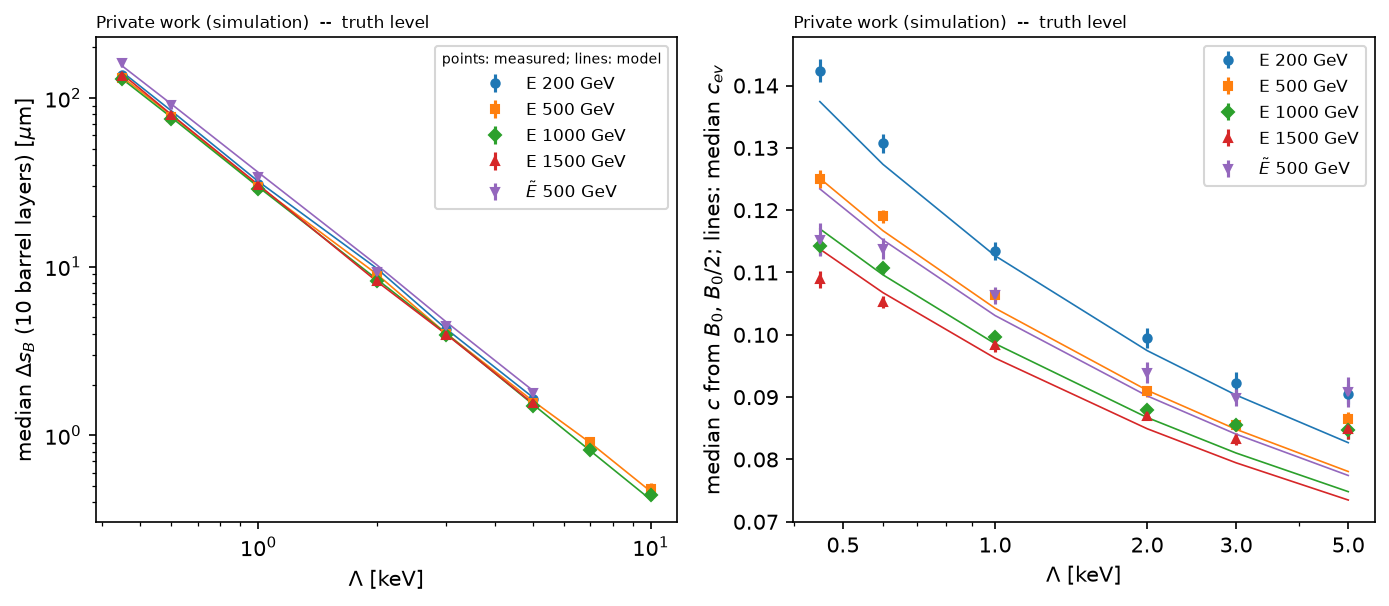
\includegraphics[width=0.98\linewidth,height=0.40\linewidth]{figures/S3_p1_dsB_c.png}
\caption{P1 at truth level (field only, no material, $|\eta_{\rm pair}|<1$, vertex at the origin, ten barrel layers;
Stage-3 diagnostic figure). (Left) Median B-field plane thickness $\DsB$ against $\Lam$ for the five (species, mass) points:
points are the propagation, lines the rotating-yo-yo model on the same events; the curves fall as $\approx\Lam^{-1.8}$
and are nearly independent of $\mQ$. (Right) Median local slope $c$ from paired $B_0$ and $B_0/2$ runs (points) and the
median per-event prediction $1/[\ln(1/\epsB)+C_{\rm ev}]$ (lines). The prediction is followed at $1$--$3\keV$; the
excess at $5\keV$ is the $\kB$-dependent effect discussed in the text, and the $0.45$--$0.6\keV$ deviations mark the
breakdown of the law where $\lmax$ approaches the IT radius.}
\label{fig:p1law}
\end{figure}

\begin{table}[htbp]
\centering
\footnotesize
\setlength{\tabcolsep}{4pt}
\caption{P1 at truth level at $\Lam=1$ and $5\keV$ (the $3\keV$ rows are in the source table) (Stage 3, \rep{sim/stage3/README.md} results table). ``ratio'' is the
paired per-event median $\DsB^{\rm meas}/\DsB^{\rm model}$ with its bootstrap error; $c$ is measured from $B_0$ and
$B_0/2$ and compared with the median per-event prediction $c_{\rm ev}$; $\DsMS$ is the material-only thickness and the
last column the measured $\DsBM/\sqrt{\DsB^2+\DsMS^2}$. Errors on $\DsB$ and $\DsMS$ are bootstrap errors of the median.}
\label{tab:p1}
\begin{tabular}{llccccccc}
\toprule
point & $\Lam$ & $\lmax/\RIT$ & $\DsB$ [$\mu$m] & ratio & $c$ (meas.) & $c_{\rm ev}$ & $\DsMS$ [$\mu$m] & BM\\
\midrule
$E$ 200  & 1 & 0.19  & $31.1\pm1.8$   & $0.986\pm0.001$ & $0.1135\pm0.0014$ & 0.1127 & $9.9\pm0.6$ & $0.97$\\
         & 5 & 0.0075& $1.64\pm0.09$  & $0.990\pm0.002$ & $0.0905\pm0.0016$ & 0.0827 & $11.3\pm0.6$ & $0.89$\\
$E$ 500  & 1 & 0.37  & $29.5\pm1.6$   & $0.993\pm0.001$ & $0.1064\pm0.0009$ & 0.1043 & $13.2\pm1.1$ & $0.94$\\
         & 5 & 0.015 & $1.56\pm0.08$  & $0.997\pm0.001$ & $0.0865\pm0.0011$ & 0.0781 & $15.5\pm1.0$ & $0.99$\\
$E$ 1000 & 1 & 0.52  & $28.7\pm1.5$   & $0.998\pm0.001$ & $0.0996\pm0.0008$ & 0.0986 & $18.2\pm1.2$ & $0.95$\\
         & 5 & 0.021 & $1.49\pm0.08$  & $1.000\pm0.001$ & $0.0848\pm0.0015$ & 0.0748 & $22.3\pm1.5$ & $0.93$\\
$E$ 1500 & 1 & 0.61  & $30.4\pm1.1$   & $0.999\pm0.001$ & $0.0983\pm0.0010$ & 0.0963 & $22.8\pm1.5$ & $0.93$\\
         & 5 & 0.024 & $1.56\pm0.05$  & $1.002\pm0.000$ & $0.0848\pm0.0016$ & 0.0735 & $24.5\pm2.0$ & $1.09$\\
$\Etil$ 500 & 1 & 0.59 & $33.9\pm2.3$ & $0.969\pm0.005$ & $0.1063\pm0.0014$ & 0.1031 & $14.5\pm1.3$ & $0.95$\\
         & 5 & 0.024 & $1.79\pm0.12$  & $0.952\pm0.008$ & $0.0908\pm0.0024$ & 0.0774 & $14.3\pm0.9$ & $1.03$\\
\bottomrule
\end{tabular}
\end{table}

\subsection{The multiple-scattering floor and the combination of B and MS}\label{sec:p1:ms}
With material, the plane thickness has a floor that is nearly independent of $\Lam$: the median $\DsMS$ is $\approx10$,
13--16, 17--22, 18--28 and 12--16$\um$ for $E$ at $200/500/1000/1500\GeV$ and $\Etil$ at $500\GeV$ (truth level,
nominal material). It rises with $\mQ$ because heavier pairs are slower and scatter more. The material scaling exponents
$\ln[\DsMS(\times2)/\DsMS(\times0.5)]/\ln4$ are 0.36--0.62, against $\approx0.5$ expected from the Highland $\sqrt{x/X_0}$
scaling~\cite{Highland:1975pq,ParticleDataGroup:2024cfk} ($\chi^2=26.0/10$ against the single-point code-scaling value
0.517; the $1000$ and $1500\GeV$ points are low by 2--2.6$\sigma$). The crossover $\DsB=\DsMS$ falls with mass:
$\Lcross=1.91/1.50/1.25/1.16\keV$ for $E$ at $200/500/1000/1500\GeV$ and $1.59\keV$ for $\Etil$. Above $\Lcross$ the
coplanarity of a truth-level quirk pattern is limited by material, not by the field.

Figures~\ref{fig:u2} and~\ref{fig:u2ratio} show how the two effects combine. Per event they add
\emph{below quadrature} in the crossover region: the median of $\DsBM/\sqrt{\DsB^2+\DsMS^2}$ is 0.99--1.00 at $0.45\keV$,
0.95--1.00 at $0.6\keV$ and 0.80--0.97 at $1$--$3\keV$ (lowest: $E$ 200 at $3\keV$, $0.804\pm0.042$), and consistent with
one within $2\sigma$ at $5$--$10\keV$; the dip is deepest at $\Lam/\Lcross=1.25$--1.73. The ratio to the linear sum is
0.62--1.00. No combination rule is fitted; the measured ratios are reported as they are (user decision, Appendix~\ref{app:limits}).

\begin{figure}[htbp]
\centering
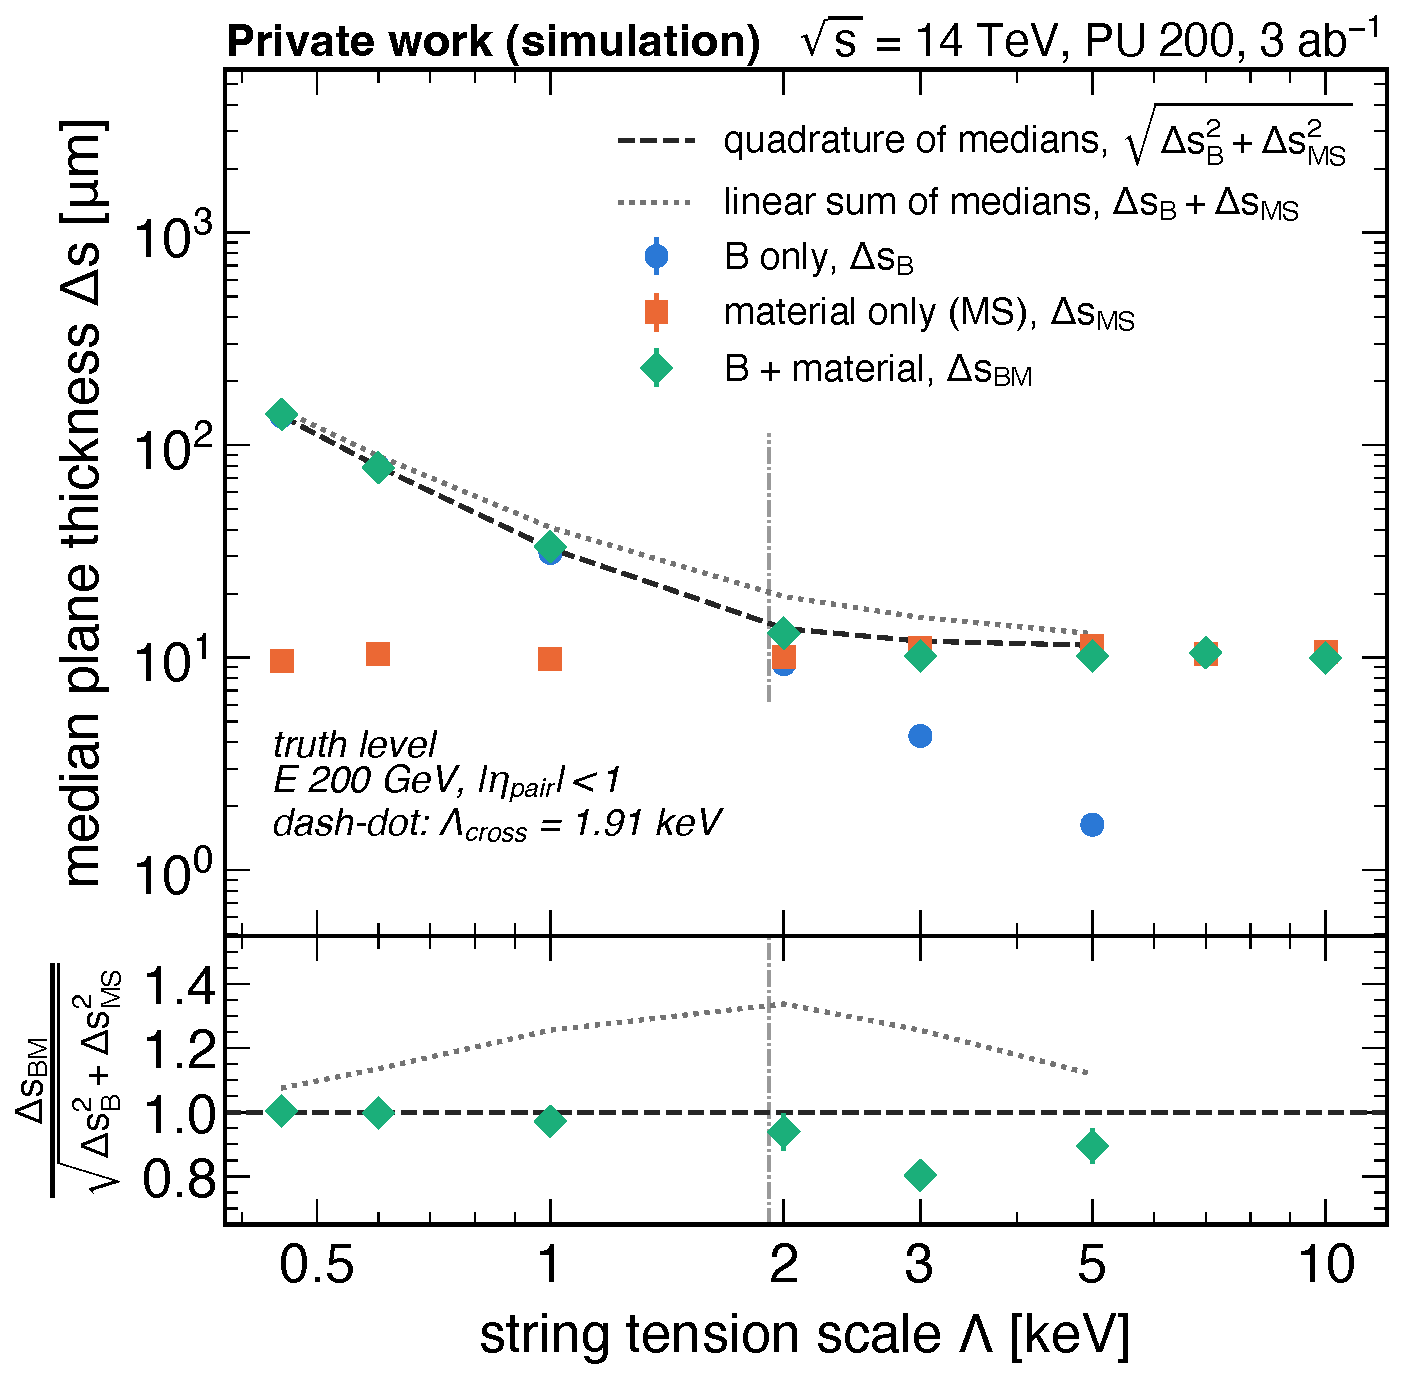
\includegraphics[height=0.34\linewidth]{figures/T1_u2_thickness_F_m200.pdf}\hspace{0.02\linewidth}
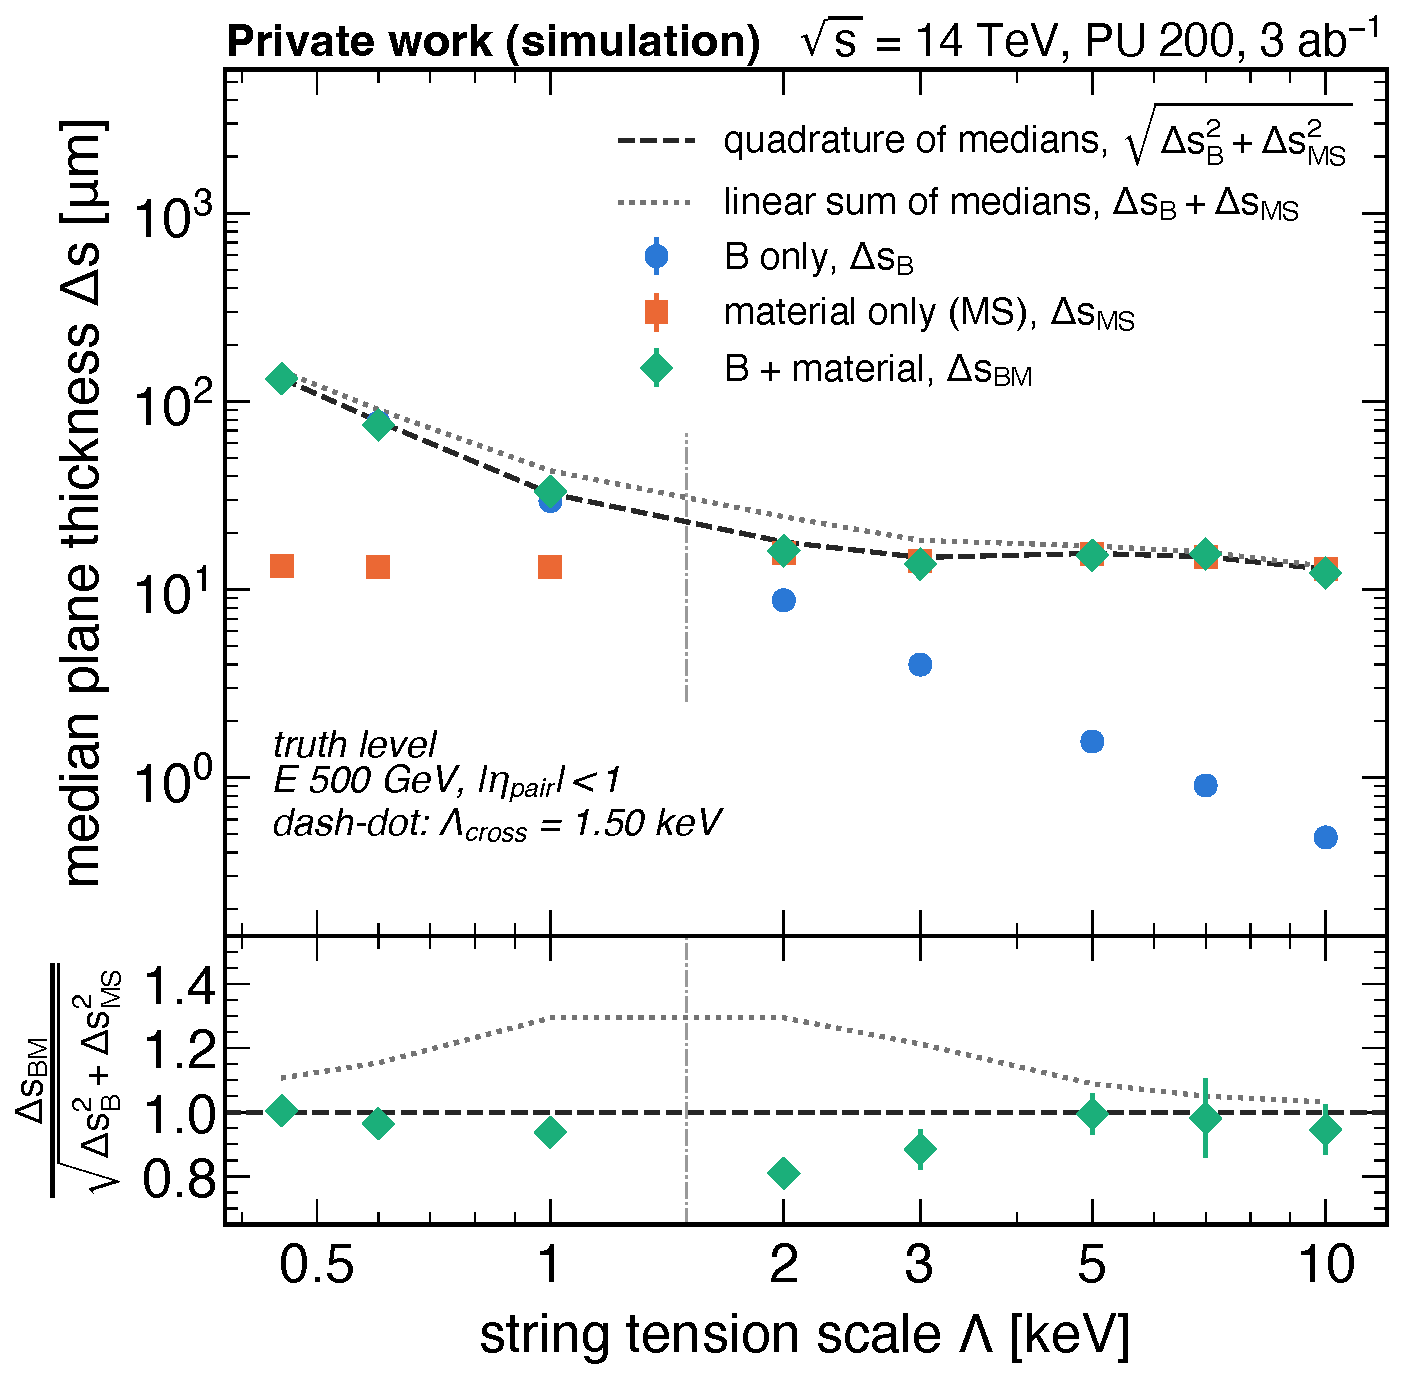
\includegraphics[height=0.34\linewidth]{figures/T1_u2_thickness_F_m500.pdf}\\[4pt]
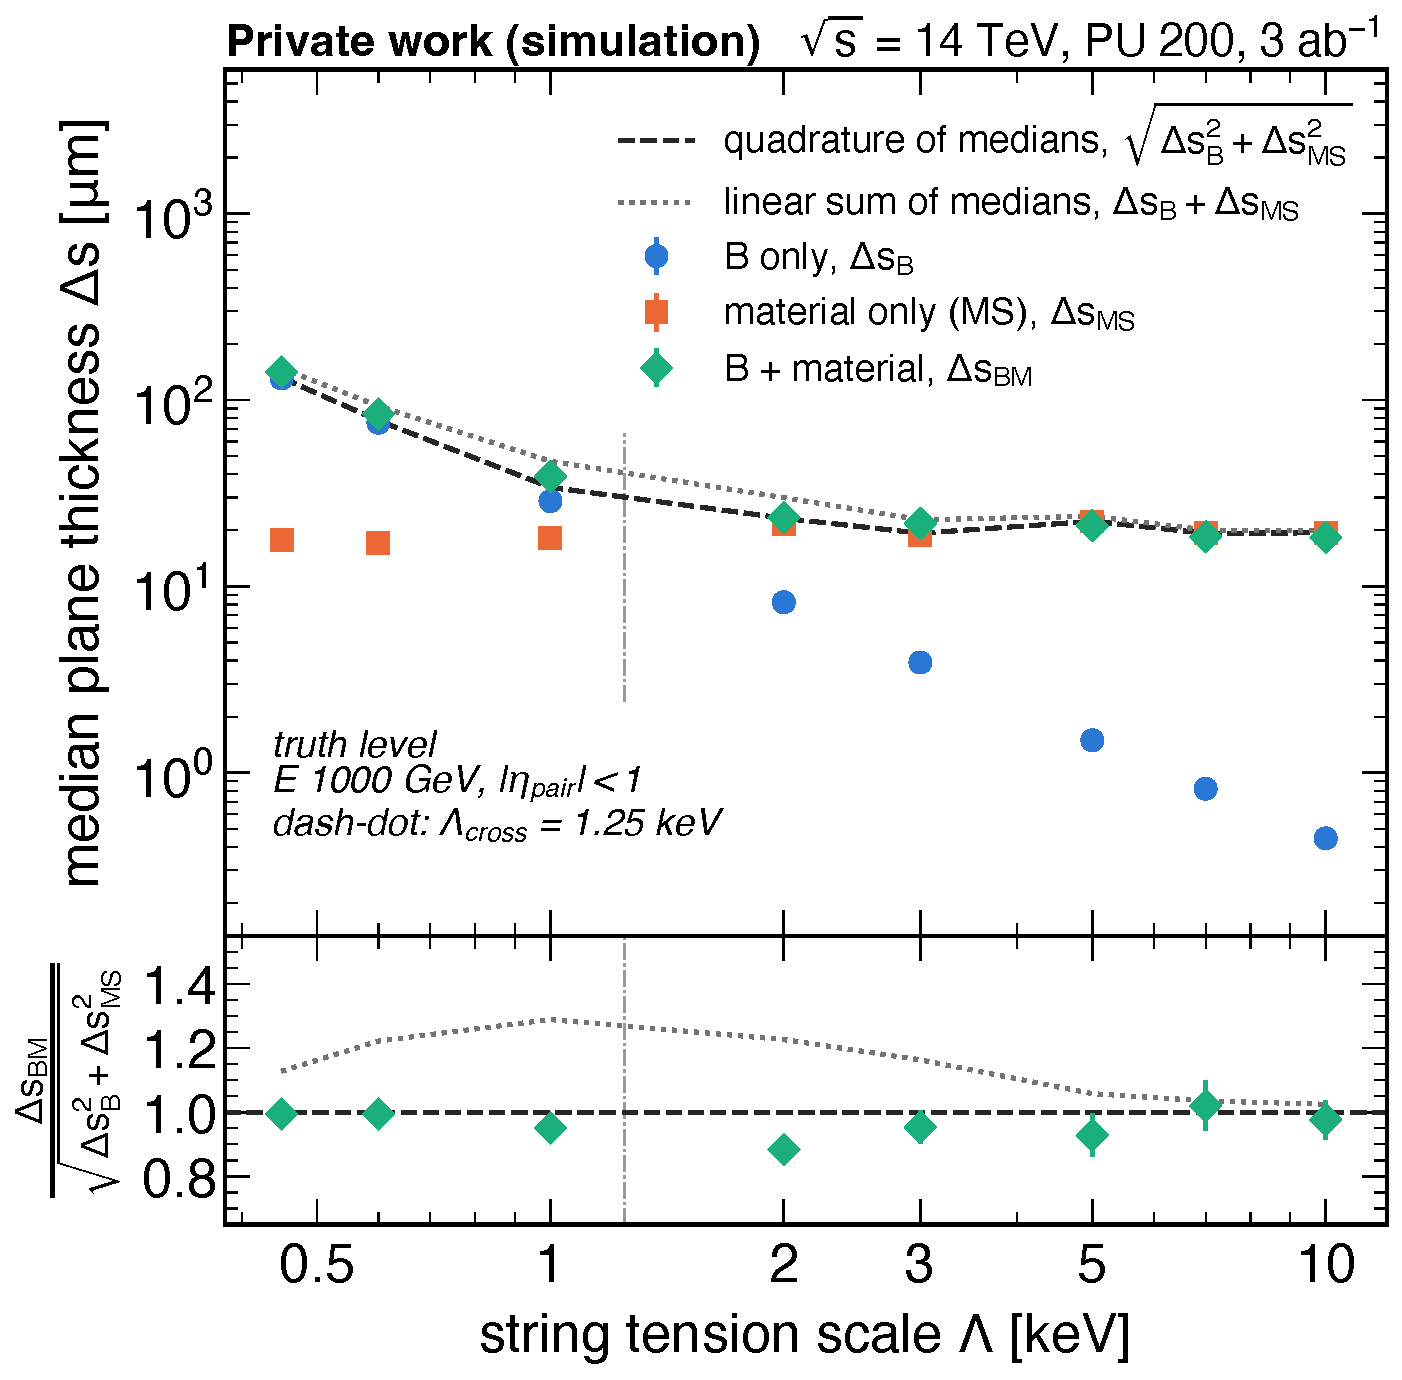
\includegraphics[height=0.34\linewidth]{figures/T1_u2_thickness_F_m1000.pdf}\hspace{0.02\linewidth}
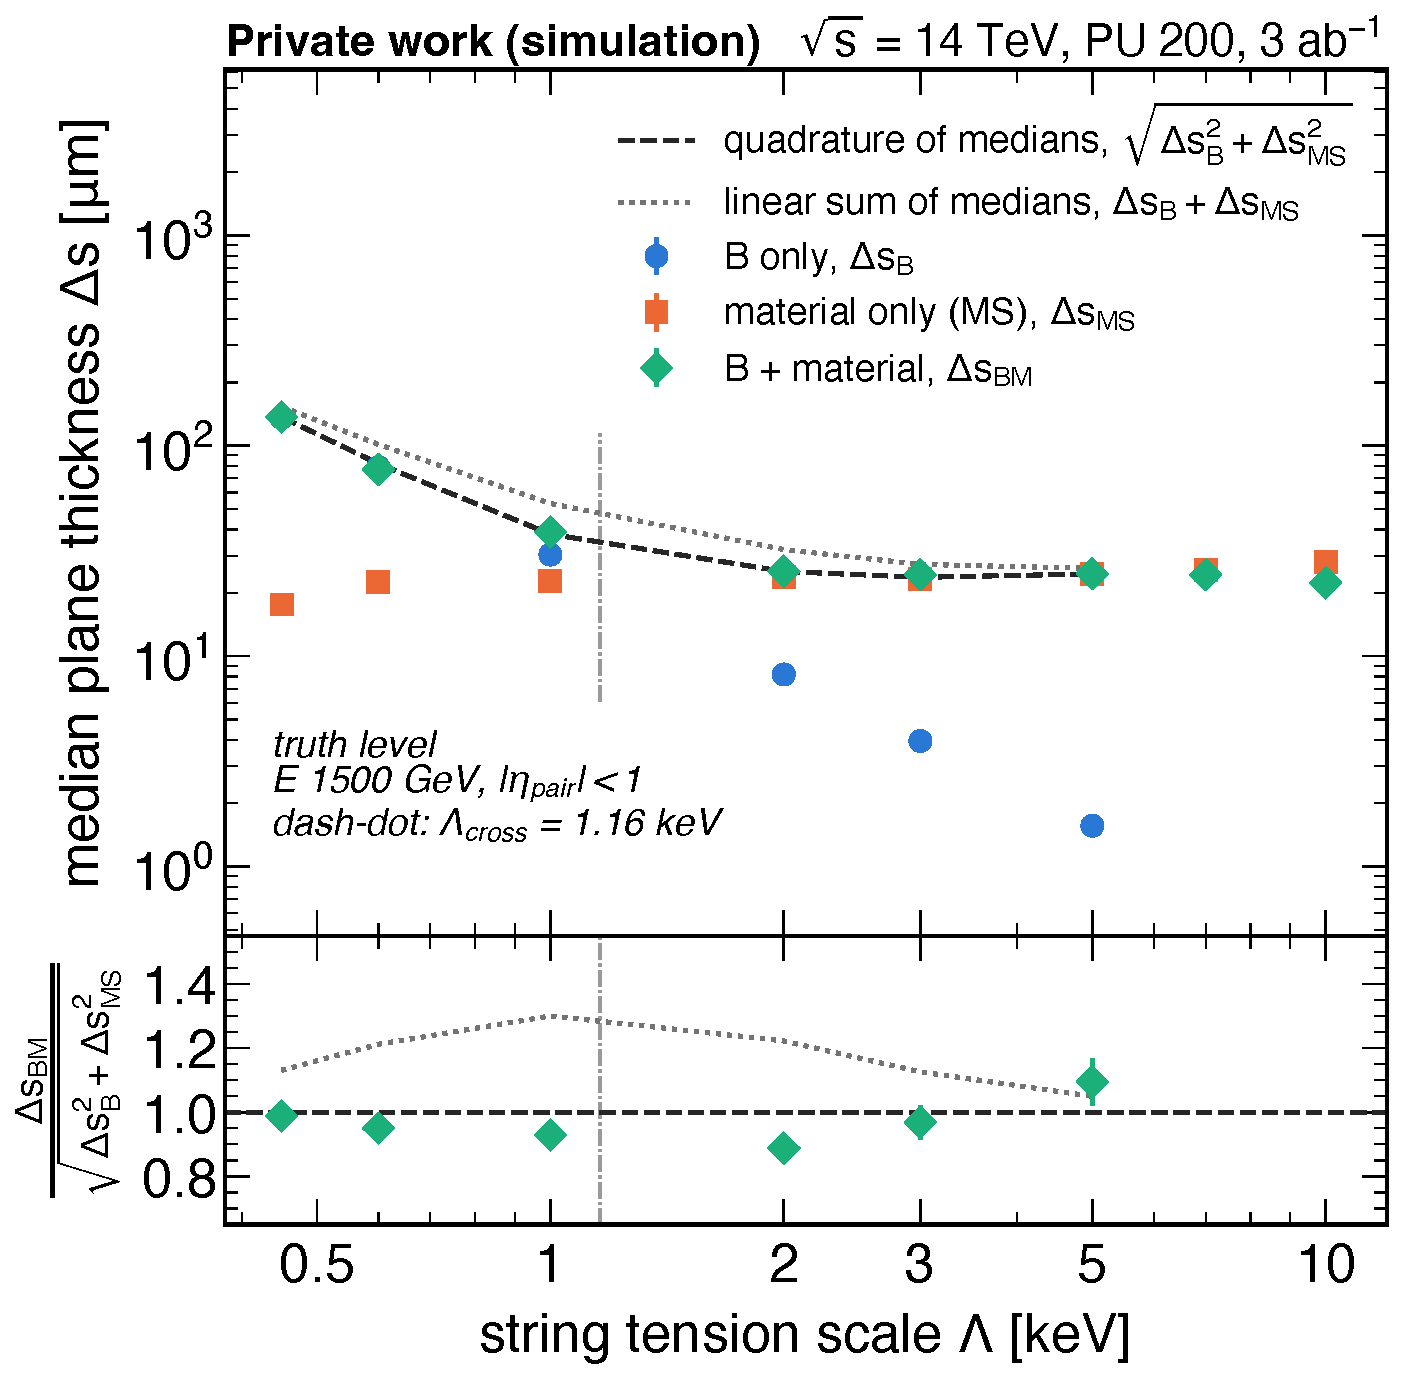
\includegraphics[height=0.34\linewidth]{figures/T1_u2_thickness_F_m1500.pdf}
\caption{B-field and multiple-scattering plane thickness at truth level for the fermion at $\mQ=200$ (top left), 500
(top right), 1000 (bottom left) and $1500\GeV$ (bottom right), $|\eta_{\rm pair}|<1$. Upper panels: median $\DsB$
(field only), $\DsMS$ (material only) and $\DsBM$ (both) against $\Lam$, with the quadrature and linear sums of the
medians; the dash-dot line marks $\Lcross$. Lower panels: $\DsBM$ over the quadrature sum. The field dominates below
$\Lcross\approx1.2$--$1.9\keV$ and the floor above; in the crossover region the two add below quadrature. Pile-up is
not simulated at truth level; the right-hand label gives the HL-LHC conditions of the study. The scalar ($\Etil$ at
$500\GeV$) behaves the same way (\rep{paper/figures/T1_u2_thickness_S_m500.pdf}).}
\label{fig:u2}
\end{figure}

\begin{figure}[htbp]
\centering
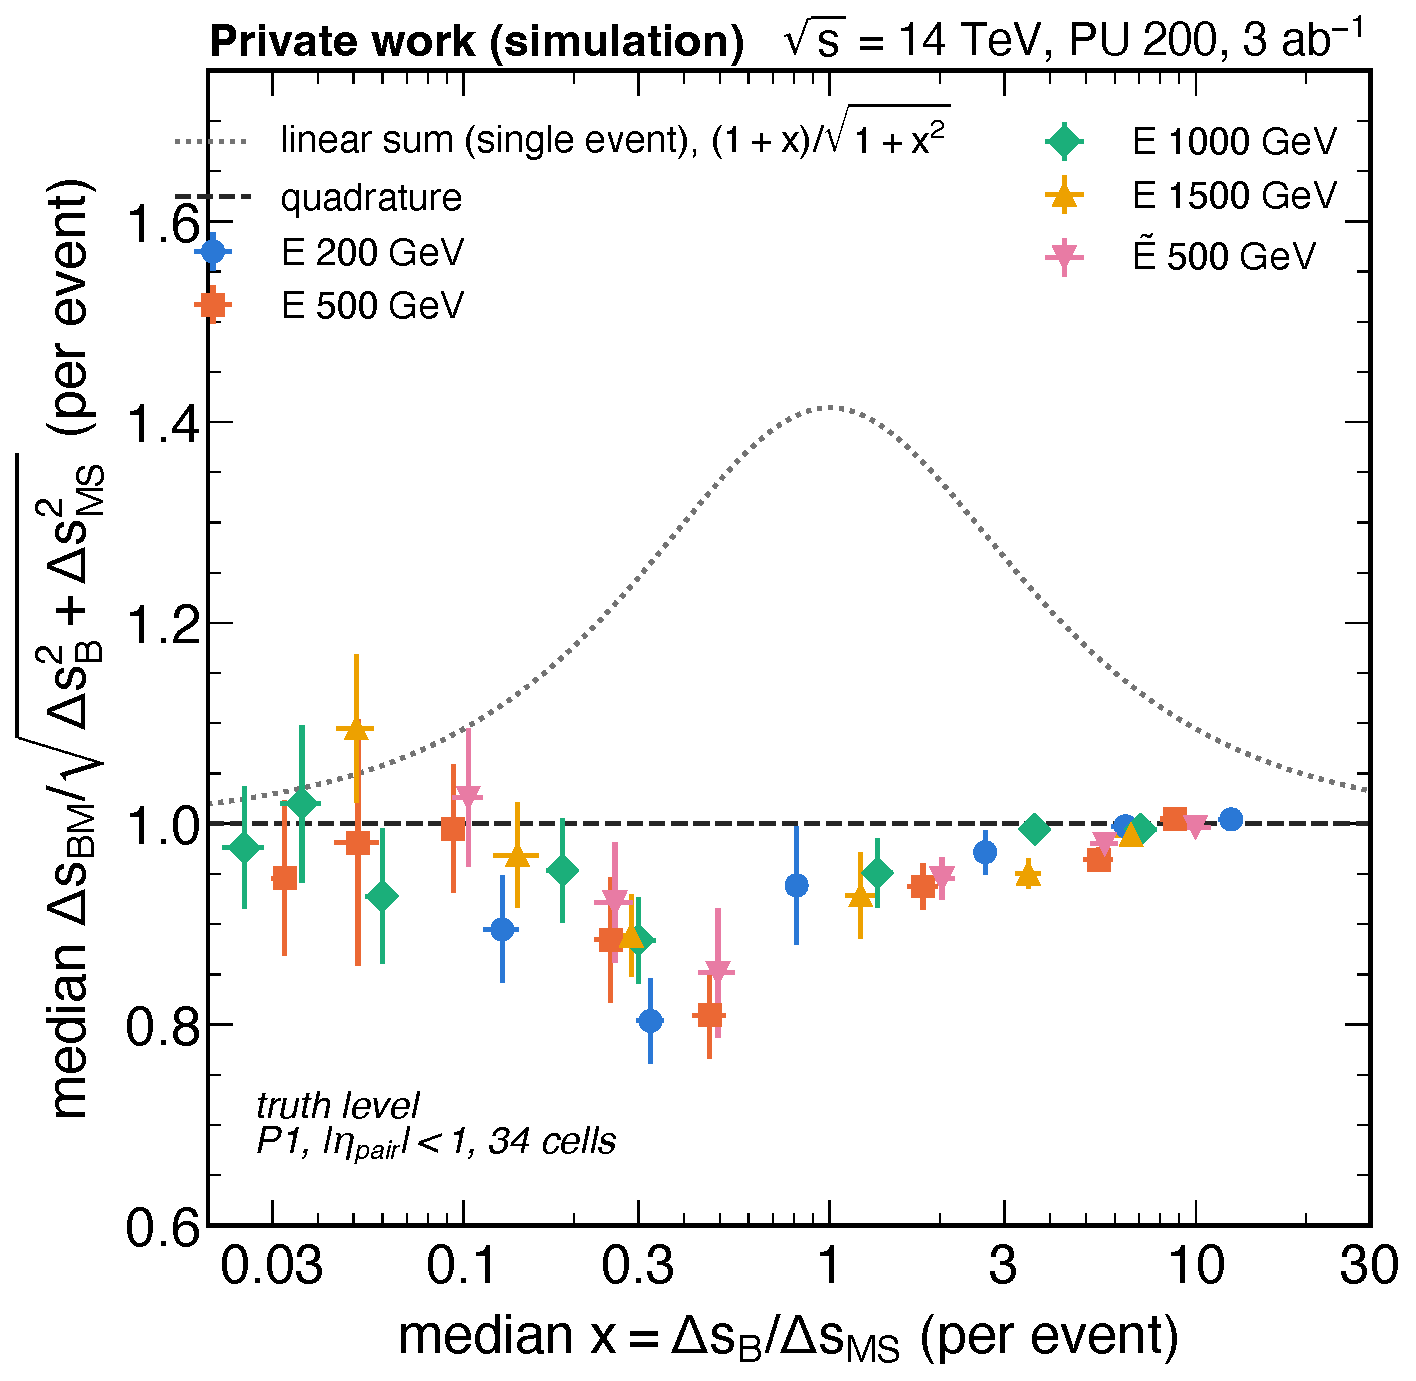
\includegraphics[height=0.37\linewidth]{figures/T2_u2_ratio_vs_x.pdf}\hspace{0.02\linewidth}
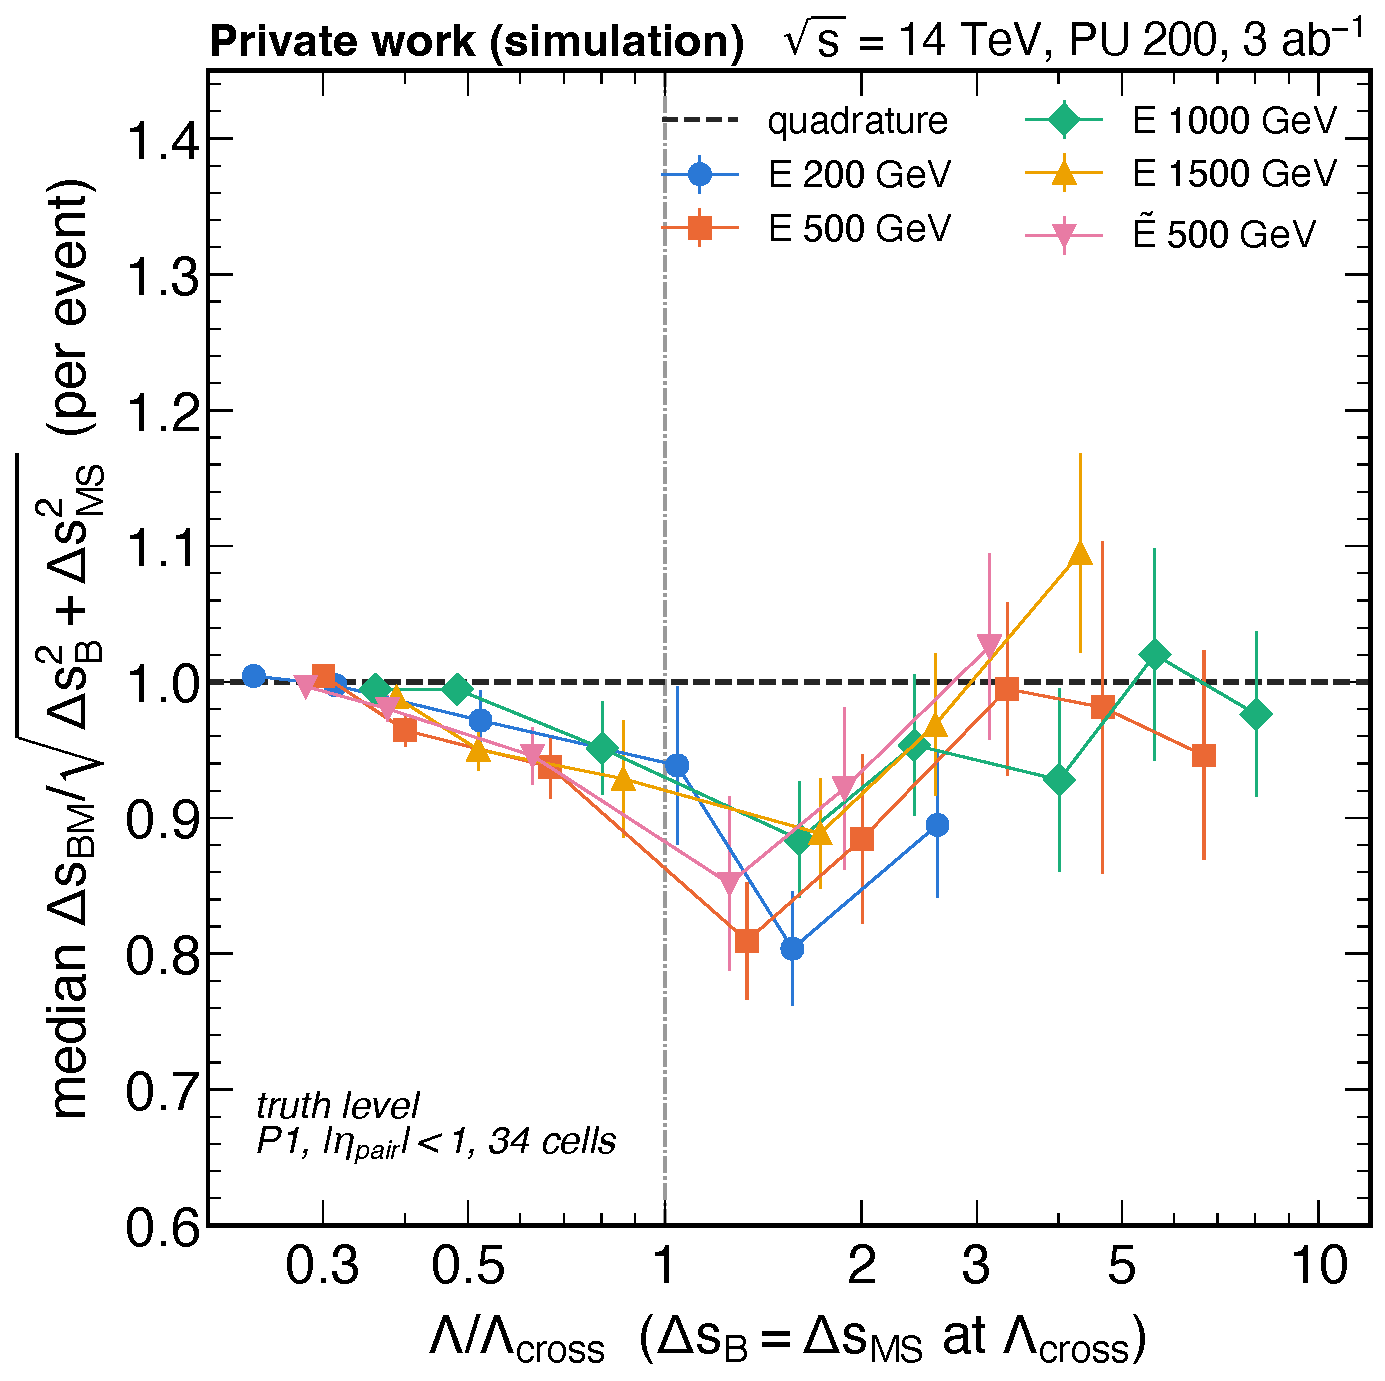
\includegraphics[height=0.37\linewidth]{figures/T3_u2_ratio_vs_lamcross.pdf}
\caption{Combination of the B-field and multiple-scattering thickness at truth level, all 34 cells of the P1 grid with
both measurements. (Left) Measured median $\DsBM/\sqrt{\DsB^2+\DsMS^2}$ against $x=\DsB/\DsMS$, with the curve for
a single event in which the two displacements add linearly. (Right) The same ratio against $\Lam/\Lcross$: the
sub-quadrature dip is deepest at $\Lam/\Lcross\approx1.25$--1.73. Pile-up is not simulated at truth level.}
\label{fig:u2ratio}
\end{figure}

\subsection{P1 in summary}\label{sec:p1:summary}
At truth level the B-field plane thickness of quirk pairs in the CMS solenoid is described by
$\DsB\propto\epsB[\ln(1/\epsB)+C]$, with a local slope $c\simeq0.10$--0.11 at $1\keV$ that falls with $\Lam$ as
predicted. The law is derived and confirmed by blind numerics at $1\keV$; on the full simulation it holds per event in
the window $\lmax/\RIT\lesssim0.6$, $\kB\lesssim4$, while the population median lies $+2$--$3\%$ above the prediction
at $1\keV$ (a failed $1.5\%$ gate, read as an estimator effect, \EST{}), and a larger $\kB$-dependent excess at
$3$--$5\keV$ is measured whose attribution to $\Bstar$ is estimated, not established. For $\Lam\gtrsim1.2$--$1.9\keV$
the thickness is set by multiple scattering at 10--28$\um$. Whether the B-field thickness survives at detector level was
not measured (user decision, Appendix~\ref{app:limits}): the detector-level study of Sections~\ref{sec:detector}--\ref{sec:mlam} uses the plane
thickness only through the finder tolerances.

\section{Detector model and simulation chain (P2)}\label{sec:detector}

The P2 study asks what survives of the truth-level quirk patterns in a realistic tracker at pile-up 200. This section
describes the detector model, the pile-up overlay, the digitisation and the standard tracking that removes helical tracks.
Everything is built from public information: the CMS Phase-2 Tracker~\cite{CMS:2017lum}, MIP Timing
Detector~\cite{Butler:2019rpu} and Level-1 Trigger~\cite{Zabi:2020gjd} Technical Design Reports of the CMS
detector~\cite{CMS:2008xjf} and the public tkLayout
geometry. The design is in \rep{acts/stage4/plan.md} (reviewed in nine rounds), the frozen definitions in
\rep{acts/stage4/WP_RULE.md}, and the validation in the G1, G1b and G3 reports under \rep{acts/stage4/}.

\subsection{Chain overview}\label{sec:detector:chain}
The Stage-3 truth hits (configuration with field and nominal material, smeared luminous-region vertex, all surfaces,
$|\eta_{\rm pair}|<4$ propagated) are injected, one ACTS event per physics event, into a pile-up event simulated on the
same surfaces with ACTS~\cite{Ai:2021ghi} (pyacts 48.0.0) and its fast simulation Fatras. Quirk and pile-up hits are then
digitised together, a standard combinatorial Kalman filter (CKF) finds helical tracks, and a dedicated finder searches
the remaining hits for planes through the primary vertex (Section~\ref{sec:strategy}). Pile-up events are not stored:
each is regenerated bit for bit from the job seed and the event index.

\subsection{Geometry and material}\label{sec:detector:geo}
Each of the 83 physical Stage-3 surfaces except the endcap timing layer (ETL) becomes a sensitive ACTS surface at its nominal position in the D111 layout:
cylinders for the barrel (four IT pixel layers TBPX, three PS layers TBPS, three 2S layers TB2S, the barrel timing layer
BTL) and discs for the endcaps. The Stage-3 material per layer (Section~\ref{sec:p1:prop}) is attached as surface
material; stacked layers split it over their two sensors. Every cylinder and disc is divided into 32 azimuthal sectors of
the same geometric surface, which leaves the hit positions unchanged and brings the CKF from 23--60\,s to 1.6--3.4\,s per event. The
ETL could not be included in the ACTS geometry (a volume-stacking limitation); no finder variable uses it. A muon gun gives the full
17-hit central pattern with every hit on its surface to $<0.1\um$, and the Fatras scattering angle behind the first pixel
layer agrees with the Highland formula~\cite{Highland:1975pq} (ratio 0.93 with the PDG definition). Two Fatras pitfalls
were found and fixed: the default minimum momentum of $0.5\GeV$ drops every low-momentum looper (set to $30\MeV$), and
the JSON material density must be given in ACTS-native units.

\subsection{Pile-up overlay and density normalisation}\label{sec:detector:pu}
Minimum-bias interactions are generated with Pythia~8.312~\cite{Bierlich:2022pfr} (CP5~\cite{CMS:2019csb},
$\sqrt s=14\TeV$, $\sigma_{\rm inel}=78.9$\,mb), with a Poisson number of mean 200 per event and vertices drawn from the
luminous region ($\sigma_z=45\mm$, $\sigma_t=190\ps$~\cite{Butler:2019rpu}; $\sigma_{xy}=5\um$, \EST{}).
$K^0_S$, $\Lambda^0$ and other hyperons are decayed by Pythia; charged particles and photons with $p_T>50\MeV$ and $|\eta|<4$
are passed to Fatras with multiple scattering, ionisation, bremsstrahlung and photon conversions. Fatras has no hadronic
interactions and does no decays in flight, and out-of-time pile-up is not simulated.

The resulting in-time density, $1.33\times10^5$ hits per event, is \emph{below} the Tracker TDR occupancies (which
include out-of-time pile-up and secondaries~\cite[Sec.~6.2.1, Fig.~6.3]{CMS:2017lum}) by a factor 2.3--3.7 in the IT
(the IT cluster size is not given in the TDR, \EST{}), 2.5--4.3 in the PS and 4.0--7.3 in the 2S layers, rising with
radius. Since a fake-rate estimate at too low a density would be optimistic, every pile-up event is \textbf{topped up}
per layer to the TDR occupancy (user decision, Appendix~\ref{app:limits}): $({\rm ratio}-1)$ times the event's own Fatras crossings are added
on each layer, with $z$ resampled from the layer's hits and uniform $\phi$; on stacked layers they are added as in/out
pairs, the conservative choice for the per-crossing counts. Each added crossing counts as its own interaction in the
pile-up extrapolation (Section~\ref{sec:bkg:pu}). The lower and upper ends of the ratio ranges are a systematic.

\subsection{Digitisation, merging, timing and efficiency}\label{sec:detector:digi}
Hits are digitised by Gaussian smearing with binary resolutions (pitch$/\sqrt{12}$, as the TDR confirms for the
OT~\cite[Sec.~12.2]{CMS:2017lum}), with ACTS cluster merging switched off; two measurements on the same sensor are merged
at analysis level when they lie within one pitch in both local directions (user decision, Appendix~\ref{app:limits}), with the mean
position, an error of $\max(\sigma,|\Delta|/\sqrt{12})$ and summed energy. This sets the hit-level merging of the two
quirks at high $\Lam$. Table~\ref{tab:digi} lists the resolutions. Quirk hits arriving later than $\Delta t_{\rm
acc}=25\ns$ after a prompt particle would (one bunch crossing, following Ref.~\cite[Sec.~IV]{Knapen:2017kly}; variation
$12.5\ns$) are dropped, and a flat 99\% hit efficiency is applied (\UNV{}; variation 97\%).

\begin{table}[htbp]
\centering
\caption{Digitisation model (binary resolution, pitch$/\sqrt{12}$; \rep{plan.md} \S1.5). Pitches from the Tracker
TDR~\cite{CMS:2017lum} and the public D111 module table; BTL from the MTD TDR~\cite{Butler:2019rpu}.}
\label{tab:digi}
\small
\begin{tabularx}{\linewidth}{lccc>{\raggedright\arraybackslash}X}
\toprule
module & pitch & $\sigma_{r\phi}$ & $\sigma_{\rm long}$ & variation\\
\midrule
IT pixel & $25\times100\,\mu$m$^2$ & $7.2\um$ & $28.9\um$ & charge-sharing 3--6 / 11--24$\um$\\
PS (strip/macro-pixel) & $100\um\times1.467\mm$ & $28.9\um$ & $423\um$ & $\pm20\%$\\
2S (strips) & $90\um\times50.27\mm$ & $26.0\um$ & $14.5\mm$ & uniform smearer\\
BTL (timing) & bars $57\mm\times3.12\mm$ & $16\mm$ (\EST{}) & $0.9\mm$ & $\sigma_t=35\ps$; 60\,ps end of life\\
\bottomrule
\end{tabularx}
\end{table}

\subsection{Standard tracking and hit removal}\label{sec:detector:ckf}
Quirk tracks are not helices, so the CKF is used only to remove the hits of helical tracks before the quirk finder runs:
seeds from triplets of IT space points with $p_T>0.9\GeV$, $|z_0|<200\mm$, tracks with $\ge7$ measurements, $\le2$ holes
and $|d_0|<4\mm$, following the ``unassociated hits'' logic of Ref.~\cite[Sec.~III.D]{Knapen:2017kly}. In the production chain 13.9\% of all
measurements (19.5\% of the barrel hits, $\approx1540$ tracks per event) are removed; low-$p_T$ pile-up hits stay and form the combinatorial background. The fraction $f_{\rm CKF}$
of a candidate's band hits that sit on CKF tracks is a selection variable (Section~\ref{sec:strategy:finder}); on the probe
samples no quirk measurement was taken by a CKF track (0 of 208).

\subsection{Primary vertex, MET and trigger model}\label{sec:detector:pvmet}
The primary vertex is the true hard-scatter vertex smeared by $(\sigma_{xy},\sigma_z)=(10,15)\um$ with a 93\%
identification efficiency at pile-up 200 (graphical readings of the Tracker TDR~\cite{CMS:2017lum}, \UNV{}). The missing
transverse momentum is the truth $p_T(Q\bar Q)$ (the quirks deposit $\lesssim5\GeV$ in the calorimeters, carried as a
one-sided $\lesssim2\%$ bias) smeared by $\sigma_\perp=25\GeV$ per component (15 and $35\GeV$ variations; the PUPPI MET
resolution at pile-up 200 is \UNV{}). The trigger and preselection model is part of the selection and is given in
Section~\ref{sec:strategy:trig}.

\subsection{Samples}\label{sec:detector:samples}
Table~\ref{tab:samples} lists the detector-level samples. Production ran on one laptop (Apple M3, 8 cores) in three
campaigns of about one day each (C1a, C1b, C2B) plus a full-chain re-run of nine signal points (A2FC): 2295 jobs, no job
errors, $\approx382$ CPU-hours. About 0.14\% of pile-up events hit an ACTS navigation assertion at the $\phi$-sector
boundaries; they are replaced deterministically by a re-seeded event and recorded (three G3 pilot jobs that failed this way
before the fix were left out).

\begin{table}[htbp]
\centering
\small
\caption{Detector-level samples (\rep{acts/stage4/C1_LAUNCH.md}, \rep{G1B_REPORT.md}, \rep{A2FC_REPORT.md}).
$\rho$ is the pile-up density in units of a normalised PU-200 event (Section~\ref{sec:bkg:pu}).}
\label{tab:samples}
\begin{tabularx}{\linewidth}{lX}
\toprule
sample & content and purpose\\
\midrule
A1 & signal without pile-up: finder-efficiency calibration and the window/tolerance variations\\
A2 & signal + PU 200 on five (species, mass) points ($E$ 200, 500, 1000, 1500; $\Etil$ 500) $\times$ 8 $\Lam$ values, run row-major
     (the same pile-up event for every $\Lam$ of a row), $\Lam=0.45,0.6,0.85,1,1.5,2,3,5\keV$, 180--200 template events
     per point\\
A5 & five (species, mass) points at $\Lam=1\keV$ through the full ACTS chain with dumps (closure of the fast signal path)\\
A2FC & full-chain re-run of the nine A2 points where the fast signal path was not validated (pre-registered revert rule)\\
B1 & pile-up only, $\rho=1$, four MET roads per event: 12\,000 events, 48\,000 trials\\
B2 & pile-up only, $\rho=2$ (superposition of two normalised events): 3000 events, 6000 trials\\
dens & $\rho=1$ re-runs of a B1 subset with the top-up at its lower and upper ratio (density systematic)\\
SM & Pythia~8 $Z(\nu\nu)$+jet, $W(\ell\nu)$+jet (incl.\ $\tau$ split by decay class), $t\bar t$, with PU 200 and truth MET$>200\GeV$;
     2000 events per sample\\
C$'_0$, C$'_{\rm PU}$ & guns and toys for single-interaction topologies (photon conversions, $V^0$, vertex pairs, loopers,
     nuclear interactions, decays in flight): $3\times10^4$--$10^5$ per gun or toy without pile-up, 500 per topology (8 topologies) with
     pile-up\\
\bottomrule
\end{tabularx}
\end{table}

\section{Analysis strategy and the pre-registered working-point rule (P2)}\label{sec:strategy}

The finder must select quirk planes at a pile-up fake rate of order $10^{-9}$ per triggered event, far below what can be
measured directly. The strategy therefore separates three steps that are fixed in this order: (i) a finder and an ordered
ladder of selections defined on background samples only; (ii) a rule, frozen before any signal efficiency was computed,
that picks the working point (WP) from the background estimates; (iii) a pre-defined fallback deliverable if no rung
satisfies the rule. This section defines all three; the frozen text is \rep{acts/stage4/WP_RULE.md} (sha256
\texttt{1b2ea9bd\ldots}) with the amendment \rep{WP_RULE_PC19.md}, and every later change is logged in
\rep{acts/stage4/HASH_ADDENDUM.md}.

\subsection{Trigger and offline preselection}\label{sec:strategy:trig}
The quirks are nearly invisible to the calorimeters, so the event is triggered by the missing transverse momentum (MET)
from initial-state radiation, as in previous proposals~\cite{Knapen:2017kly,Li:2019wce}; the Level-1 track trigger is
not used, because quirk hits form few stubs and no helices. The trigger is modelled as an efficiency on the smeared
MET: $\Eff_{\rm trig}=0.98\cdot\frac12\{1+\operatorname{erf}[(\mathrm{MET}-200\GeV)/(\sqrt2\cdot20\GeV)]\}$ (\EST{};
the Phase-2 L1 PUPPI-MET thresholds~\cite{Zabi:2020gjd} are carried as $\pm25\GeV$ on the turn-on point). The offline
preselection requires MET$\,>250\GeV$, at least one jet with $p_T>100\GeV$ and $|\eta|<2.4$, $\min\Delta\phi(\text{jet}_{1-4},
\text{MET})>0.5$, and vetoes isolated electrons and muons ($p_T>10\GeV$), hadronic $\tau$ ($p_T>20\GeV$) and photons
($p_T>15\GeV$); the vetoes cost the signal nothing and act only on the SM backgrounds. The Stage-3 signal samples
contain only pairs with $p_T(Q\bar Q)>200\GeV$ (and $|\eta_{\rm pair}|<4$), the recoil tail that the trigger selects, so
the yield carries the tail fraction $f_{200}$ of the inclusive cross section (Table~\ref{tab:xsec} for $E$: 0.048, 0.104, 0.146
and 0.169 at 200, 500, 1000 and $1500\GeV$; 0.114 for $\Etil$ at $500\GeV$). The signal efficiency factorises into
$f_{200}$, a truth-level acceptance $A$ of the tail sample and a detector-level selection efficiency $\Eff_{\rm sel}$:
\begin{equation}
  N_{\rm exp}=\sigma_{\rm norm}\,f_{200}\,L\,A,\quad A=\Eff_{\rm fid}\,\Eff_{\rm trig}\,\Eff_{\rm presel|trig}\,\Eff_{\rm PV},
  \quad S=N_{\rm exp}\,\Eff_{\rm sel},\quad \Eff_{\rm tot}=f_{200}\,A\,\Eff_{\rm sel},
  \label{eq:effchain}
\end{equation}
with $L=3\abinv$ and the inclusive $\sigma_{\rm norm}$ of Eq.~\eqref{eq:signorm}. $\Eff_{\rm fid}$ is the fraction of tail
pairs with $|\eta_{\rm pair}|<2.5$, $\Eff_{\rm presel|trig}$ the preselection efficiency after the trigger and
$\Eff_{\rm PV}=1$ (PV identification not modelled); $A_{\rm incl}=f_{200}A$ is the acceptance relative to the inclusive
cross section (Table~\ref{tab:acc}). $N_{\rm exp}$ is the predicted signal yield in the acceptance, $\Eff_{\rm sel}$ the
fraction of these events with a signal-matched candidate that passes the selection at pile-up 200 and has
$f_{\rm CKF}<0.2$ (events whose quirks did not both leave the tracker in the truth simulation count as failures), and $S$
the expected number of selected signal events; the factorisation assumes $\Eff_{\rm sel}$ independent of the
preselection. From Section~\ref{sec:results} on, $\Eff$ without subscript means $\Eff_{\rm sel}$. A candidate counts as signal-matched only if at least three of its core hits on at least three layers
are quirk hits and quirk hits are at least half of its core hits (declared before any signal efficiency was looked at).

\subsection{The plane finder}\label{sec:strategy:finder}
The baseline finder (F0) looks for a plane through the primary vertex (PV) that contains repeated crossings of the same
layers, in the azimuthal road of the MET. In PV coordinates $\mathbf u=\mathbf x-\mathbf x_{\rm PV}$:
\begin{enumerate}
\item \textbf{Road and window.} Hits must satisfy $|\Delta\phi(\mathbf u,\phi_{\rm MET})|<\dninetyfive+\arcsin\min(1,W_c/r)$,
  lie forward of the PV along the plane axis and within $|\mathbf u\cdot\hat n_2|<W_c$ of it, with $W_c=75\mm$ (half the
  outer IT radius, rounded up, from $\lmax\le\RIT$). The road half-width $\dninetyfive=0.15$\,rad is the 95\% quantile
  of $|\Delta\phi(\mathrm{MET},p_T(Q\bar Q))|$ at generator level after trigger and preselection, maximised over the 17
  (species, mass) points (no detector response; 0.130--0.149\,rad per mass).
\item \textbf{Seeds.} Pairs of hits on the outer two IT barrel layers with $|\Delta\phi|<0.3$, $|\Delta\eta|<0.2$, confirmed
  by a third hit on the second layer, define a plane normal $\hat n$; a seed is refitted if at least $\Tseed$ layers have
  $\ge2$ crossings in its band. $\Tseed=6$ was frozen and changed to $\Tseed=4$ by the action pre-declared for the G3 pilot
  (Section~\ref{sec:bkg:closure}).
\item \textbf{Collection and refit.} Hits with $|\hat n\cdot\mathbf u|<3\sigma_{\rm tot}$, where
  $\sigma_{\rm tot}^2=\sigma_n^2+t_{\rm tol}^2$, $\sigma_n$ is the hit resolution projected on $\hat n$ and
  $t_{\rm tol}=30\um$ is the plane-thickness tolerance (the truth-level B+MS thickness is 10--30$\um$ above
  $\Lcross\approx1.2$--$1.9\keV$, Section~\ref{sec:p1:ms}). Three iterations of a PV-constrained weighted plane fit follow; duplicate
  candidates within 2\,mrad are merged.
\item \textbf{Variables.} Per-layer crossing counts (on stacked OT modules the minimum of the two sensors): $N_{\rm IT2}$, $N_{\rm
  IP2}$ and $N_{\rm 2S2}$ count IT, IT+PS and 2S barrel layers with at least two crossings. The robust core width
  $\wcore=1.4826\,\mathrm{MAD}(\mathbf u\cdot\hat n_2)$ over the in-band IT and PS hits measures the ribbon width (a proxy of
  $\lmax$), and $\chicore$ is the plane-fit $\chi^2$ of the core hits with its $p$-value. $f_{\rm CKF}$ is the fraction of
  band hits that sit on CKF tracks.
\item \textbf{Fixed cuts at every rung.} $N_{\rm IT2}\ge3$, $|\Delta\phi(\hat n_3,\mathrm{MET})|<\dninetyfive$,
  $|\eta(\hat n_3)|<1.0$ and $f_{\rm CKF}<0.2$ (the last not credited for the pile-up background). The pseudorapidity cut on
  the plane axis $\hat n_3$ restricts the analysis to the barrel (user decision, Appendix~\ref{app:limits}); 1.0 is the edge of the third 2S
  layer (0.94) rounded up, a geometry-only number.
\end{enumerate}
The improved variant (F1) adds three quirk-hypothesis variables computed from the stored hits: a helix test $h$ (with the
PV and with a free origin), the linearity $o$ of the opening of the two arms, and a truncated-mean $dE/dx$ in MIP units, the pooled truncated mean of all
muon-gun TBPX hits ($3.558\times10^{-4}\GeV$). Candidates are split into two categories: \textbf{SR-T},
in which the earliest in-band BTL hit is late by $\Delta t=t_{\rm BTL}-t_{\rm PV}-|\mathbf u|\in[t_{\min},t_{\max}]$
(natural units), where $t_{\min}$ is set where the per-hit rate of in-time pile-up falls to $10^{-4}$ and
$t_{\max}$ where that of the next bunch crossing rises to $10^{-4}$, both from pile-up-only events (logged amendment, Appendix~\ref{app:limits}; $\sigma_{t,\rm PV}=190\ps$, varied to 150 and 230\,ps), and \textbf{SR-G}, all others.
The binding window, from the production pile-up-only sample, is $[5.955,\,24.035]\ns$, and the
pre-registered time-independence test passes.

\subsection{The ladder}\label{sec:strategy:ladder}
Each category walks its own copy of a ladder of 23 cumulative rungs (Table~\ref{tab:ladder}); each rung tightens one
threshold of the previous one. The order is fixed by background considerations only: counting rungs first (the base of
the pile-up extrapolation), then width, core $\chi^2$, 2S layers and the F1 variables. There is no fixed cut on the plane
width; the width thresholds are rungs.

\begin{table}[htbp]
\centering
\small
\caption{The frozen ladder (\rep{WP_RULE.md} \S3), applied with the fixed cuts of Section~\ref{sec:strategy:finder}.
Each rung adds the stated requirement to all previous ones. R04 ($N_{\rm IP2}\ge7$) means a double crossing on every
IT and PS barrel layer.}
\label{tab:ladder}
\begin{tabular}{lll}
\toprule
rungs & family & requirement added\\
\midrule
R01--R04 & F0 counting & $N_{\rm IT2}\ge3$ and $N_{\rm IP2}\ge4,5,6,7$\\
R05--R08 & F0 width & $\wcore<37.5,\,18.75,\,9.4,\,4.7\mm$ ($W_c/2^k$, $k=1\ldots4$)\\
R09--R11 & F0 core $\chi^2$ & $p(\chicore)>10^{-3},\,0.01,\,0.05$\\
R12--R14 & F0 2S & $N_{\rm 2S2}\ge1,2,3$ (R14 = full F0)\\
R15--R17 & F1 helix & $h>2,3,5$\\
R18--R20 & F1 opening & $o>2,3,5$\\
R21--R23 & F1 $dE/dx$ & $dE/dx>1.3,\,1.6,\,2.0$ MIP\\
\bottomrule
\end{tabular}
\end{table}

\subsection{Background budget and the working-point rule}\label{sec:strategy:rule}
For each category $\kappa\in\{\text{T},\text{G}\}$ (SR-T, SR-G) and rung $r$ the expected background in $3\abinv$ is the sum
\begin{equation}
  \Nbkg = \Ntrig\Big[P_{\rm PU}+P_{\rm SM,HS}+\sum_t \text{rate}_t\,P(\text{pass}\mid t)\Big]+N_{\rm cosmic}+N_{\rm halo},
  \label{eq:bsum}
\end{equation}
where $\Ntrig$ is the number of SM events after trigger and preselection, $P_{\rm PU}$ the pile-up-only fake probability
per event, $P_{\rm SM,HS}$ that of candidates involving hard-scatter hits, and $t$ runs over single-interaction
topologies (conversions, $V^0$, PV pairs, loopers, nuclear interactions, decays in flight) with generator-level rates
(Section~\ref{sec:bkg}). Each term is a product of measured factors with a log-normal uncertainty,
$\sigma_{\ln}^2=\text{stat}^2+(\text{extrapolation model})^2+(\text{density})^2+(\text{normalisation})^2$, and
$\Nbkgeightyfour$ is the 84th percentile of the Monte-Carlo sum. A factor with zero observed counts enters once per term,
at $1.14/M$ (the one-sided 68\% Poisson bound for a population of size $M$) with $\sigma_{\ln}=1$, never as zero.

\paragraph{Rule.} The per-category WP is the loosest rung $r^*_\kappa$ with $\Nbkgeightyfour\le0.11$ events for it and every
tighter rung. The value 0.11 follows from log-normal algebra alone: two independent categories at $\sigma_{\ln}=2.3$
combine at 2.71 times the per-category $\Nbkgeightyfour$, and $0.3/2.71=0.11$. If both categories have a WP, the pair is
accepted only if the combined $\Nbkgeightyfour\le0.3$ for it and for every tighter pair, with a deterministic continuation
otherwise. If no rung qualifies, the category has no WP: the user is told, and the pre-defined fallback applies. No
re-ordering of the ladder and no new rung are allowed after the freeze, and further production is decided on cost and
background reach, never on signal yields.

\subsection{The fallback deliverable}\label{sec:strategy:fallback}
The fallback (WP\_RULE \S8, approved by the user before production) defines one admissible selection per
hypothesis from truth-level quantities published in Stage~3, so that a selection never cuts away the hypothesis it tests:
\begin{itemize}
\item a width rung is admissible only if $\Lam\ge\Lam_R(\mQ)\,2^{(k+1)/2}$, where $\Lam_R(\mQ)$ is the smoothed $\Lam$
  at which the median $\lmax$ equals $\RIT$ (Fig.~\ref{fig:edges}); $k_{\rm adm}\in\{0,\ldots,4\}$ is the largest such $k$;
\item a $dE/dx$ rung is admissible only if its threshold is below $R_{\rm eff}/1.25$, where $R_{\rm eff}$ is the expected
  truncated-mean ionisation of the quirk at its IT velocity, diluted by pile-up hits in the core (a frozen mixture model
  using the PDG restricted-loss formula for silicon~\cite{ParticleDataGroup:2024cfk}); this happens only at the tightest
  width rung for heavy masses;
\item the fallback selection is $r_{\rm fb}={\rm FB}_{k_{\rm adm}}\wedge h>5\wedge o>5\,(\wedge\,dE/dx>e_{\rm adm})$, plus
  the time tag in SR-T, where ${\rm FB}_k\equiv N_{\rm IT2}\ge3\wedge N_{\rm IP2}\ge7\wedge p(\chicore)>0.05\wedge
  N_{\rm 2S2}\ge3\wedge\wcore<W_c/2^k$ is the non-width part of R14 with a single width cut (FB0: no width cut);
  $e_{\rm adm}$ is the largest admissible $dE/dx$ threshold.
\end{itemize}
The primary result at each $(\mQ,\Lam,\kappa)$ is the admissible WP if it exists, otherwise the fallback selection with its
non-zero log-normal background. Choosing the best selection per point is forbidden. Efficiencies and backgrounds are also
reported at five fixed reporting selections R$_A$ (end of counting) to R$_E$ (full F1), without limits.

\paragraph{Statistical treatment.} The signal strength is the yield $\mu$ in the acceptance, with
$\mu\,\Eff_{{\rm sel},\kappa}$ expected selected events in category $\kappa$ ($\mu=N_{\rm exp}$ for the prediction).
Its expected 95\% CL upper limit $\mu_{95}$ per $(\mQ,\Lam)$ uses a two-bin
(SR-T, SR-G) counting likelihood with each background as a log-normal nuisance and the CL$_s$
method~\cite{Junk:1999kv,Read:2002hq}, evaluated with hybrid toys (5000 per point; primary) and the asymptotic
formulae~\cite{Cowan:2010js} as a cross-check, in an in-house implementation. After the last analysis fix (a
saturated-likelihood offset in the asymptotic mode) the asymptotic/toy ratio of the limits is 0.32--1.07 on the final
run: 1.02--1.07 where one category carries all the signal, 0.32--0.72 where both do and $\sigma_{\ln}$ is large, a
genuine difference between the two methods. Toys are therefore primary, and the asymptotic $\pm1\sigma$ bands are not
used. A comparison with pyhf~\cite{Heinrich:2021gyp} exists only for the dry run before that fix and is not claimed for the final
code. The limit on the inclusive cross section is $\sigma_{95}=\mu_{95}/(L\,f_{200}\,A)$, so that
$\sigma_{95}/\sigma_{\rm norm}=\mu_{95}/N_{\rm exp}$ (the figures label $\sigma_{\rm norm}$ as $\sigma_{\rm th}$); a ratio
below one would be an exclusion. Because $\mu_{95}$ is a limit on the yield, the signal-normalisation uncertainties
(the $\pm5\%$ on $\sigma_{\rm norm}$ and the tail rate of Section~\ref{sec:model:syst}) do not enter it.

\subsection{Blinding, freeze and logged changes}\label{sec:strategy:freeze}
The rule, the finder code and its configuration were hash-frozen before the first signal efficiency (the only
signal-derived inputs are generator- or truth-level quantities that the plan pre-declares: $\dninetyfive$, the IT
velocities and $\Lam_R$). Every later change is logged in \rep{acts/stage4/HASH_ADDENDUM.md} and was pre-declared or
regression-tested: runner hooks and a recovery for an ACTS navigation assertion (bit-identical on the existing job kinds);
analysis-level fixes from the analysis reviews, which changed background estimates but no selection; $\Tseed=6\to4$
(G3 pilot, Section~\ref{sec:bkg:closure}); the SR-T window, because the frozen window $[t_{\min},25\ns]$ was empty once
next-crossing hits were included; and the full-chain re-run (A2FC) of nine signal points under the pre-registered revert
rule.

\section{Backgrounds (P2)}\label{sec:bkg}

Any two straight lines through the primary vertex are coplanar with it, and at pile-up 200 the inner tracker contains
$\sim10^5$ hits per event, so coplanar patterns arise both from random combinations of pile-up hits and from SM
topologies with a vertex on a line through the PV. This section describes how each background term of
Eq.~\eqref{eq:bsum} is estimated. The methods are pre-registered (\rep{plan.md} \S4, \rep{WP_RULE.md} \S4, \S6, \S7);
the numbers are from the final analysis run (C12FC\_v1, \rep{acts/stage4/STAGE4_RESULTS.md} \S1--3).

\subsection{Pile-up-only fake rate}\label{sec:bkg:pu}
A WP needs a pile-up fake probability of order $10^{-9}$ per triggered event, while a direct measurement would need
$\gtrsim10^9$ simulated pile-up events. The probability is therefore measured directly where possible and extrapolated
otherwise, by two pre-registered methods.
\begin{itemize}
\item \textbf{Direct ladder} (sample B1): pile-up-only events at the normalised density ($\rho=1$), each searched in four MET
  roads $\pi/2$ apart with a PV drawn from the luminous region independently of the pile-up vertices. The per-trial rate
  (mean over roads) is the primary estimator, because a data event has exactly one MET road.
\item \textbf{Interaction-count thinning} (sample B2): pile-up at $\rho=1$ is exactly a Poisson thinning, keeping each
  interaction with probability $q=1/\rho$, of the superposition of $\rho$ independent normalised events. For a candidate
  found at density $\rho$ whose in-band hits come from the interaction set $S$, the expected number of passing candidates
  at $\rho=1$ is weighted by
  \begin{equation}
    w_r=\sum_{T\subseteq S\ \text{passes}\ r} q^{|T|}(1-q)^{|S|-|T|},
    \label{eq:thinning}
  \end{equation}
  computed exactly by a per-layer dynamic programme for the counting rungs and by conditional importance sampling for
  the per-subset rungs. A candidate needing $n_{\rm int}$ specific interactions enters with $\rho^{-n_{\rm int}}$, so the
  method reaches deep into the tail without a fitted exponent; each top-up crossing counts as its own interaction.
  Candidates are counted once per distinct passing hit set (sets sharing $\ge50\%$ of their hits are one).
  Check of Eq.~\eqref{eq:thinning}: for $q=1$ it returns the pass indicator of the full set (verified on 2000 sets).
\item \textbf{Rung factorisation} beyond the reach of both: conditional pass fractions measured on the tightest population
  with at least ten entries, with a pre-registered factorisation (independence) test whose correlation factor
  multiplies the estimate if it exceeds one at $2\sigma$.
\end{itemize}

\subsection{Closure of the extrapolation and the seed threshold}\label{sec:bkg:closure}
The thinning prediction from $\rho=2$ is tested against the direct $\rho=1$ count at the deepest rung where both have
statistics (test T1 at R04, T1w at the first width rung), with the pre-registered criterion $|z|<2$. In the G3 pilot
(127 of 130 pile-up-only jobs) the test \textbf{failed in the anti-conservative direction} ($N_{\rm obs}/N_{\rm pred}=1.32$,
$z=+14.3$, for T1; 1.42, $z=+17.6$, for T1w; over-merging of hit sets at $\rho=2$). By user decision the pre-registered
conservative end state applies: the pile-up estimate is multiplied by the observed factors (compounded at deeper rungs),
the trend enters $\sigma_{\ln}$, and the closure is re-measured in production. The pilot also triggered the pre-declared
action $\Tseed:=4$ (pass fraction moved by more than $2\sigma$ between $\Tseed=6$ and 4).
On the production samples at $\Tseed=4$ (B1: 48\,000 trials; B2: 6000 trials) the closure is again
anti-conservative: $N_{\rm obs}/N_{\rm pred}=1.500$ ($z=+52.8$) for T1 at R04 and 1.606 ($z=+59.4$) for T1w at R05 (the
lever-arm requirement fails at R06). The compounded factor $\times2.41$ multiplies the pile-up estimate at every rung
from R05 on, and the significant downward trend of the ratio along R04--R07 ($-0.36$ per rung) enters only
$\sigma_{\ln}$, linearly in the rung index. The $dE/dx$ closure test is untestable (fewer than ten counts) and the
factorisation test is degenerate, so \textbf{beyond R06 (the deepest rung with ten counts at $\rho=2$; R07 for the direct
B1 count) the pile-up estimate rests on rung factorisation without an informative cross-variable closure test}. The
thinning reach is $\approx1.7\times10^{-10}$ per trial (\EST{}), against $\approx2.7\times10^{-10}$ that the pile-up term
alone would need to fill the whole SR-G budget: the reach would suffice in principle, but the deepest rung with at least
ten $\rho=2$ counts is R06. The $\sigma_{\ln}$ of the pile-up term is dominated by the density
normalisation (1.15--1.89) at loose rungs and, from R11 on, by the trend term (2.0 to 6.3) and the spread between
extrapolation models (4.76); the F1 helix and opening variables pass every pile-up record and earn no credit.

\subsection{SM hard-scatter backgrounds and normalisation}\label{sec:bkg:sm}
Two prompt tracks from the PV are coplanar with it; $W\to\tau\nu$ with a three-prong $\tau$, a lost lepton with a track,
or the underlying event can therefore fake a plane if the tracks escape the CKF removal. These are estimated from
Pythia~8 samples of $Z(\nu\nu)$+jet, $W(\tau\nu)$+jet (split by $\tau$ decay class) and $t\bar t$ (one lepton) with
pile-up 200 and truth MET$\,>200\GeV$, normalised to $\Ntrig$, the number of SM events after the trigger and the offline
preselection (user decision, Appendix~\ref{app:limits}). Candidates with at least one hard-scatter hit are assigned to $P_{\rm SM,HS}$; pure
pile-up candidates belong to $P_{\rm PU}$. These samples exist only at $\rho=1$, so their depth comes from rung
factorisation alone. Processes not simulated at detector level ($W(e\nu)$, $W(\mu\nu)$, $t\bar t$ dileptonic, single top, dibosons) enter
$\Ntrig$ with conservative proxies.
After trigger and preselection $\Ntrig=4.08\times10^7$ ($\pm2.0\%$ statistical; generator-level Pythia, \EST{} as
physics): $Z(\nu\nu)$+jet $2.5\times10^7$, $W(\tau\nu)$ $7.7\times10^6$ (hadronic and leptonic $\tau$), $W(e\nu)$ and
$W(\mu\nu)$ $4.8\times10^6$, $t\bar t$ (one lepton) $2.4\times10^6$, and $1$--$3\times10^5$ each for $t\bar t$ (two leptons),
single top, $tW$ and dibosons. The cross sections use the SM $K$-factor $K_{\rm SM}=1.4$ with a $\pm30\%$ nuisance, and $K_{\rm SM}=1.9$ for $t\bar t$, a
conservative deviation from the frozen 1.2--1.4; a 5\% per-object veto inefficiency is assumed (\EST{}; each further 5\%
raises $\Ntrig$ by $\approx4\%$). $W(e\nu)$, $W(\mu\nu)$, $t\bar t$ (two leptons), single top ($t$-channel), $tW$ and the three dibosons (eight processes) have no
hit-level sample and take the largest pass probability of the nearest simulated process (flagged proxies, 15--45\% of the
SM background); $Z(\tau\tau)$, $Z(\ell\ell)$ with lost leptons and QCD multijets are not in $\Ntrig$ (\UNV{}). The SM term
is $1.9\times10^9$ events at R04, dominated by $Z(\nu\nu)$ hard-scatter candidates; from R08 on every SM term is a
zero-count bound (e.g.\ $Z(\nu\nu)$: 0 of 81 hard-scatter candidates pass the width cut, $1.6\times10^4$ events at R09).

\subsection{Single-interaction topologies}\label{sec:bkg:cprime}
A photon conversion, a $K^0_S$ or $\Lambda^0$ decay, a pair of tracks from the PV, a low-momentum looper, a nuclear
interaction in the material or a decay in flight produces hits from a point on a line through the PV and can therefore be
exactly coplanar with it~\cite[Sec.~III.D]{Knapen:2017kly}. Their probability to pass is measured with dedicated guns and
toys (samples C$'_0$ without and C$'_{\rm PU}$ with pile-up) and multiplied by generator-level rates per triggered event
in the road. Nuclear interactions and decays in flight are not simulated by Fatras and are modelled by toys; for nuclear
interactions a conservative factor 0.22 for a vertex on the PV line is applied.
The generator-level rates per triggered event in the road ($\pm0.15$\,rad; maximum over the SM processes) are 0.38
(photons), 0.052 ($V^0$), 30.3 (PV pairs), 0.30 (loopers), 0.10--0.12 per nuclear-interaction radius (times 0.22) and
1.59 (decays in flight). SM and single-interaction terms get no time-tag credit in SR-T (conservative), and for the $dE/dx$ and helix
factors the larger of two readings (with and without pile-up) is used. With 500 events per topology with pile-up, these
terms become zero-count bounds from R08 on. A typical chain, for decays in flight at R09: preselection fraction 0.949
$\times$ 81/500 attributed candidates at R05 $\times$ the zero-count width bound $1.14/81$ $\times$ the factorisation
constant 1.196, times the rate and $\Ntrig$, gives $1.7\times10^5$ events. The PV-pair term, $1.4\times10^5$, follows
a different chain, bounded by the zero count of the conditional $p(\text{R08}\mid\text{R02})$ on 24 merged candidates.

\subsection{Cosmic muons and beam halo}\label{sec:bkg:cosmic}
Cosmic muons cross the tracker as straight lines and are rejected by the road (one leg only), the impact parameter with
respect to the PV and the BTL time ordering of their two legs; beam-halo muons run parallel to the beam and leave no barrel
IT pairs. Both are argued to be negligible and are not simulated (\EST{}).

\subsection{Background along the ladder}\label{sec:bkg:ladder}
Figure~\ref{fig:bkg} and Table~\ref{tab:bkg} show the background along the ladder. Up to R06 it is dominated by
pile-up in SR-G; SR-T has $(0.6$--$3)\times10^4$ times less pile-up, because a late timing hit is rare, and is
dominated there by SM hard-scatter candidates. The width rungs reduce the pile-up by 4.9 decades from R04 to R07
($1.1\times10^{10}\to1.4\times10^5$), the last rung with at least ten direct counts. From R07 on the single-interaction
topologies dominate, and from R08 on all leading terms are zero-count bounds. The minimum is
$\Nbkgeightyfour=1.23\times10^6$ at R09 in both categories, 7.05 decades above the per-category budget of 0.11; beyond
R09 the growing trend and model terms of $\sigma_{\ln}$ raise $\Nbkgeightyfour$ again although the medians fall.

\begin{table}[htbp]
\centering
\small
\caption{Expected background in $3\abinv$ along the ladder (detector level, final run;
\rep{acts/stage4/STAGE4_RESULTS.md} \S1.2--1.3). ``(b)'' marks a central value that is a zero-count bound. The
pile-up central value includes the closure factor; $\sigma_{\ln}$ is that of the pile-up term.}
\label{tab:bkg}
\begin{tabular}{llccccl}
\toprule
rung & & PU central & $\sigma_{\ln}$(PU) & $\Nbkgeightyfour$ SR-T & $\Nbkgeightyfour$ SR-G & dominant term (SR-G)\\
\midrule
R04 & $N_{\rm IP2}\ge7$ & $1.1\times10^{10}$ & 1.94 & $2.6\times10^9$ & $7.5\times10^{10}$ & pile-up\\
R06 & $\wcore<18.75\mm$ & $3.8\times10^{7}$ & 1.36 & $3.8\times10^6$ & $1.5\times10^{8}$ & pile-up\\
R07 & $\wcore<9.4\mm$ & $1.4\times10^{5}$ & 1.53 & $1.4\times10^6$ & $2.0\times10^{6}$ & decays in flight\\
R09 & $p(\chicore)>10^{-3}$ & $2.5\times10^{2}$ (b) & 2.22 & $\mathbf{1.2\times10^6}$ & $\mathbf{1.2\times10^{6}}$ & decays in flight (b)\\
R14 & full F0 & $2.6\times10^{3}$ (b) & 5.95 & $3.3\times10^6$ & $2.7\times10^{6}$ & decays in flight (b)\\
R23 & full F1 & $8.0\times10^{2}$ (b) & 8.12 & $8.7\times10^6$ & $6.3\times10^{6}$ & decays in flight (b)\\
\bottomrule
\end{tabular}
\end{table}

\begin{figure}[htbp]
\centering
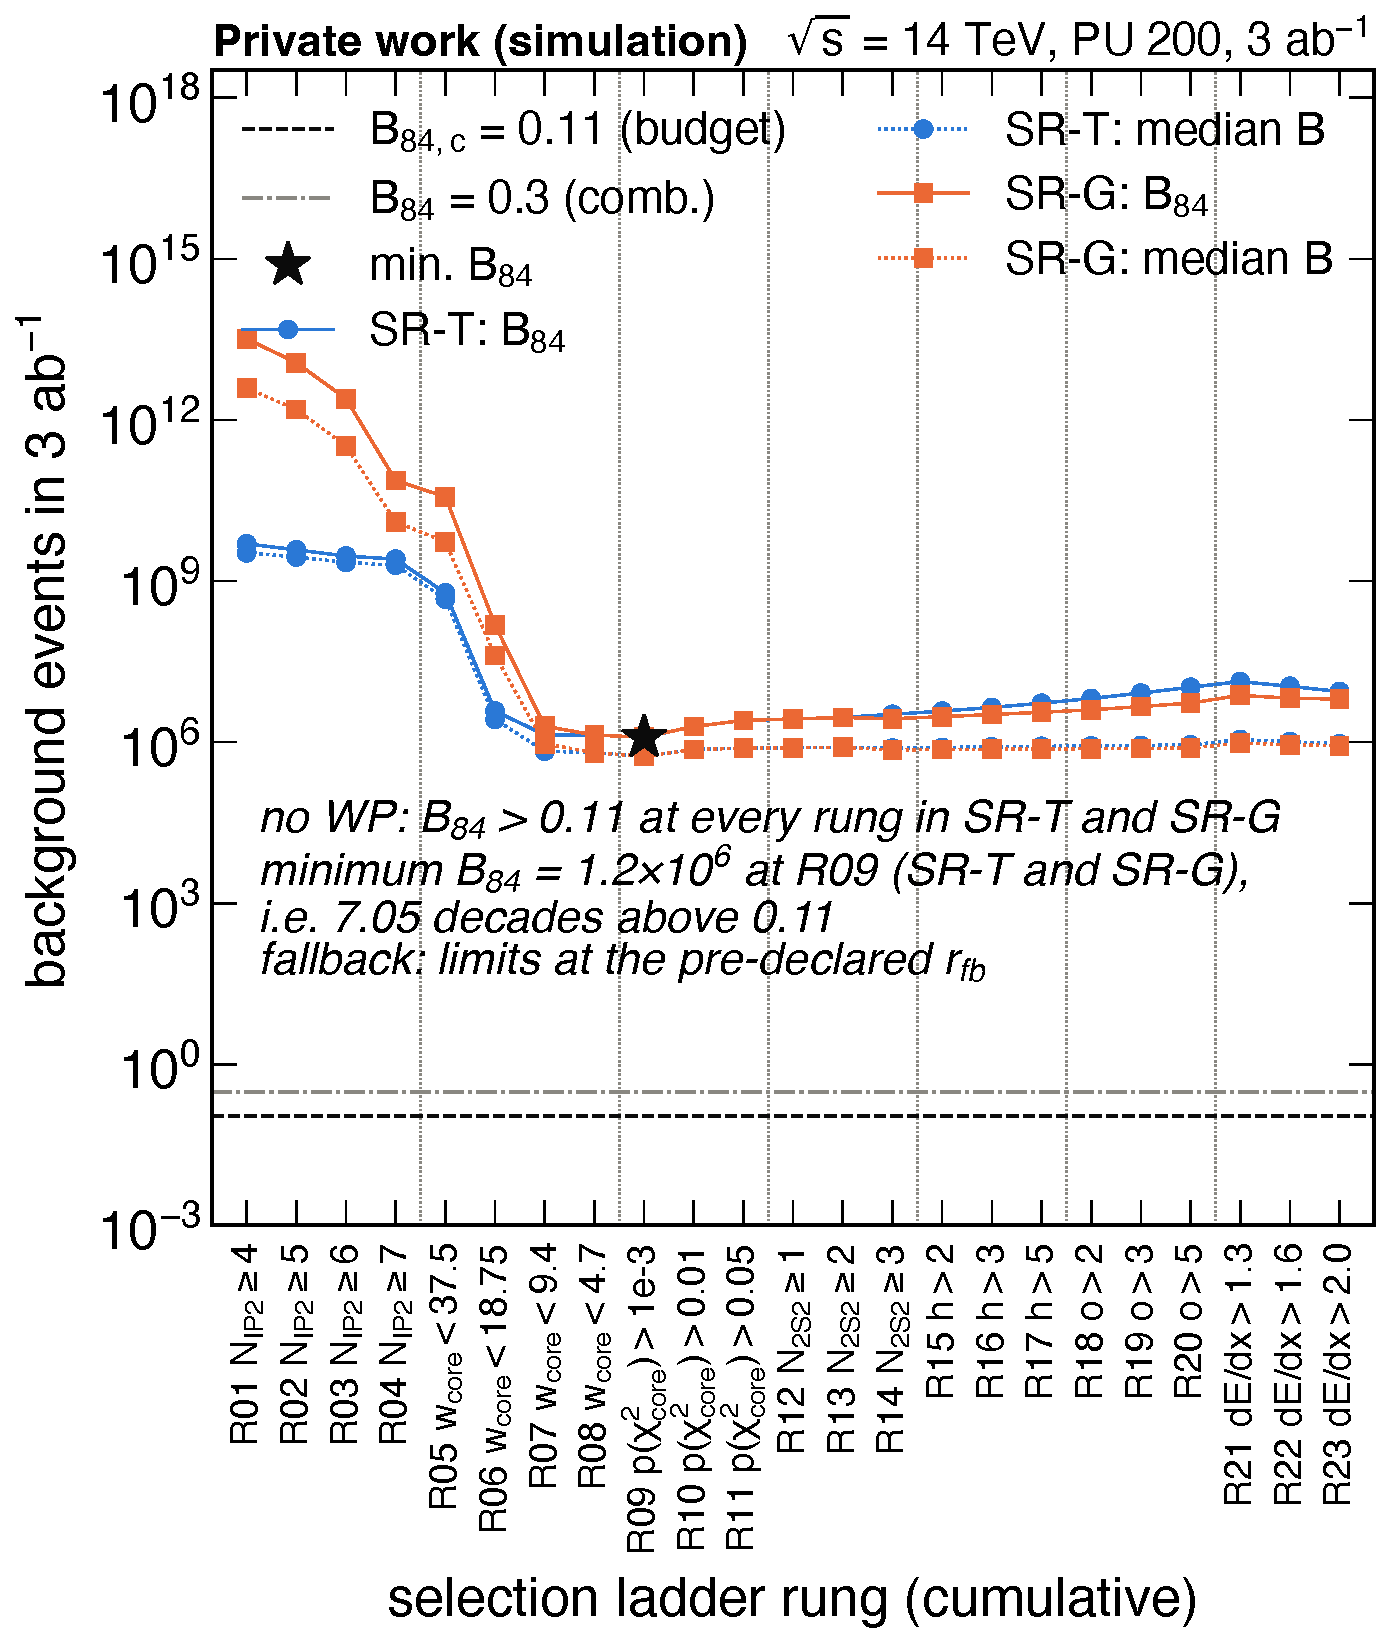
\includegraphics[height=0.37\linewidth]{figures/D3_bsum_vs_rung.pdf}\hspace{0.02\linewidth}
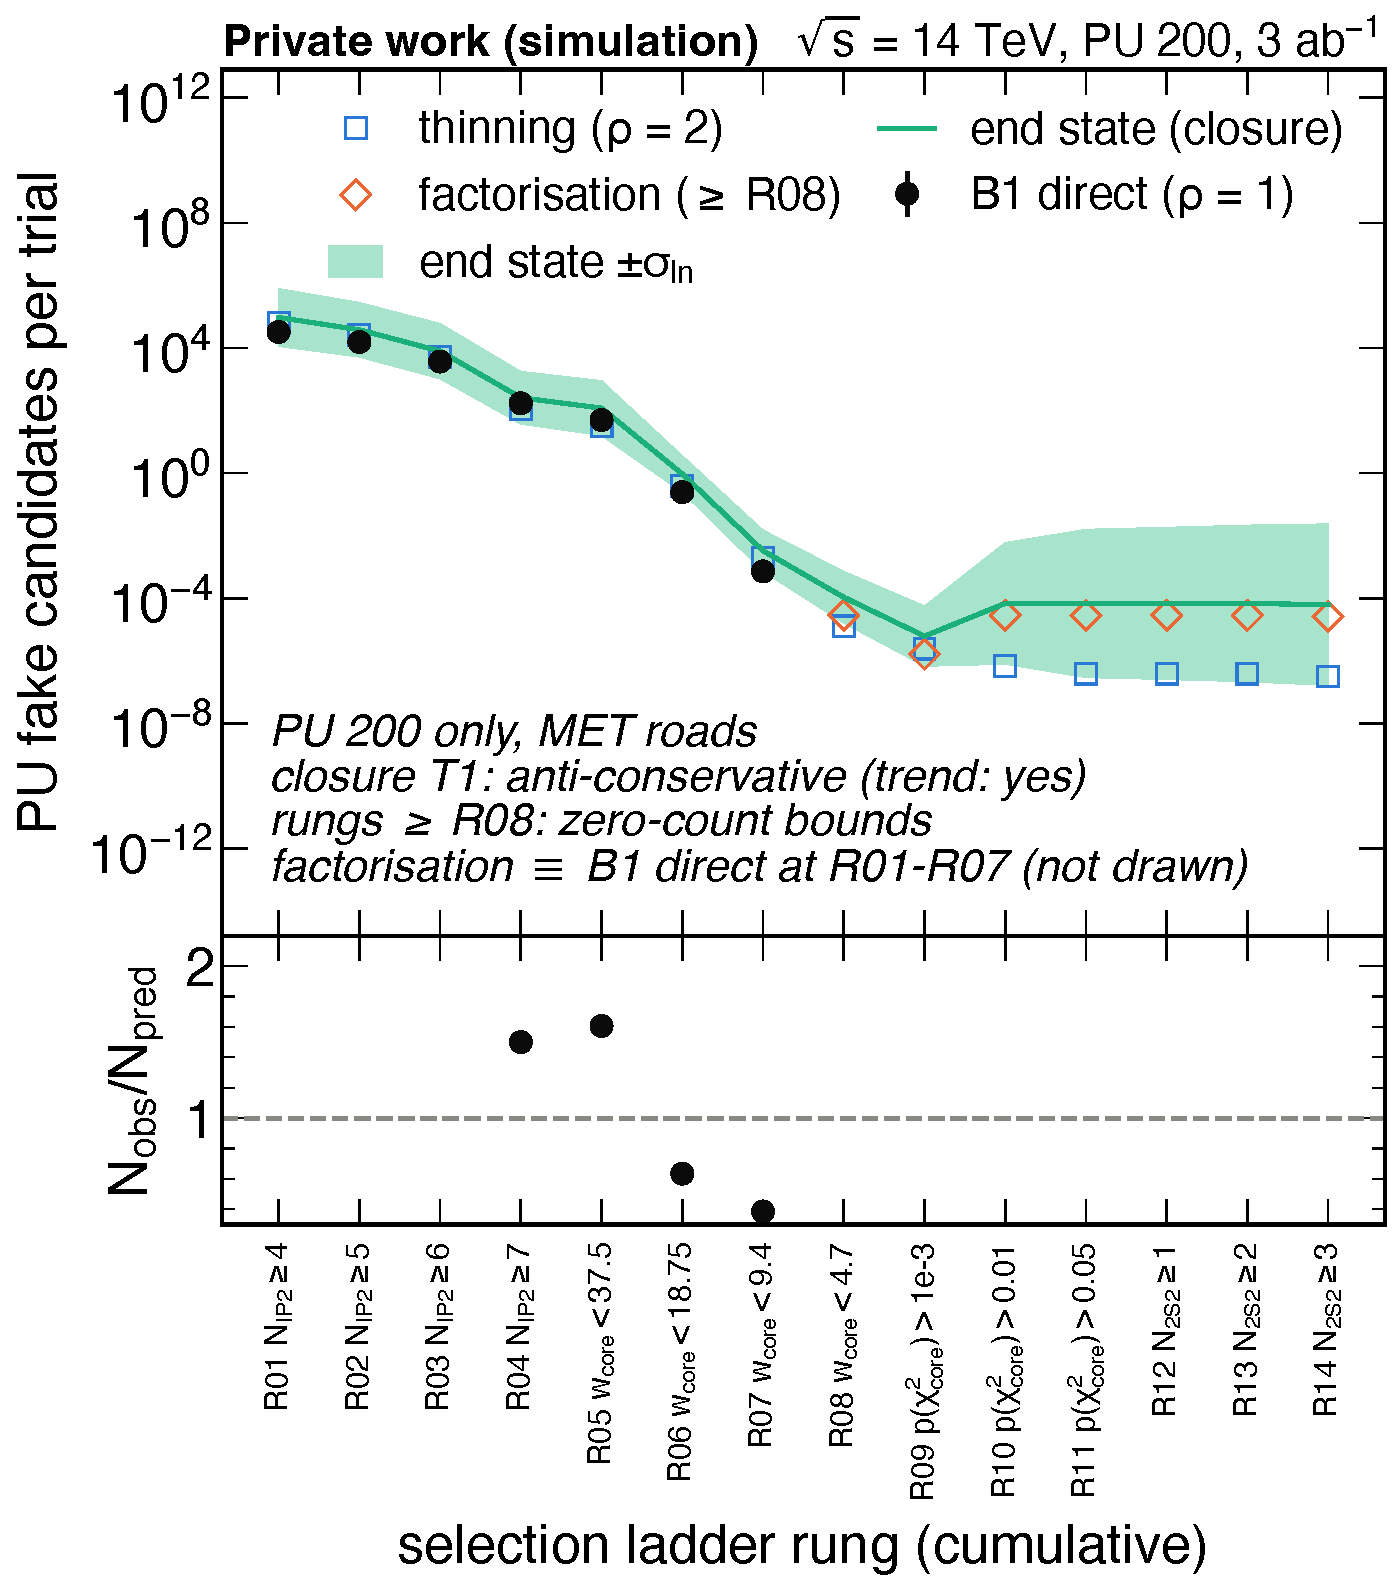
\includegraphics[height=0.37\linewidth]{figures/D4_pfake_extrapolation.pdf}
\caption{Background along the frozen ladder (detector level, PU 200, barrel). (Left) $\Nbkgeightyfour$ and the median
background in $3\abinv$ for SR-T and SR-G against the rung, with the per-category budget 0.11 and the combined 0.3; the
star marks the minimum, $1.2\times10^6$ at R09, 7.05 decades above the budget, so no working point exists. (Right)
Expected pile-up fake candidates per trial (one PU-200 event, one MET road): direct $\rho=1$ count, $\rho=2$ thinning,
the factorisation model where the direct count is zero, and the end state with the closure factor and its $\pm\sigma_{\ln}$
band; the lower panel shows the closure ratio $N_{\rm obs}/N_{\rm pred}$ at R04--R07. From R08 on the values are
zero-count bounds; the kink at R09--R10 comes from the switch between closure and extrapolation regimes.}
\label{fig:bkg}
\end{figure}

\paragraph{Why statistics alone cannot give a working point.} Each zero-count bound scales as $1/N$ with the sample
size. Bringing the leading bounded terms \emph{alone} to 0.11 would need $2.8\times10^9$ (PV pairs), $2.2\times10^9$
(decays in flight) and $8.4\times10^8$ ($Z(\nu\nu)$) events per sample, against 500--2000 now, and $\approx10^9$
$\rho=1$ trials for the pile-up term (now $4.8\times10^4$), whose irreducible trend and density uncertainty would still
require a median $\lesssim0.02$ (\EST{}). \textbf{The result is therefore limited by simulation statistics and by the
extrapolation uncertainty, not by a measured background}; a working point needs new handles or a data-driven background
estimate (Section~\ref{sec:concl}). Figure~\ref{fig:display} illustrates the difficulty: a pile-up-only fake can look as coplanar and as
non-helical in the transverse view as a quirk ribbon.

\begin{figure}[htbp]
\centering
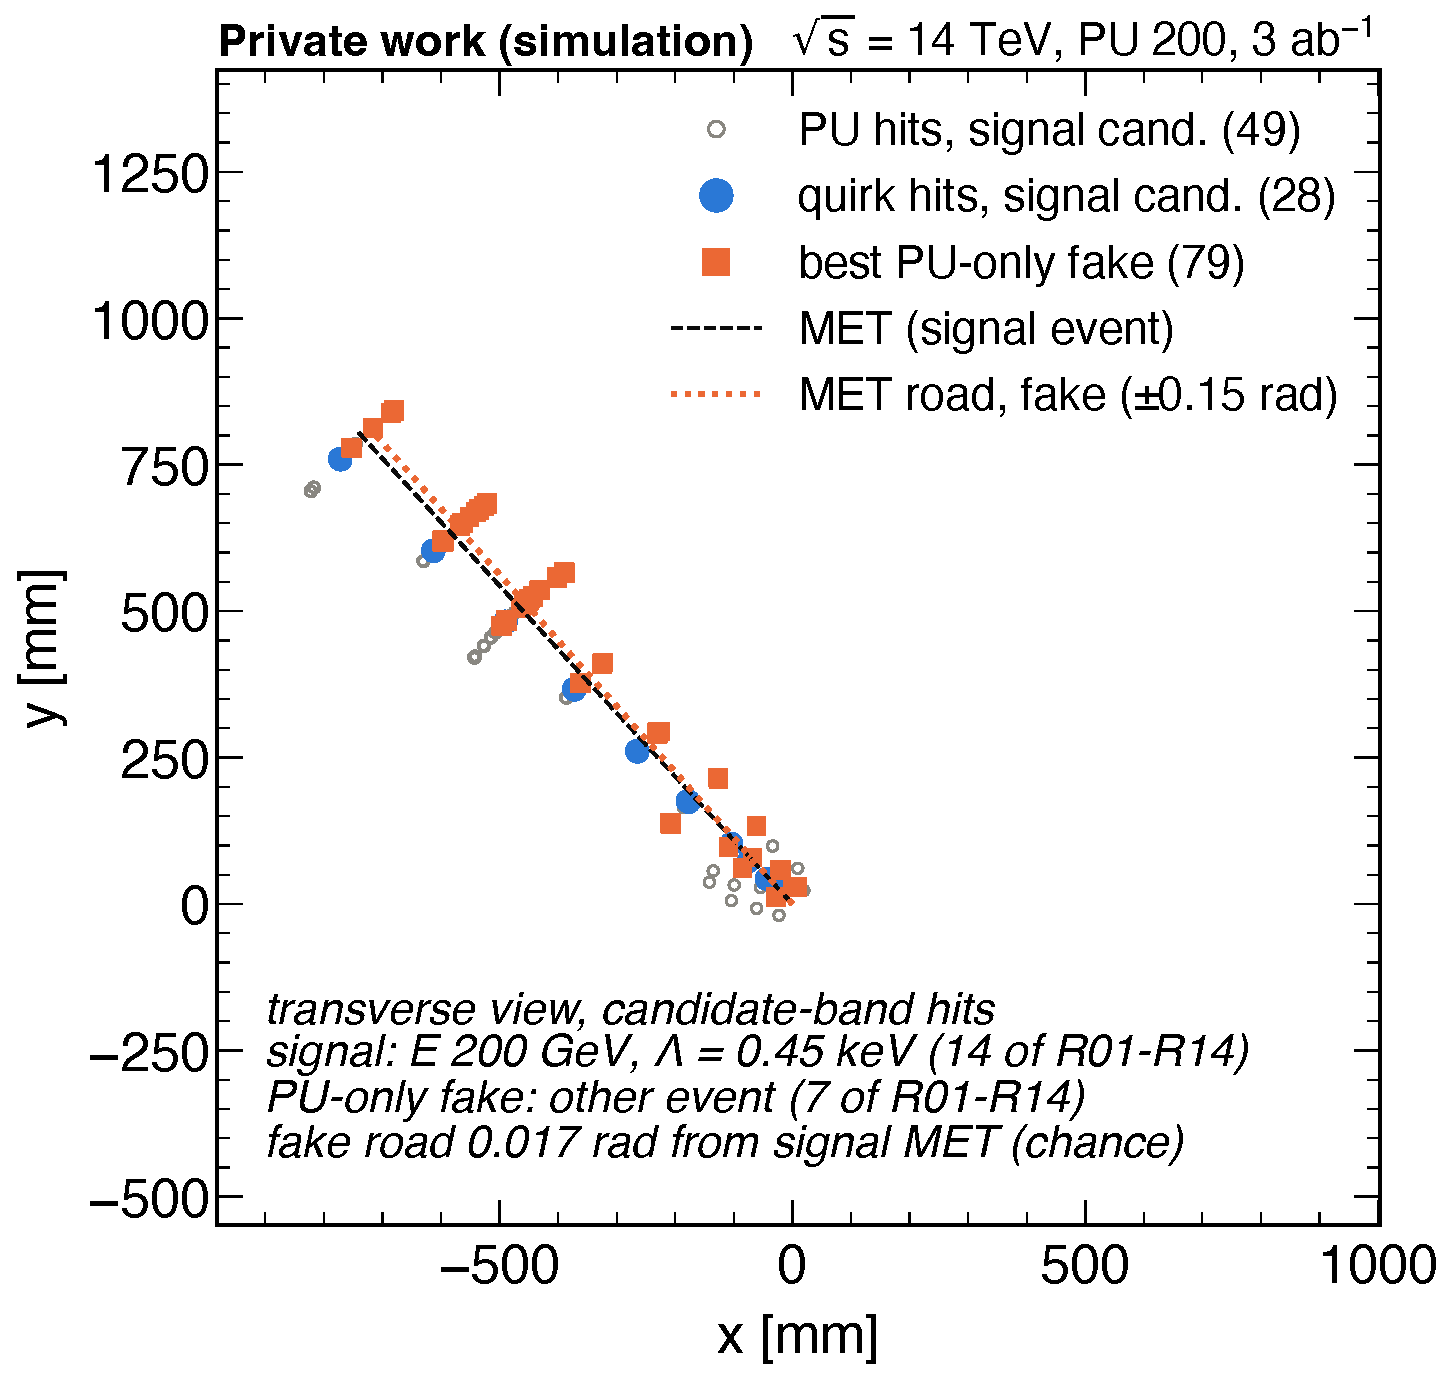
\includegraphics[height=0.32\linewidth]{figures/D11_event_display.pdf}
\caption{Transverse view of candidate-band hits at detector level (PU 200). Blue: quirk hits of a signal candidate ($E$ at
$200\GeV$, $\Lam=0.45\keV$, passing 14 of the rungs R01--R14), with the pile-up hits in its band (grey); orange: the best
pile-up-only fake of a different event (passing seven rungs), drawn in the same frame along its own MET road. Both lie along
a line through the vertex in this view; the fake fails the later width, core-$\chi^2$ and 2S rungs.}
\label{fig:display}
\end{figure}


\section{P2 results: working-point outcome, signal efficiency and fallback limits}\label{sec:results}

This section reports the detector-level outcome of the frozen rule, the signal efficiencies and the fallback limits. All
numbers are from the final, frozen analysis run (campaigns C1a, C1b, C2B and A2FC; \rep{acts/stage4/STAGE4_RESULTS.md},
machine-readable in \rep{data/acts_stage4/analysis/STAGE4_SUMMARY.json}). Everything is detector-level simulation in a
public-geometry model, barrel only; the acceptance factor is truth level.

\subsection{Working-point outcome}\label{sec:results:wp}
\textbf{No working point exists in either category.} $\Nbkgeightyfour>0.11$ already at R01 and at every rung after it;
the minimum is $1.23\times10^6$ at R09 in SR-T and SR-G (Section~\ref{sec:bkg:ladder}), and the best fallback column
(FB3) has $2.0\times10^6$ per category, $\approx4\times10^6$ combined, 7.1 decades above 0.3. By the frozen rule the
pre-defined fallback of Section~\ref{sec:strategy:fallback} therefore applies at every $(\mQ,\Lam)$: one admissible
selection per hypothesis, chosen from the frozen admissibility table and never optimised, with a non-zero log-normal
background. The fallback gives efficiencies, backgrounds and expected limits; it gives no background-free statement, no
discovery reach and nothing in the merged regime. Because the deep-rung backgrounds are zero-count bounds
(Section~\ref{sec:bkg:ladder}), the limits below measure the reach of this simulation set-up. They are conservative
with respect to simulation statistics and would move in proportion to the bounds with more simulated events, but the
untested rung factorisation (Section~\ref{sec:bkg:closure}) can bias them in either direction.

\subsection{Signal efficiency}\label{sec:results:eff}
The efficiency counts an event if a candidate passes the selection, has $f_{\rm CKF}<0.2$ and is signal-matched by the
pre-declared definition of Section~\ref{sec:strategy:trig}; the denominator is the template half with $|\eta_{\rm
pair}|<2.5$, 180--200 events per point. The barrel-only selection caps it at $\approx0.3$.

\paragraph{Finder efficiency without pile-up (V4-3: partial).} The pre-registered check V4-3 asked for a finder efficiency
$\ge0.9$ at 1--5\,keV without pile-up. With pairs in the barrel ($|\eta_{\rm pair}|<1$) and a match ``some candidate holds
$\ge50\%$ of the quirk hits'' that was defined only after the first comparison failed (a post-hoc reading), the finder
reaches 0.90--0.97 at 1.5--2\,keV for all five (species, mass) points ($\Etil$ 500: 2\,keV only), but 0.75--0.90 at 1\,keV, 0.83--0.97 at 3\,keV and
0.58--0.84 at 5\,keV; with the counting rung R04 also required it is 0.64--0.77 at 1.5--2\,keV. V4-3 is therefore
\emph{partial}. The losses are understood: R04 needs two crossings on every one of the seven IT and PS barrel layers, so a
single merged pair kills it at high $\Lam$; the seed needs an opening of at least 1\,mrad; and the CKF removes quirk hits.

\paragraph{Efficiency at pile-up 200.} Figure~\ref{fig:eff} shows the efficiency at the fallback selection $r_{\rm fb}$
and along the ladder. At R04 it is 0.085--0.31 at $1$--$5\keV$; at the fallback it is 0--0.080 over all 40 points (maximum
0.080 at $E$ 500 at 2 and $5\keV$ and $\Etil$ 500 at $5\keV$), and zero in both categories at seven points ($E$
500/1000/1500 at $0.45\keV$, $E$ 1500 at $0.6\keV$, $\Etil$ 500 at $\le0.85\keV$). The SR-T share is typically 30--70\% (range 0--100\%) of
$\Eff(r_{\rm fb})$ at $\mQ\ge500\GeV$ and $\le27\%$ at $200\GeV$. At $\Lam\gtrsim2\keV$ the efficiency with pile-up is
\emph{above} the one without: pile-up hits complete the layer count where the quirk pair has merged, so the high-$\Lam$
candidates are partly pile-up-assisted.

\paragraph{Full-chain revert and its systematic.} The fast signal path digitises quirk hits outside ACTS and never passes
them through the CKF. Under the pre-registered rule, the nine points where more than 5\% of quirk hits were taken by CKF
tracks without pile-up ($\{E\,200,500,1000,1500\}\times\{3,5\}\keV$ and $\Etil$ 500 at $5\keV$) were re-run through the
full chain (A2FC; same rows and seeds, pile-up measurement noise re-drawn). At R04, the only genuinely paired rung, the full
chain is 5--30\% lower; summed over eight of the nine points the loss is $\times0.83$ at R04 (84 against 20 discordant
events, $p\approx1.6\times10^{-10}$) and $\times0.87$ at $r_{\rm fb}$, attributed to CKF hit stealing (confirmed for one
event, inferred for the aggregate). At $E$ 500, $3\keV$ the full chain cut $\Eff$(FB3) from 0.145 to 0.055 ($11/200$, 68\%
CP $[0.039,0.076]$); the investigation found no bug and attributes the drop to statistics, because re-drawing the noise
flips 25--50\% of the passing events at R08--R14 (global $p\approx10^{-4}$--$10^{-3}$; a conclusion by exclusion). The full
chain is the reference at the nine points; the 31 others stay on the fast path and may overestimate $\Eff$ by up to
$\approx1/0.87$ (\EST{}, not applied).

\begin{figure}[htbp]
\centering
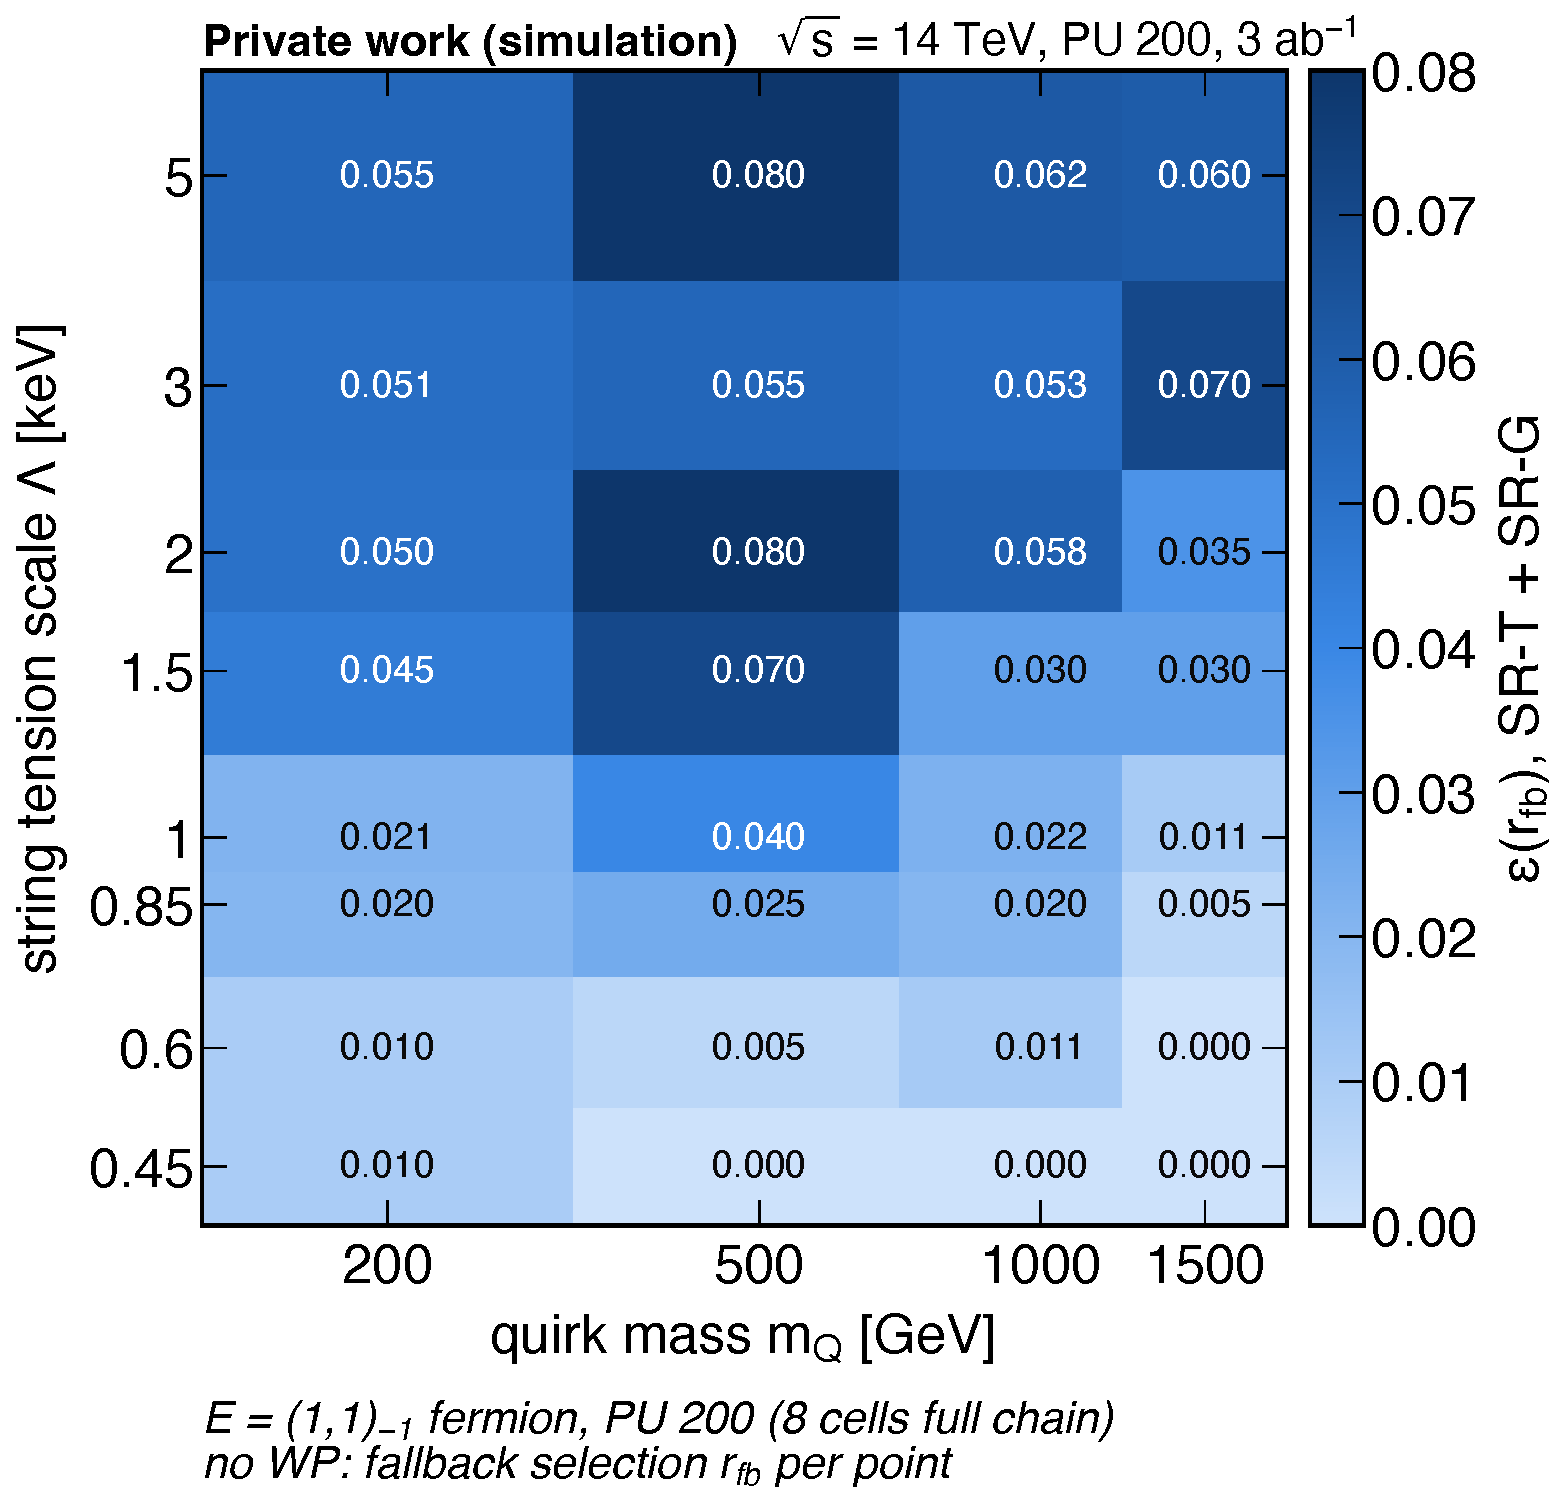
\includegraphics[height=0.37\linewidth]{figures/D1_eps_map_rfb.pdf}\hspace{0.02\linewidth}
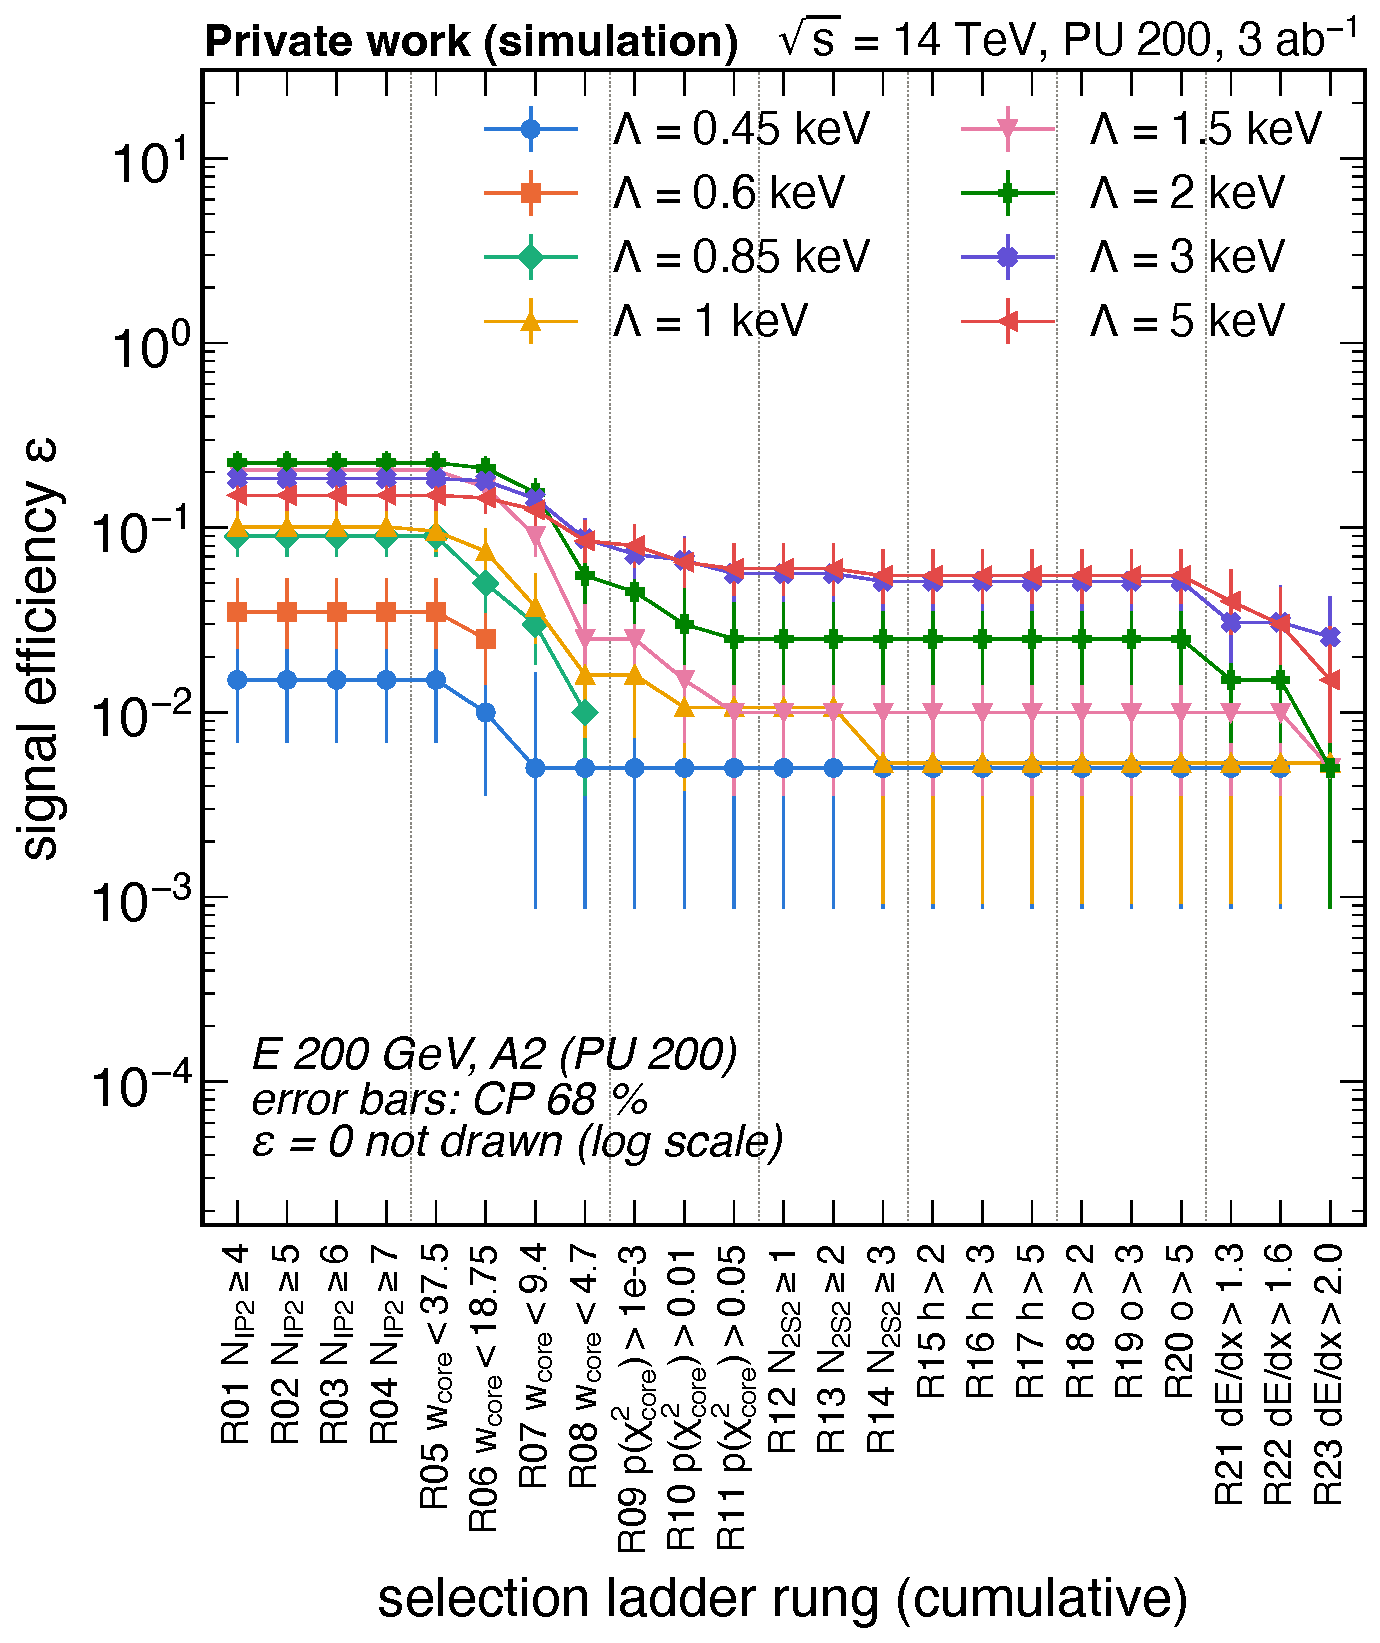
\includegraphics[height=0.37\linewidth]{figures/D2_eff_vs_rung_F200.pdf}
\caption{Signal efficiency at detector level (PU 200, barrel, fermion $E$). (Left) Efficiency at the pre-declared fallback
selection $r_{\rm fb}$ (SR-T + SR-G) on the $(\mQ,\Lam)$ grid; eight cells at 3 and $5\keV$ use the full ACTS chain
(the ninth full-chain point, $\Etil$ 500 at $5\keV$, is not in this map), the others the fast signal path. (Right) Efficiency along the 23 cumulative rungs for $\mQ=200\GeV$ at each $\Lam$, with
68\% Clopper--Pearson errors (zero values not drawn). The efficiency stays below $\approx0.08$ at the fallback: the
barrel selection caps it at $\approx0.3$ and the deep cuts cost the rest.}
\label{fig:eff}
\end{figure}

\subsection{Fallback limits}\label{sec:results:limits}
The expected 95\% CL upper limit on the number of signal events in the trigger and preselection acceptance uses the
two-category counting likelihood of Section~\ref{sec:strategy:fallback} with hybrid-CL$_s$ toys (primary). It is
converted to a limit on the inclusive cross section, $\sigma_{95}=\mu_{95}/(Lf_{200}A)$, with the tail fraction $f_{200}$
and the truth-level acceptance $A$ of Eq.~\eqref{eq:effchain} (Table~\ref{tab:acc}), and compared with
$N_{\rm exp}=\sigma_{\rm norm}f_{200}LA$, so that $\sigma_{95}/\sigma_{\rm norm}=\mu_{95}/N_{\rm exp}$.
Figure~\ref{fig:limits} shows the limits for $\mQ=200\GeV$ against $\Lam$ and against $\mQ$ at $\Lam=1.5\keV$, and
Figure~\ref{fig:excl} in Section~\ref{sec:bounds} the full grid.

\textbf{No point is excluded.} The best expected limit is $\sigma_{95}/\sigma_{\rm norm}=\mu_{95}/N_{\rm exp}=790$ at $E$
200, $\Lam=1.5\keV$ ($r_{\rm fb}=$ FB2, $\Eff=9/200=0.045$, 68\% CP $[0.030,0.065]$, 95\% CP $[0.021,0.084]$; $\mu_{95}=1.25\times
10^7$ events, toy $\pm1\sigma$ band $[8.6\times10^5,1.9\times10^8]$, asymptotic/toys 1.05; $N_{\rm exp}=1.58\times10^4$,
$S=710$, $\sigma_{95}=1.7\times10^5\fb$ against $\sigma_{\rm norm}=219\fb$). The statistical uncertainty of $\Eff$ moves the
ratio by a factor $\approx1.5$ either way at 68\% CL; even the 95\% CP upper efficiency gives $\approx420$, and an
exclusion would need $\Eff\approx36$, which is impossible. With the full-chain systematic of Section~\ref{sec:results:eff}
the ratio becomes $\approx910$--950 (\EST{}, not applied). The second-best point is $E$ 200 at $2\keV$ (820); all others lie
between $2.3\times10^3$ ($E$ 200, $1\keV$) and $6.0\times10^7$ ($E$ 1500, $0.85\keV$). The best ratio per mass is
$1.3\times10^4$ ($E$ 500), $3.8\times10^5$ ($E$ 1000), $3.8\times10^6$ ($E$ 1500) and $2.8\times10^5$ ($\Etil$ 500), all at
$3\keV$; 33 of 40 points have a limit and seven have $\Eff=0$. Even with zero background only 20 of the 40 points would
have $S\ge3$ selected events ($E$ 1500 at most 0.3). The $5\sigma$ discovery yields, where computed, are
$1.9\times10^4$--$2.4\times10^8$ times the prediction. These ratios include $f_{200}$; an earlier version of the
analysis omitted it and quoted values $1/f_{200}=6$--21 times smaller (erratum in \rep{STAGE4_RESULTS.md}).

\begin{table}[htbp]
\centering
\small
\caption{Tail fraction $f_{200}$, truth-level acceptance of the tail sample (Stage 3, template half) and predicted yield
$N_{\rm exp}=\sigma_{\rm norm}f_{200}\,3\abinv\,A$ ($N_{\rm IC}=2$), used to convert the detector-level limits
(\rep{STAGE4_RESULTS.md} \S4.4); $A_{\rm incl}=f_{200}A$. $\Eff_{\rm PV}=1$ (not modelled).}
\label{tab:acc}
\begin{tabular}{lccccccl}
\toprule
point & $f_{200}$ & $\Eff_{\rm fid}$ & $\Eff_{\rm trig}$ & $\Eff_{\rm presel|trig}$ & $A$ & $A_{\rm incl}$ & $N_{\rm exp}$\\
\midrule
$E$ 200 & 0.0476 & 0.847 & 0.90--0.91 & 0.65--0.66 & 0.49--0.50 & 0.024 & $1.55$--$1.58\times10^4$\\
$E$ 500 & 0.104 & 0.830 & 0.92--0.93 & 0.74--0.75 & 0.57 & 0.059--0.060 & $1.08$--$1.09\times10^3$\\
$E$ 1000 & 0.146 & 0.816 & 0.93--0.94 & 0.84--0.85 & 0.64--0.65 & 0.093--0.095 & 55--56\\
$E$ 1500 & 0.169 & 0.752 & 0.94--0.95 & 0.81--0.82 & 0.58 & 0.098--0.099 & 4.2\\
$\Etil$ 500 & 0.1135 & 0.826 & 0.93 & 0.71--0.72 & 0.55 & 0.062--0.063 & 85--86\\
\bottomrule
\end{tabular}
\end{table}

\begin{figure}[htbp]
\centering
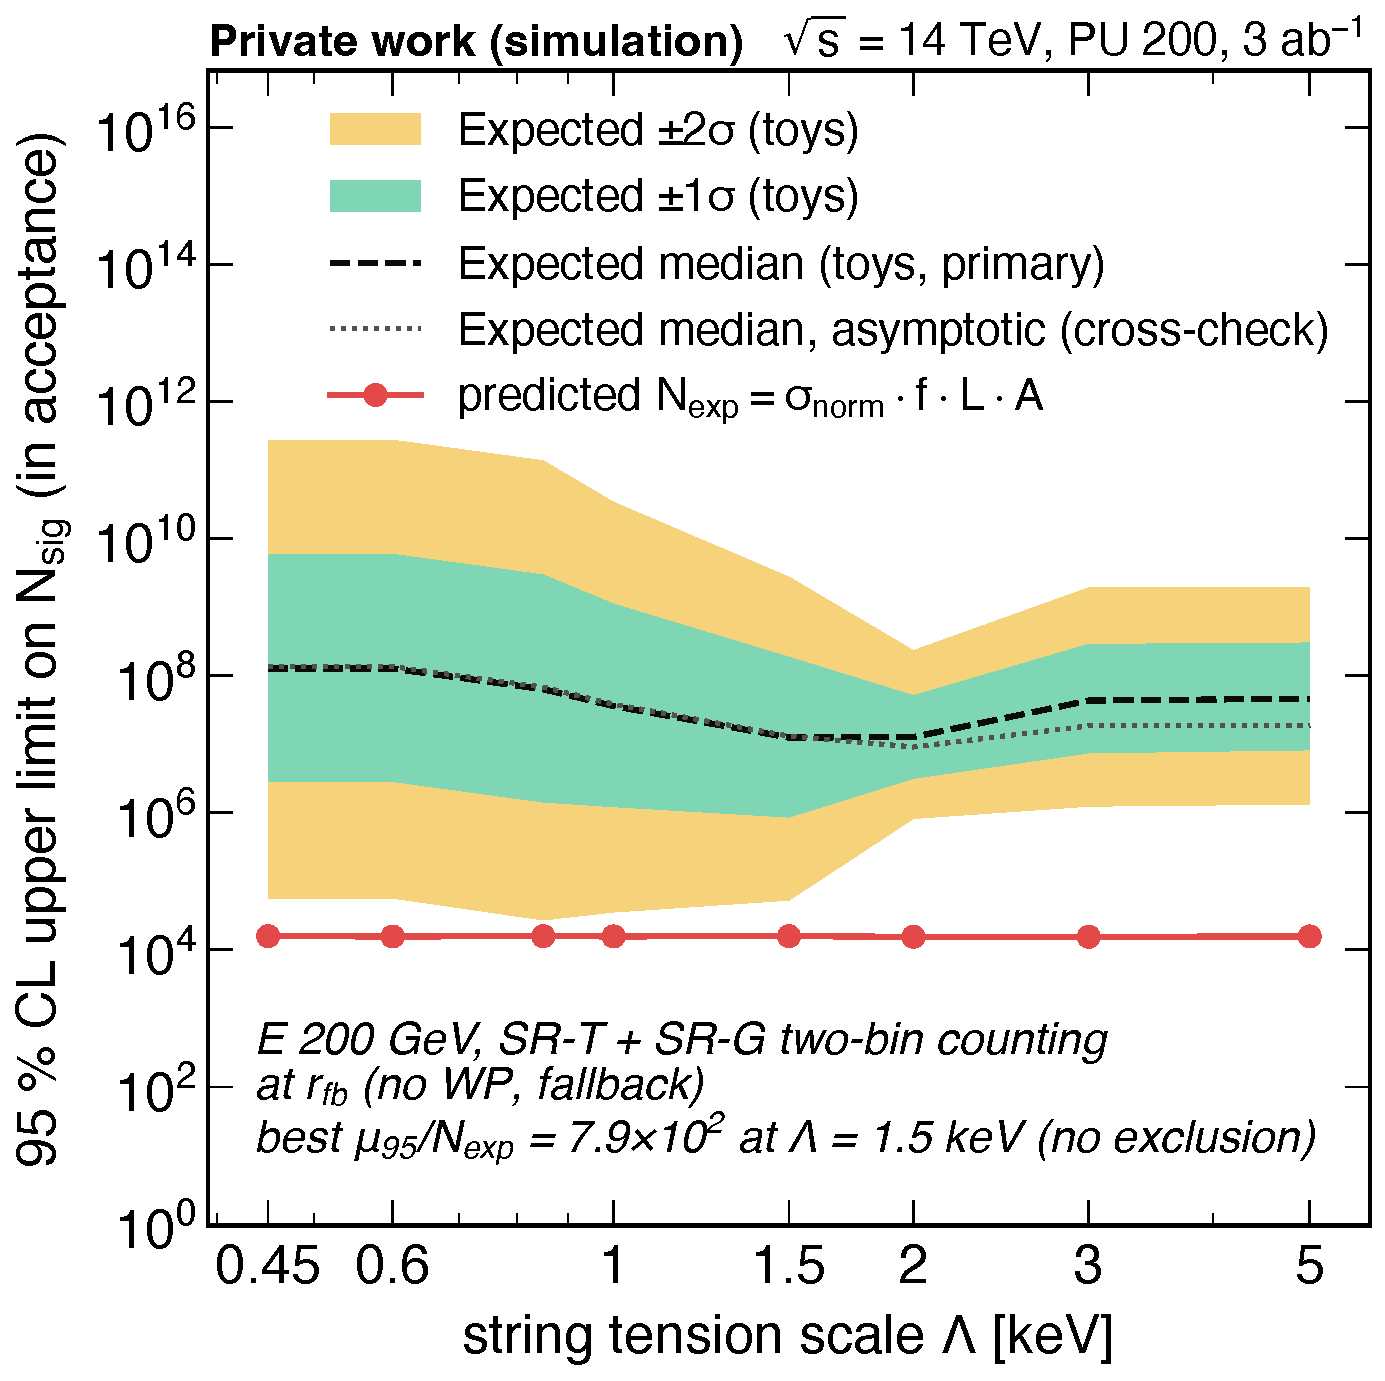
\includegraphics[height=0.37\linewidth]{figures/D5_limit_mu_vs_lambda_F200.pdf}\hspace{0.02\linewidth}
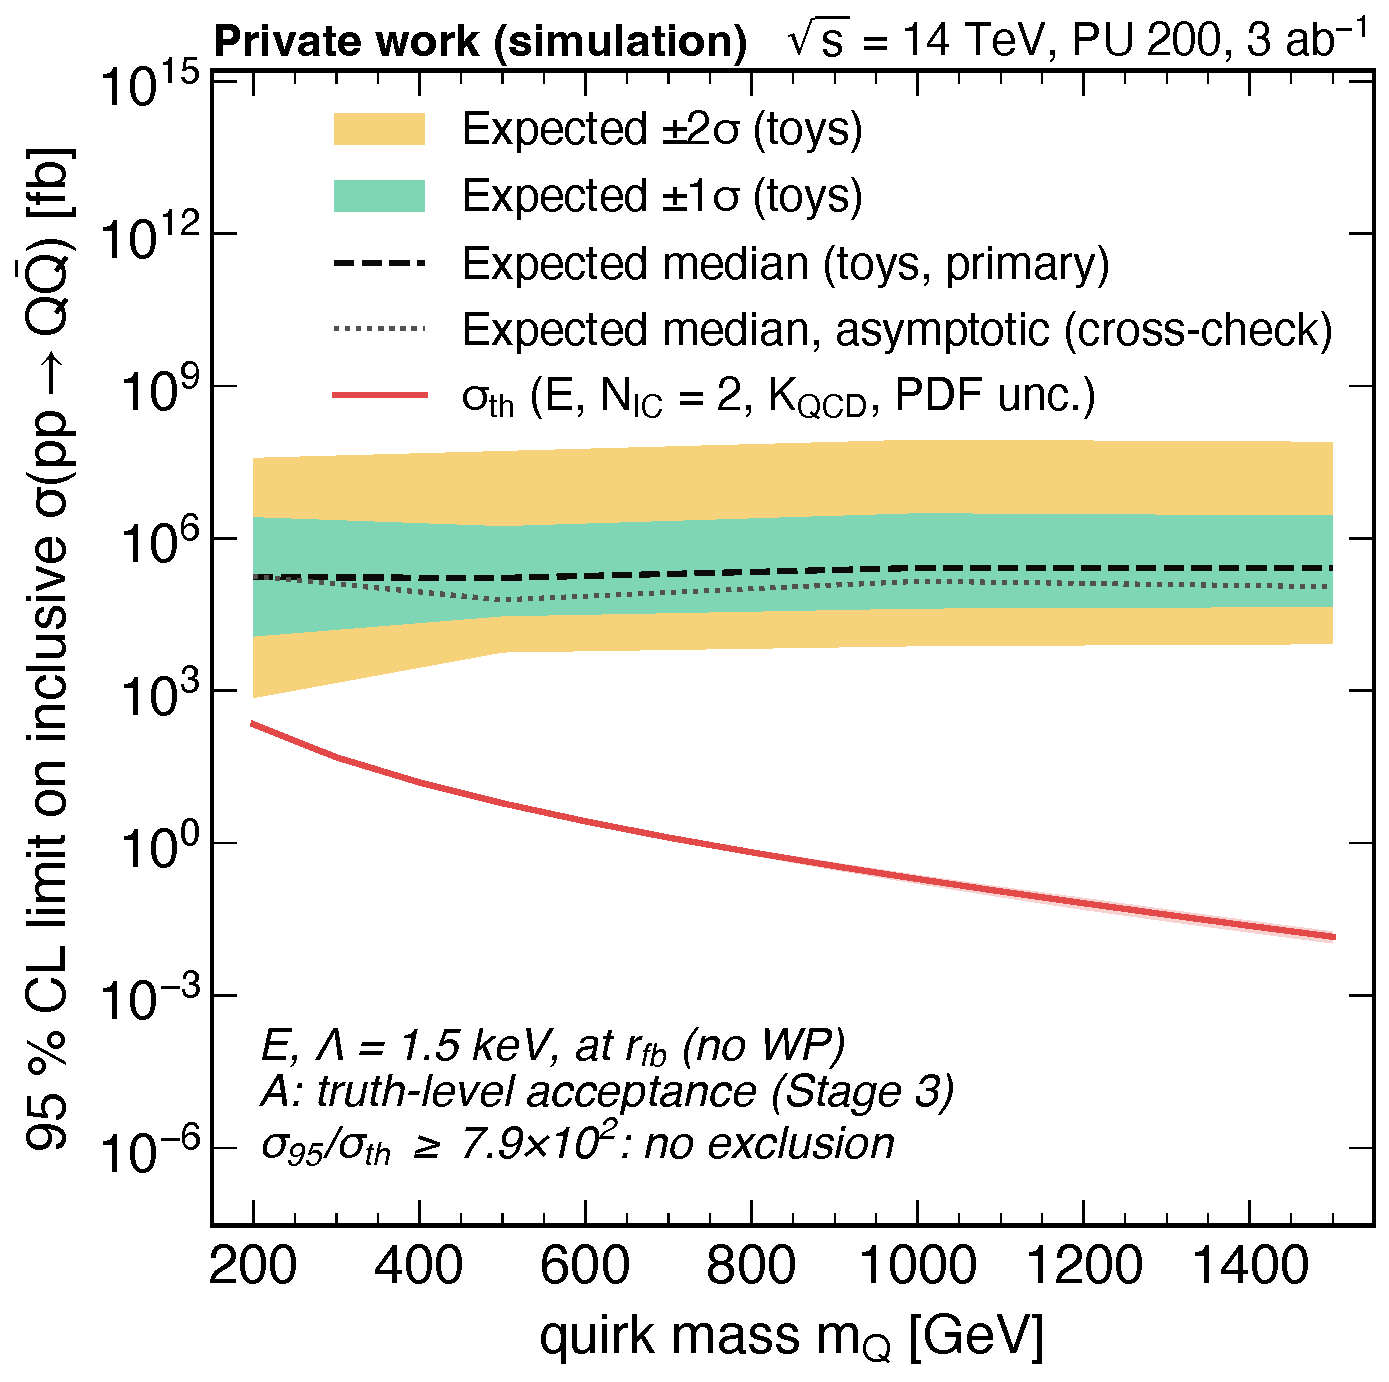
\includegraphics[height=0.37\linewidth]{figures/D6_limit_xsec_vs_m_L1p5.pdf}
\caption{Expected 95\% CL limits at the fallback selection (detector level; acceptance truth level; no working point).
(Left) Limit on the number of signal events in the acceptance for $E$ at $200\GeV$ against $\Lam$, with toy $\pm1\sigma$ and
$\pm2\sigma$ bands (primary), the asymptotic median (cross-check) and the predicted yield. (Right) Limit on the inclusive cross section
against $\mQ$ at $\Lam=1.5\keV$ with the predicted cross section ($\sigma_{\rm norm}$ with $K_{\rm QCD}$, labelled $\sigma_{\rm th}$; $N_{\rm IC}=2$). The median limit is at least 790 times
the prediction everywhere: nothing is excluded. The deep-rung background central values are zero-count simulation bounds.}
\label{fig:limits}
\end{figure}

\subsection{Systematic uncertainties}\label{sec:results:syst}
The limits carry the following uncertainties, each entering as a log-normal nuisance or, where stated, only as a
reported variation. (i) \emph{Signal normalisation}: $\pm5\%$ on $\sigma_{\rm norm}$ (Section~\ref{sec:model:xsec}) and
$+12$--15\%/$-11$--13\% on the tail fraction $f_{200}$ (Section~\ref{sec:model:syst}); neither is propagated into
$\mu_{95}/N_{\rm exp}$, and both are small against the factor $\ge790$.
(ii) \emph{Background}: per term, statistical, extrapolation-model, density-normalisation and normalisation components
(Section~\ref{sec:strategy:rule}); at the headline point the SR-G background is dominated by the zero-count PV-pair bound with
$\sigma_{\ln}\approx1.5$. (iii) \emph{Efficiency}: the binomial uncertainty above and the full-chain systematic (not
applied). The MET resolution (25\,GeV, variations 15/35\,GeV), the trigger turn-on ($\pm25\GeV$ on its 50\% point) and
the PV-identification efficiency are parametrised assumptions (\UNV{}) and are not propagated to the final limits.
(iv) \emph{Statistical treatment}: SR-T and SR-G are treated as uncorrelated although single-interaction and SM terms
enter both identically. This is anti-conservative where both categories carry signal (23 of the 33 points with a limit),
but irrelevant at the headline point, where the SR-T efficiency is zero. None of these can
turn the null result into an exclusion: that would need a background lower by many orders of magnitude.

\section{Measuring the quirk mass and the confinement scale (P2)}\label{sec:mlam}

If a quirk signal were seen, the next questions would be its mass $\mQ$ and the string scale $\Lam$. The hit pattern
depends on them through a few combinations: $\lzero=\mQ/\Lam^2$ sets the oscillation length (Eq.~\eqref{eq:lmax}),
$\epsB\propto B/\Lam^2$ the B-field thickness (Eq.~\eqref{eq:law}), and the velocities, which depend on $\mQ$ through the
production kinematics, set the number of oscillations, the hit delays and the ionisation. This section first gives the
truth-level handles from Stage~3, which define what a detector-level measurement should be compared with, and then the
detector-level handles.

\subsection{Truth-level handles}\label{sec:mlam:truth}
The truth-level handles show what information the hit pattern carries before resolution, pile-up and reconstruction
remove part of it; each detector-level handle of Sections~\ref{sec:mlam:det} and~\ref{sec:mlam:mass} is compared with
its truth-level counterpart.
Figure~\ref{fig:edges} shows the main truth-level handles (template half of the Stage-3 sample, $|\eta_{\rm pair}|<2.5$,
smeared vertex, field and nominal material; \rep{sim/stage3/results/P2.json}).
\begin{itemize}
\item \textbf{A continuous $\Lam$ handle.} The median separation of the two quirks in the IT, $\sepIT$, scales as
  $\Lam^{-2}$ from 1 to $30\keV$ at every (species, mass) point (log-log slopes $-1.985$ to $-2.022$, each $\pm0.02$--0.04): it
  measures $\lzero=\mQ/\Lam^2$, with $\sepIT/\lmax\approx0.5$--0.6 above $1\keV$. For $E$ at $1000\GeV$ it falls from
  $38.5\mm$ at $1\keV$ to $9.3\mm$ at $2\keV$, $0.37\mm$ at $10\keV$ and $95\um$ at $20\keV$.
\item \textbf{Breaking the $(\mQ,\Lam)$ degeneracy} (truth level, \EST{}). Below $\Lcross(\mQ)$ ($1.2$--$1.9\keV$)
  the thickness is dominated by the B-field part, which depends on $\Lam$ only and is flat in $\mQ$
  (Section~\ref{sec:p1}), while $\sepIT$ measures $\mQ/\Lam^2$; at truth level the two together would separate $\mQ$
  and $\Lam$ without using the recoil. Above $\Lcross$ the thickness is set by multiple scattering and depends on
  $\mQ$. The number of tracker hits, the maximum hit delay and the fraction of pairs that do
  not turn around inside the tracker are flat in $\Lam$ and carry $\mQ$ through the velocities.
\item \textbf{Edges.} The efficiency of a coplanarity search is bounded in $\Lam$ by scales of the string
  (Fig.~\ref{fig:edges}): (i) $\Nosc=1$ at $0.28$--$0.33\keV$, independent of $\mQ$; (ii) the median $\lmax$ equals the IT
  radius at $0.43\to0.78\keV$ ($E$, $200\to1500\GeV$) and $0.59\to0.94\keV$ ($\Etil$); (iii) the median truth thickness
  (field and material) reaches $100\um$ at $0.47$--$0.55\keV$, flat in $\mQ$, the only edge tied to $\epsB$; (iv) at high
  $\Lam$ the two quirks merge into one hit: half of the pairs have an IT separation below $100\um$ at $12.8\to20.4\keV$
  ($E$) and $17.7\to25\keV$ ($\Etil$). The median $\lmax=100\um$ threshold ($16\to30\keV$ for $E$) is the same quantity
  as (ii) at another threshold: since $\lmax\propto\Lam^{-2}$, the two thresholds differ by the fixed ratio
  $\sqrt{\RIT/100\um}=\sqrt{1465}=38.2$. The $\mQ$ dependence of the $\lmax$ edges is
  $d\ln\Lam/d\ln\mQ=0.249\pm0.019$, half of the naive $\sqrt{\mQ}$ scaling, because heavier pairs are produced with
  smaller $\gst$.
\item \textbf{Edge systematics.} Varying $\lmax$ by $\pm5\%$, QED radiation, scales, PDFs, the merging scale and the
  material by $\times0.5$/$\times2$ moves the edges by a median of 2.3--5.2\% per edge type and at most 8.1\%; these are
  noise-limited upper bounds (\EST{}).
\end{itemize}

\begin{figure}[htbp]
\centering
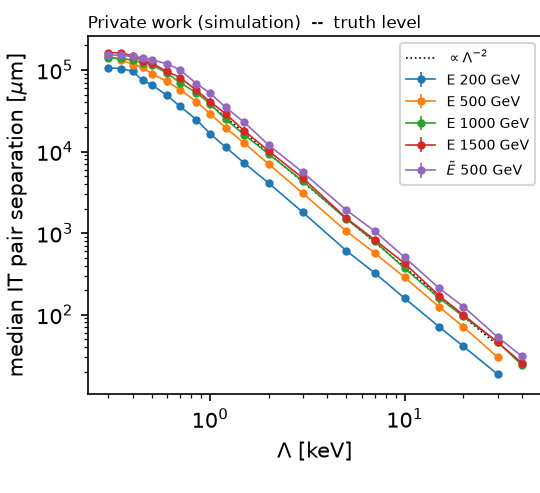
\includegraphics[height=0.37\linewidth]{figures/S3_p2_sepIT.png}\hspace{0.02\linewidth}
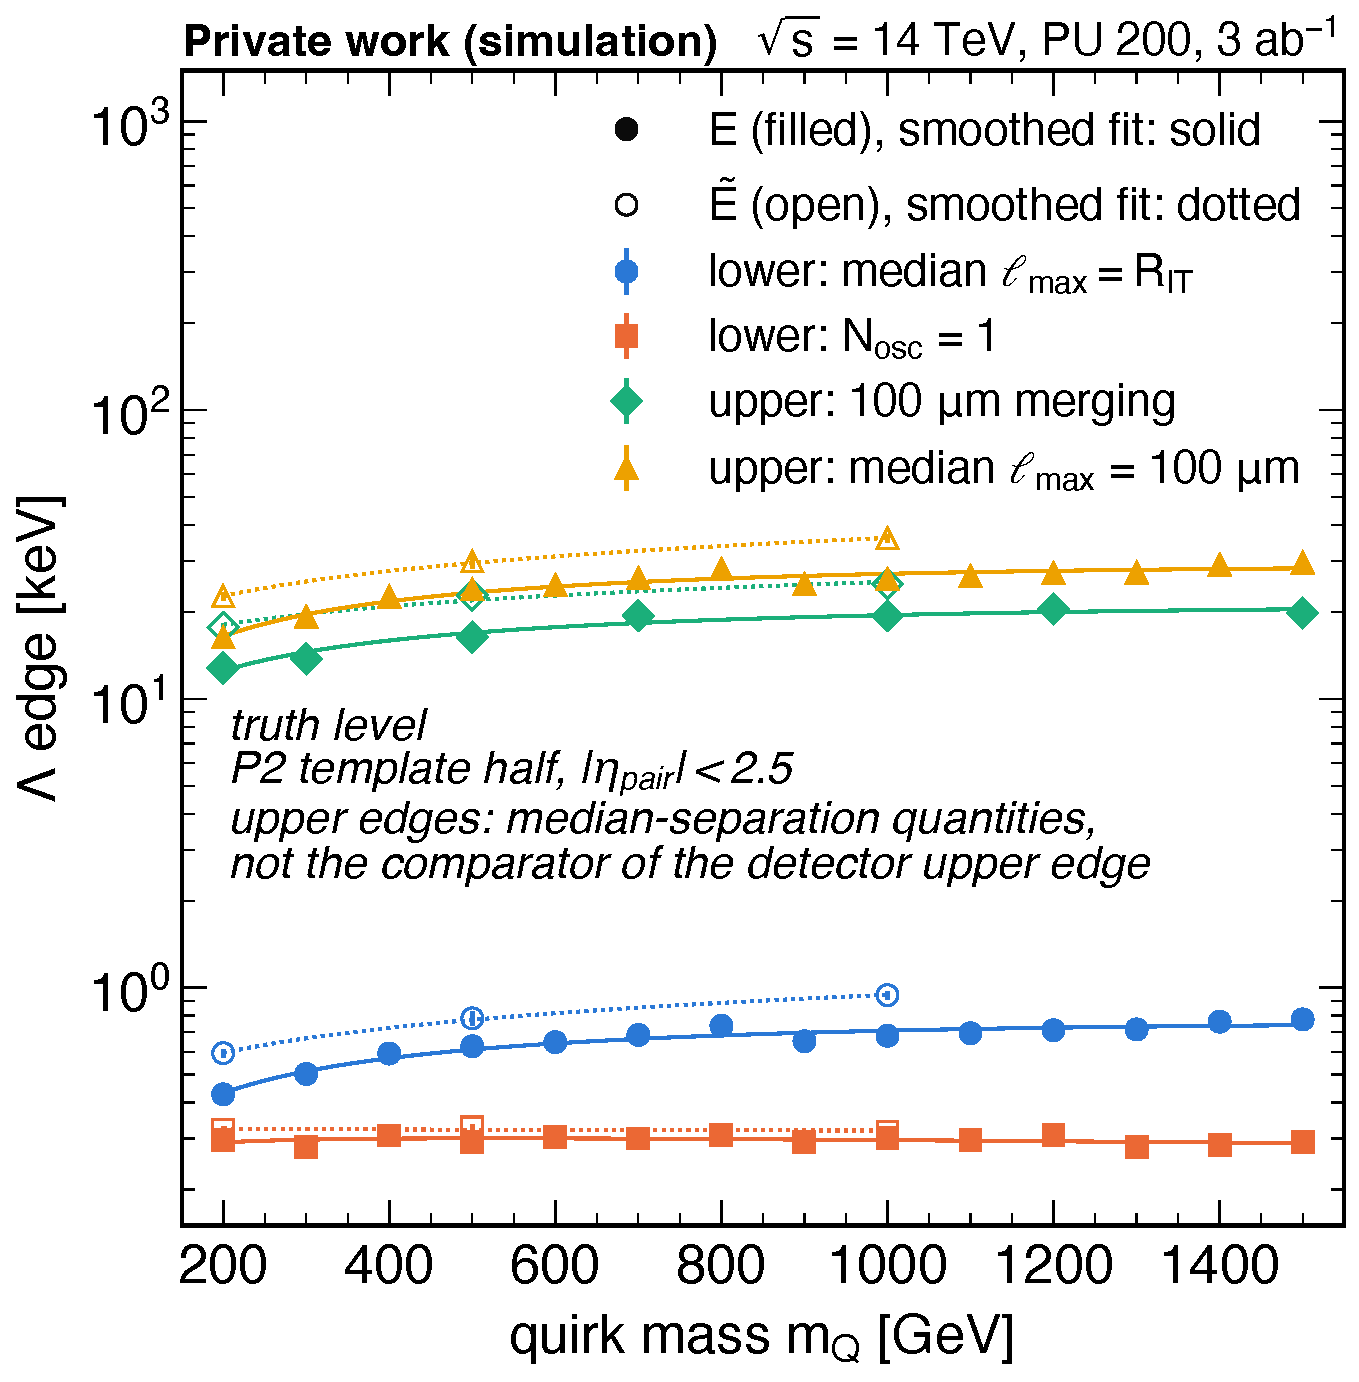
\includegraphics[height=0.37\linewidth]{figures/T4_truth_edges_vs_mass.pdf}
\caption{Truth-level P2 handles (Stage 3, template half, $|\eta_{\rm pair}|<2.5$, field and nominal material; no pile-up,
no resolution). (Left) Median separation $\sepIT$ of the two quirks in the IT against $\Lam$ for five (species, mass)
points (dotted: $\propto\Lam^{-2}$; one panel of the Stage-3 diagnostic figure \rep{sim/stage3/figures/p2_observables.png}):
it follows $\Lam^{-2}$ and so measures $\mQ/\Lam^2$. (Right) $\Lam$ edges against the quirk mass (filled markers and
solid fits: $E$; open markers and dotted fits: $\Etil$): lower edges at median $\lmax=\RIT$ and $\Nosc=1$; upper edges at
50\% of pairs with $\sepIT<100\um$ (hit merging) and at median $\lmax=100\um$. The upper edges are median-separation
quantities, not the comparator of the detector-level upper edge (Section~\ref{sec:mlam:det}); the smoothed lower edge
$\Lam_R(\mQ)$ defines the width admissibility of the fallback (Section~\ref{sec:strategy:fallback}).}
\label{fig:edges}
\end{figure}

\subsection{Detector-level $\Lam$ handles}\label{sec:mlam:det}
At detector level $\Lam$ is constrained only through where the efficiency turns on and off and, without pile-up, through
the measured pair separation. The edges are the half-maximum points of $\Eff$(R04) in $\ln\Lam$, with row-level bootstrap
errors (Figure~\ref{fig:edgesdet}, left).
\begin{itemize}
\item \textbf{Lower edge.} Without pile-up it lies at 0.61/0.65/0.76/0.71/0.85\,keV ($E$ 200/500/1000/1500, $\Etil$ 500),
  equal to the truth edge median $\lmax=\RIT$ within $\approx10\%$ except at $200\GeV$ ($\times1.4$, where wide slow ribbons
  need more than $\lmax<\RIT$). At pile-up 200 it moves up to 1.0--1.2\,keV: wide ribbons lose to pile-up.
\item \textbf{Upper edge.} Without pile-up it lies at 4.7/5.4/5.9/6.1/6.6\,keV. \textbf{The pre-declared truth comparator,
  the 12.8--25\,keV hit-merging edge of Section~\ref{sec:mlam:truth}, is not met} (it is 2.7--3.5 times higher). A comparator
  derived afterwards, the $\Lam$ at which half of the pairs have a merged pair of hits on at least one inner surface
  ($\approx4.5$--$5.5\keV$), agrees within $\approx1\keV$: R04 needs every surface unmerged, and the separation oscillates
  through zero, so some surface merges long before the median separation reaches $100\um$. This agreement is post hoc. At
  pile-up 200 no upper edge exists below $5\keV$, the end of the grid.
\item \textbf{Pair separation.} Without pile-up the measured $\sepIT$ follows the truth within $\approx10\%$ at 1.5--3\,keV
  (e.g.\ $E$ 500 at $2\keV$: 6.9 against 7.0\,mm), saturates at 20--45\,mm below $\approx1\keV$ and sits on a resolution floor
  above $5\keV$ (Figure~\ref{fig:edgesdet}, right). \textbf{At pile-up 200 it is not measurable}: the core-hit median is flat at
  $\approx18$--26\,mm for $\Lam\ge1.5\keV$ while the truth falls from 23 to 0.6\,mm, because pile-up hits define the candidate
  plane. The $\Lam^{-2}$ handle of Section~\ref{sec:mlam:truth} does not survive pile-up with this estimator.
\end{itemize}

\begin{figure}[htbp]
\centering
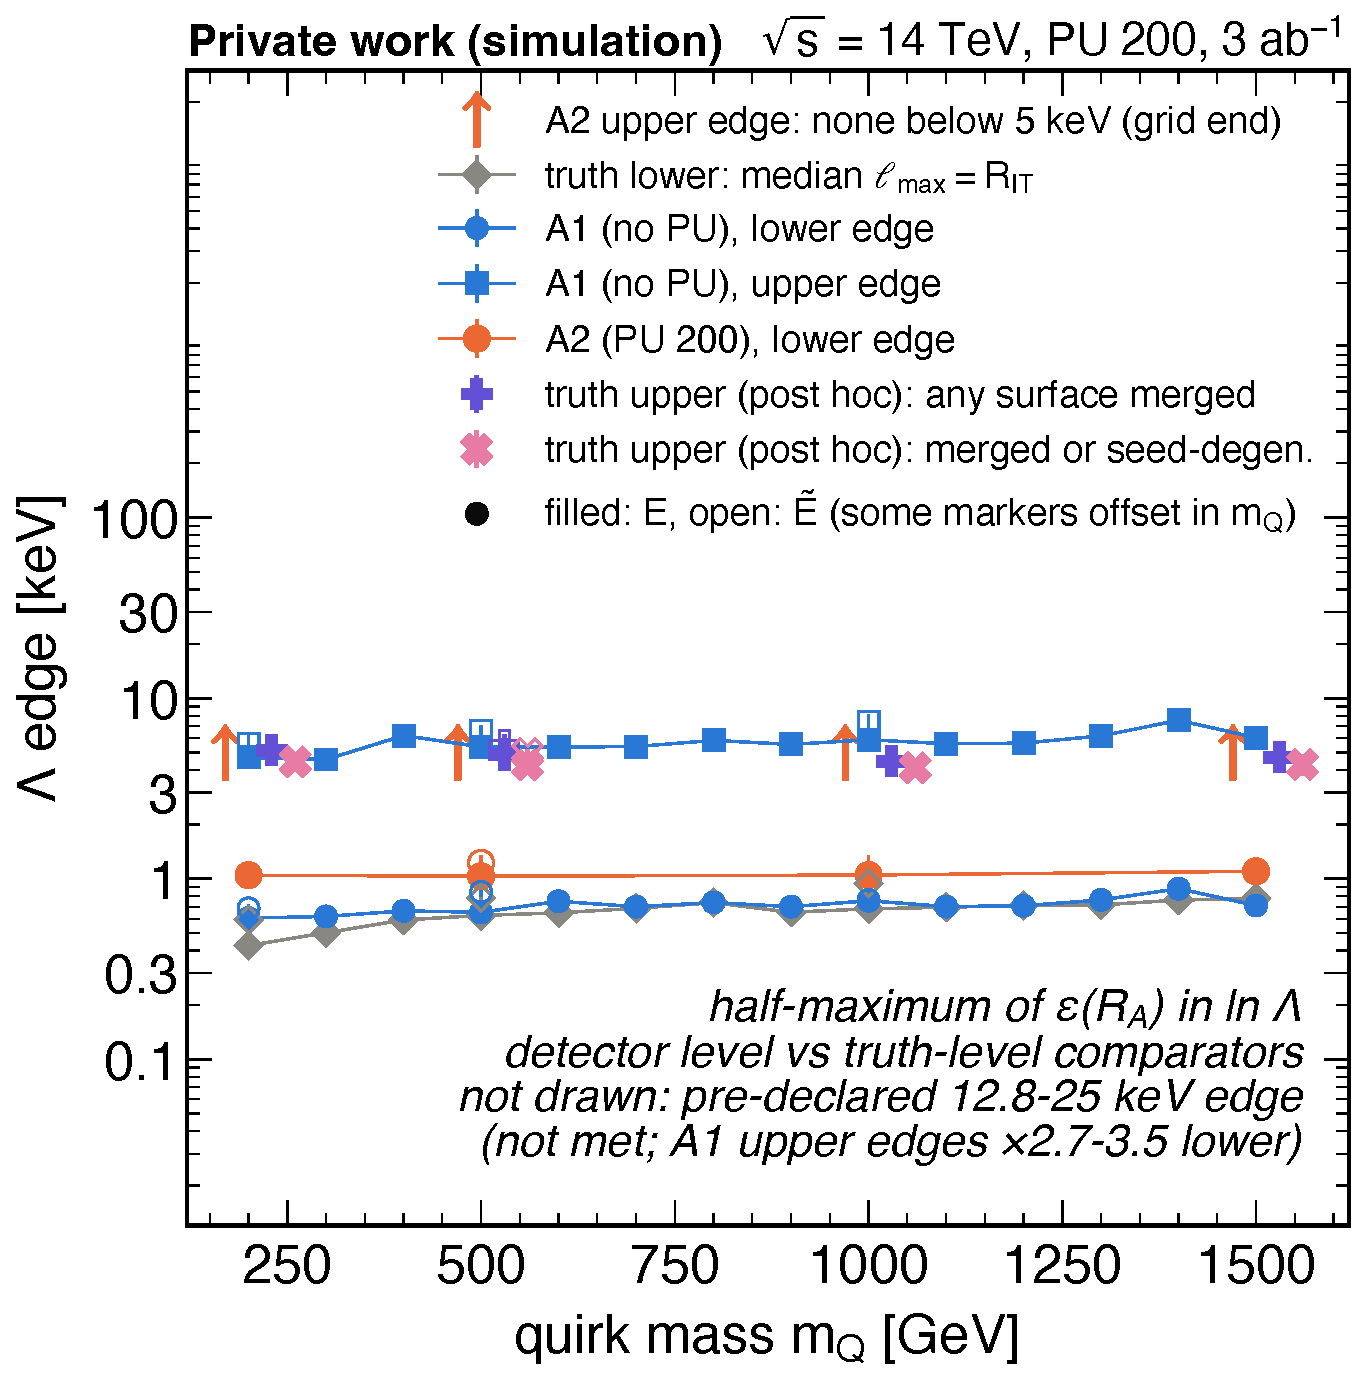
\includegraphics[height=0.37\linewidth]{figures/D9_edges_det_vs_truth.pdf}\hspace{0.02\linewidth}
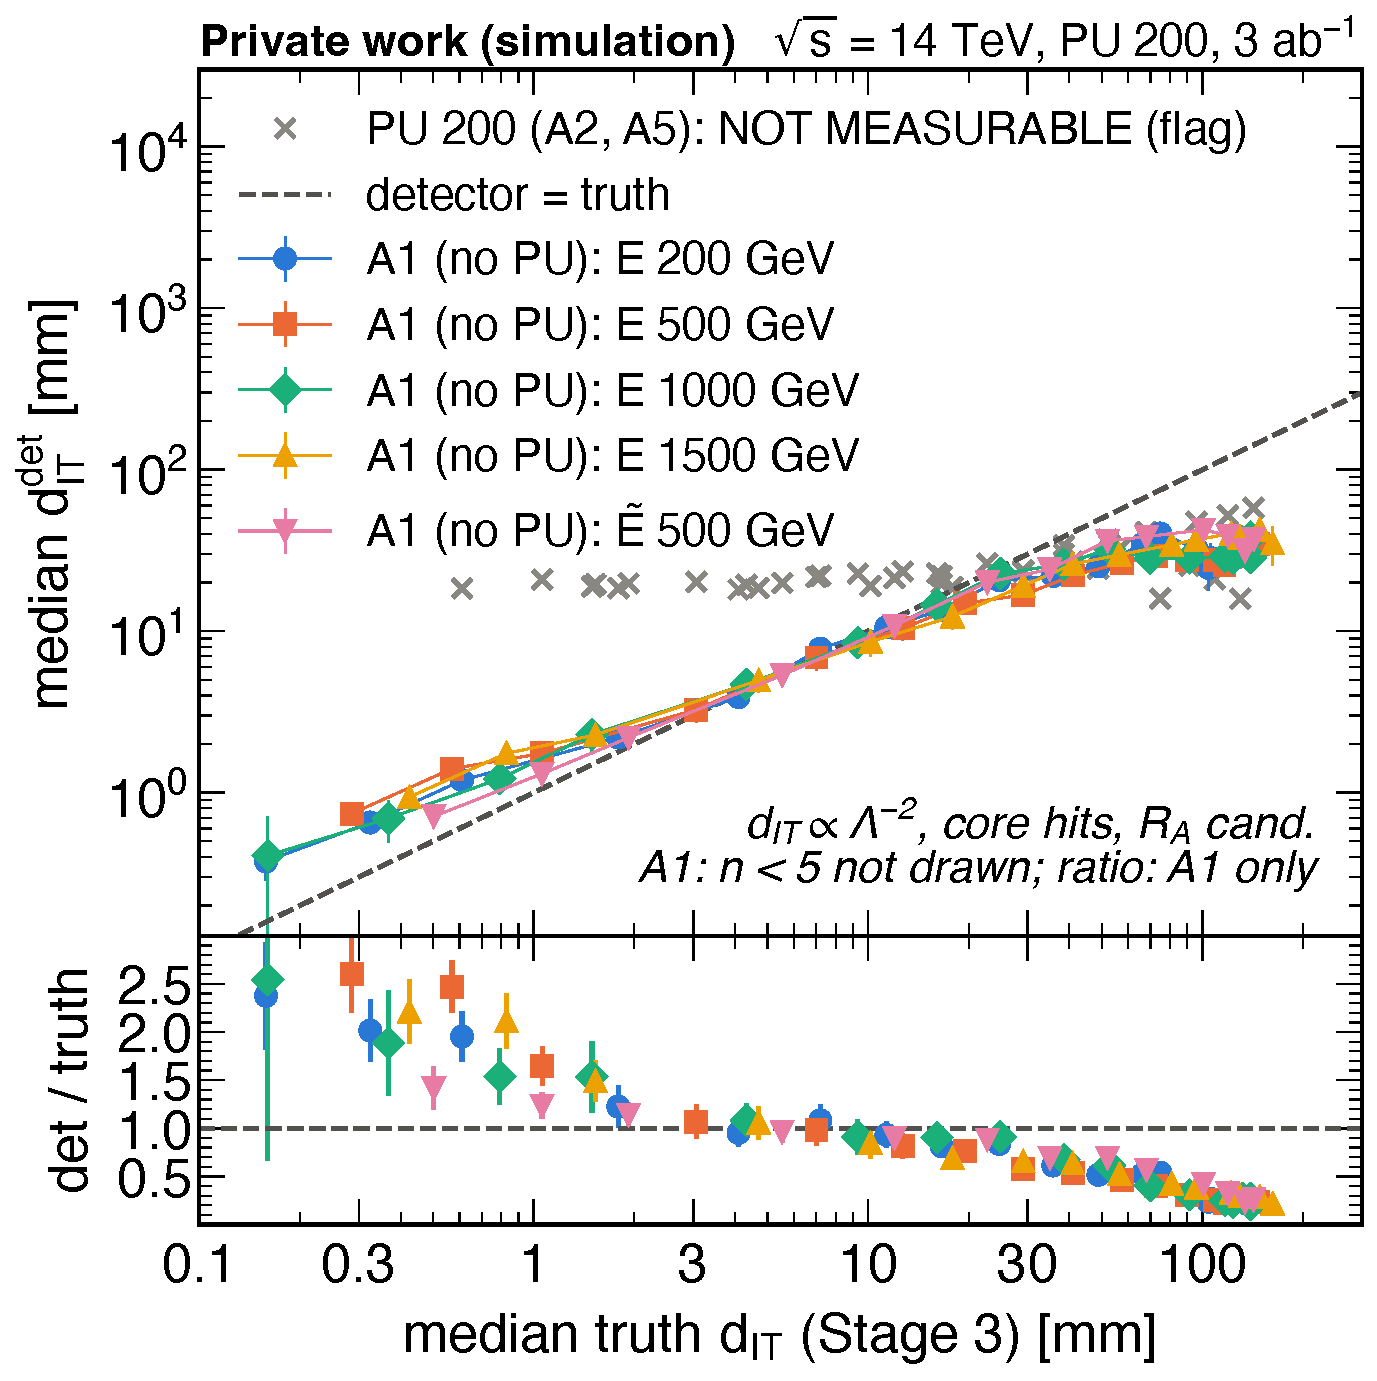
\includegraphics[height=0.37\linewidth]{figures/D10_sepit_calibration.pdf}
\caption{Detector-level $\Lam$ handles. (Left) Half-maximum edges of $\Eff$(R04) in $\ln\Lam$ against $\mQ$: lower and upper
edges without pile-up (A1), lower edges at PU 200 (A2; no upper edge below $5\keV$, arrows), and truth comparators (lower:
median $\lmax=\RIT$; upper, derived post hoc: 50\% of pairs with a merged surface, or merged or seed-degenerate). The
pre-declared 12.8--25\,keV comparator is not drawn and is not met. (Right) Median measured IT pair separation against the
truth: without pile-up (coloured) it tracks the truth at 3--20\,mm; at PU 200 (grey) it is flat and flagged not measurable.}
\label{fig:edgesdet}
\end{figure}

\subsection{Detector-level mass handles}\label{sec:mlam:mass}
The pre-declared mass estimator combines the MET with the pair velocity measured by time of flight to the barrel timing
layer, $M_{\rm est}=\mathrm{MET}\cosh\eta_{\rm axis}/(\beta\gamma)_{\rm ToF}$ (user decision). Since $\mathrm{MET}\cosh\eta$
approximates the pair momentum, $M_{\rm est}$ estimates the \textbf{pair mass $M_{Q\bar Q}\ge2\mQ$, not $\mQ$}.
Figure~\ref{fig:mest} shows its distribution at R04 for two masses.
\begin{itemize}
\item \textbf{Without pile-up} no event falls below $1.5\mQ$ (0 of 9551; minimum $1.69\mQ$), and the pooled median is
  $2.46\mQ$, just above the threshold $2\mQ$.
\item \textbf{At pile-up 200} the pooled median is $2.26\mQ$ (850 events with a defined $M_{\rm est}$), but 29\% of the
  events fall below $1.5\mQ$ and 19\% below $0.5\mQ$: a low cluster from in-time pile-up timing hits, which make
  $\beta_{\rm ToF}\to1$. $M_{\rm est}$ is undefined for 6--41\% of the candidates. The per-mass medians keep the mass
  ordering (483/1113/2070/3137\,GeV for $E$ 200/500/1000/1500), but the 16\% quantiles are 155--332\,GeV for every mass.
\item \textbf{$\beta_{\rm ToF}$ and $dE/dx$.} The median $\beta_{\rm ToF}$ rises from 0.23--0.53 without pile-up to 0.39--0.68
  with it; the truncated-mean $dE/dx$ is diluted from 1.8--7.1 to 1.5--2.7 MIP and keeps only a weak mass ordering.
\item \textbf{$\wcore$ as the $\lmax$ observable.} Without pile-up its median falls monotonically with $\Lam$ above
  $\approx0.85\keV$ ($E$ 500: 13.1/5.5/2.4/1.3\,mm at 1/2/3/5\,keV); at pile-up 200 it flattens to $\approx10$--12\,mm at
  $\ge3\keV$, because pile-up hits enter the core.
\end{itemize}
\textbf{P2 verdict on $\mQ$ and $\Lam$.} At pile-up 200 this set-up measures neither $\mQ$ nor $\Lam$: it provides an
ordering of the masses through the pair-mass proxy, and brackets $\Lam$ by the efficiency window. No mass fit or template
was run. A pile-up-robust separation estimator and a timing selection that rejects in-time pile-up hits would be needed to
recover the truth-level handles.

\begin{figure}[htbp]
\centering
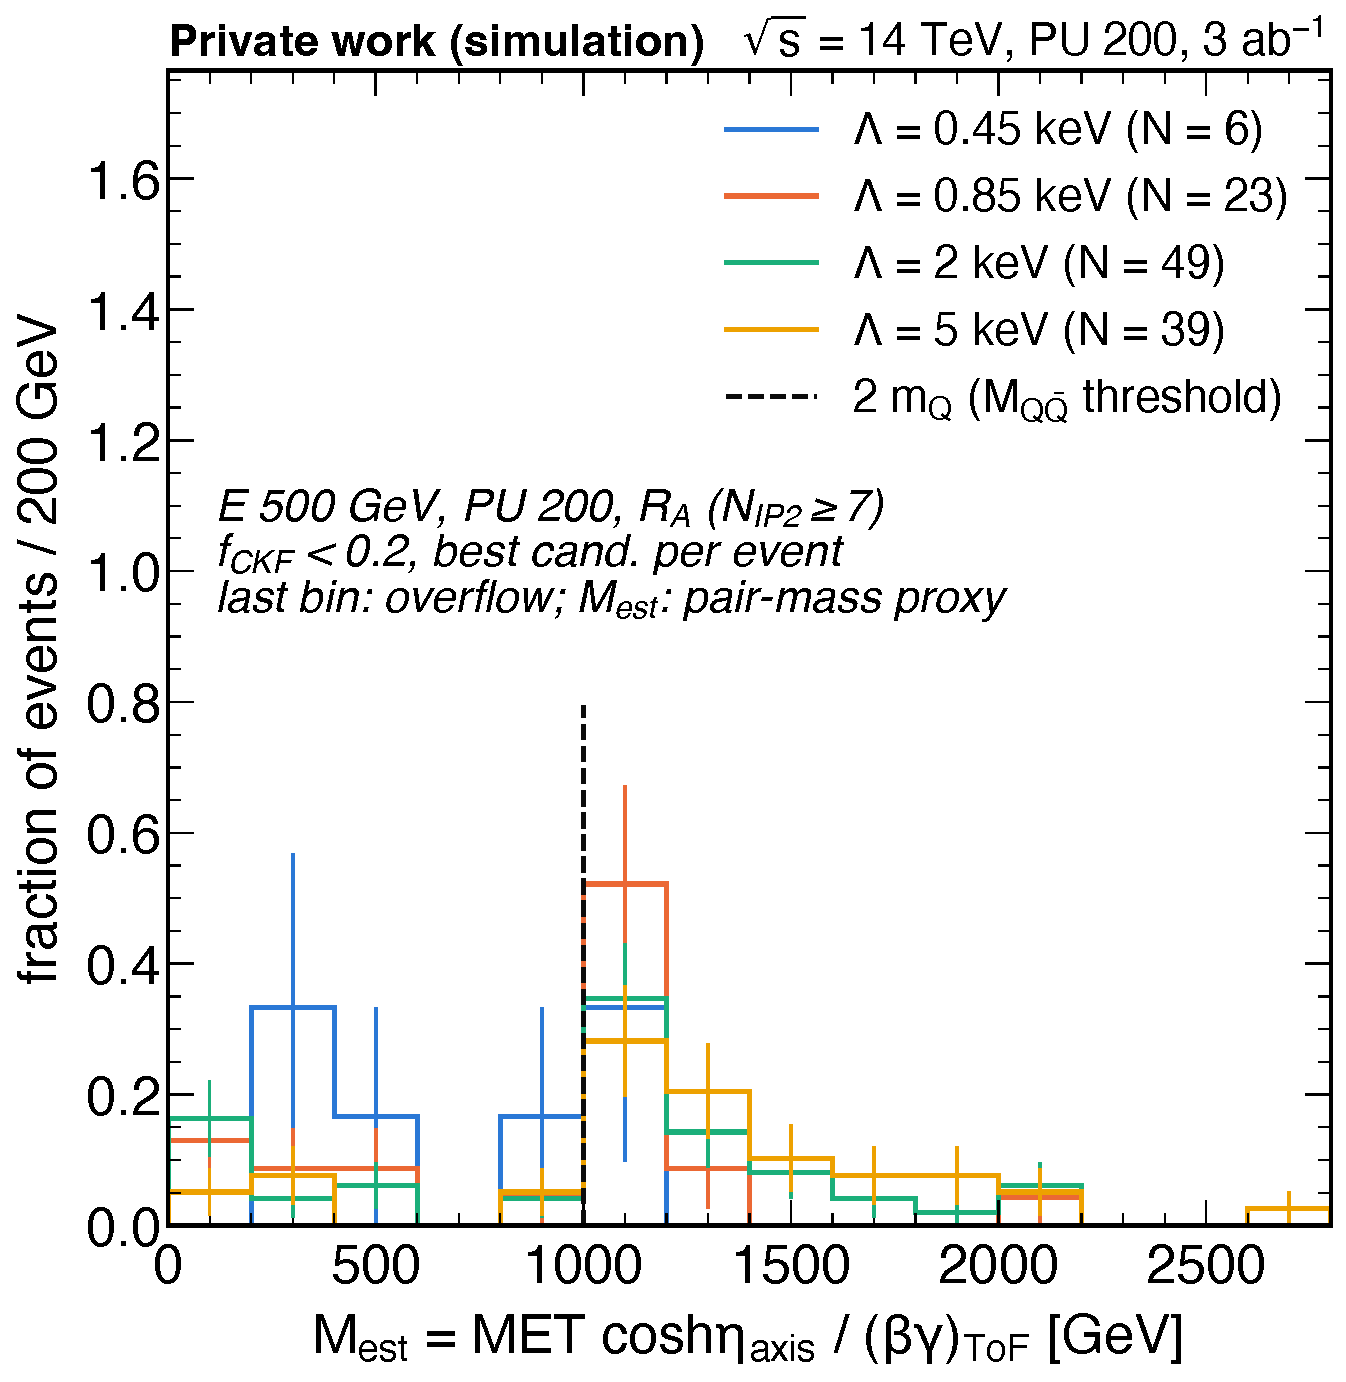
\includegraphics[height=0.38\linewidth]{figures/D8_mest_RA_F500.pdf}\hspace{0.02\linewidth}
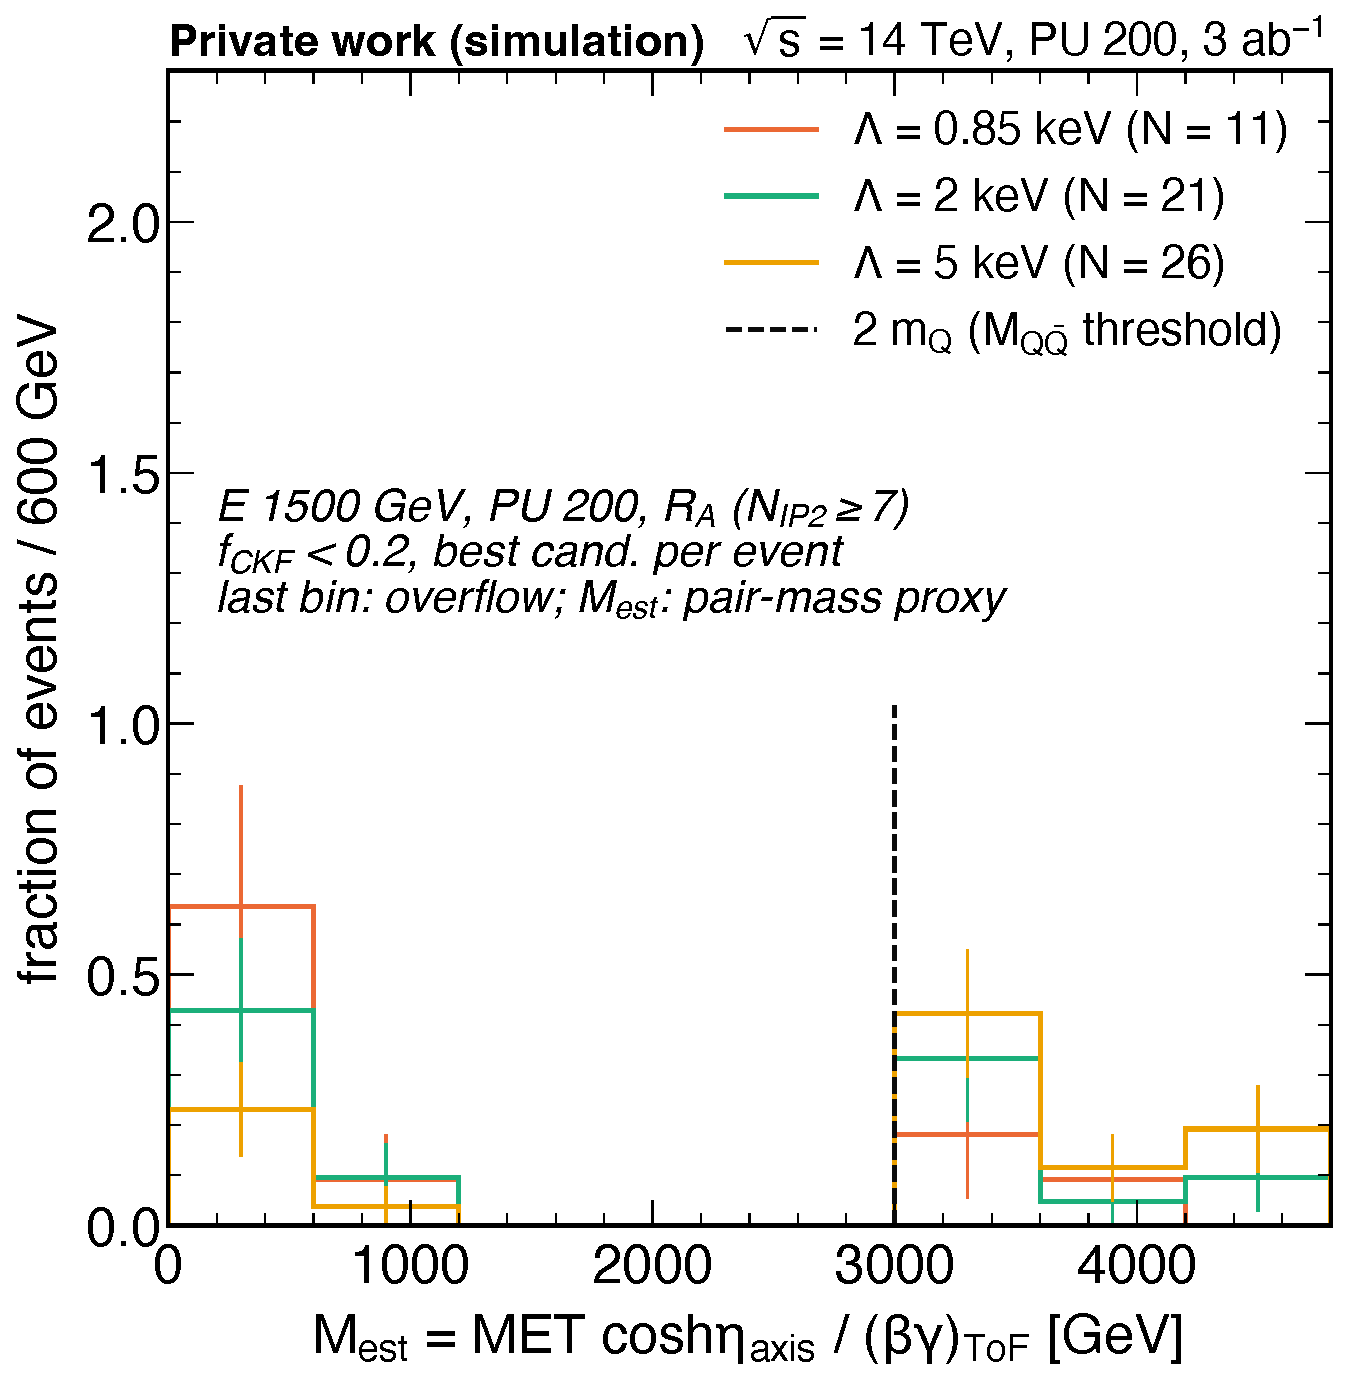
\includegraphics[height=0.38\linewidth]{figures/D8_mest_RA_F1500.pdf}
\caption{Distribution of the pair-mass proxy $M_{\rm est}=\mathrm{MET}\cosh\eta_{\rm axis}/(\beta\gamma)_{\rm ToF}$ at
detector level (PU 200, selection R04, best candidate per event, $f_{\rm CKF}<0.2$) for $E$ at 500 (left) and $1500\GeV$
(right), for several $\Lam$; the dashed line is $2\mQ$. The upper cluster starts near the pair-mass threshold $2\mQ$; the low
cluster at 0.1--0.4\,$\mQ$ comes from in-time pile-up timing hits. Nothing is expected near $\mQ$ itself. Per curve only
6--49 events enter, so the shapes are statistically weak.}
\label{fig:mest}
\end{figure}

\section{Comparison with existing bounds}\label{sec:bounds}

The expected sensitivity is compared with the published limits on the same benchmark. FASER's limits on the
$(1,1)_{-1}$ fermion with $N_{\rm IC}=2$~\cite{FASER:2026fsy,FASER:HEPData181308v1t2} are an exact model match and are
taken from HEPData; Farina and Low's recasts~\cite[Table~II]{Farina:2017cts} exclude $\mQ<650$ ($150$)$\GeV$ for $E$ and
$\mQ<350$ ($60$)$\GeV$ for $\Etil$ at $\Lam=1\eV$ ($100\eV$) and give no limit at $1\keV$; the D0 exclusion, $\mQ<107\GeV$ for
$\Lam=10\keV$--$1\MeV$~\cite{D0:2010kkd}, is a probable match (the SU(2)$_L$ representation is not stated). The
FASER-rendered heavy-stable-particle and monojet curves differ from Farina and Low's table at two points; the difference is
documented but not resolved (\rep{stage5/EXTERNAL_BOUNDS.md}).
In the $\Lam$ range of our grid ($0.45$--$5\keV$) all these bounds lie at $\mQ\lesssim180\GeV$, below the lightest
mass of the grid. Figure~\ref{fig:excl} shows the expected
$\sigma_{95}/\sigma_{\rm norm}$ of the fallback on the full $(\mQ,\Lam)$ grid of the fermion with the FASER exclusion
overlaid; the other limits fall outside the plotted range and are listed in the caption. No cell is below one (minimum 790 at $200\GeV$,
$1.5\keV$), so no exclusion, $\pm1\sigma$ or discovery contour exists. \textbf{This study therefore adds no exclusion beyond
the existing bounds}; it quantifies how far a barrel-only plane search at pile-up 200, with backgrounds estimated purely from
simulation, is from sensitivity.

\paragraph{Comparison with published reach projections.} Our null result comes from the background method, not from a
tension with Knapen et al.~\cite{Knapen:2017kly} and Li et al.~\cite{Li:2019wce}. With zero background our fallback
efficiencies would exclude $E$ up to $\approx1\TeV$ with $3\abinv$, and give a 5-event reach of $\approx0.6\TeV$ with
$300\fb^{-1}$, close to the $650\GeV$ of Knapen et al.\ (\EST{}, with $f_{200}$; their set-up differs: 2\,T field,
$\sqrt s=13\TeV$, eight-layer ATLAS-like barrel); our total efficiency
($f_{200}A\,\Eff\approx0.005$ at $E$ 500, barrel only) is about four times below theirs. An exclusion at $E$ 200,
$1.5\keV$ would need a total background below $\approx8\times10^2$ events ($\sigma_{\ln}=1$, \EST{}), whereas our estimate
there is a zero-count upper bound of $\sim6\times10^5$ events (median) from 500--2000 simulated events per process, set
by single-interaction topologies (PV pairs, decays in flight, nuclear interactions, loopers) that neither study treated
and by SM terms estimated here at the zero-count level, none of which scales with pile-up. Both studies assumed zero or a
small background after their cuts. We therefore do not
show those projections to be wrong: at pile-up 200 the background-free assumption cannot be confirmed by simulation alone.

\begin{figure}[htbp]
\centering
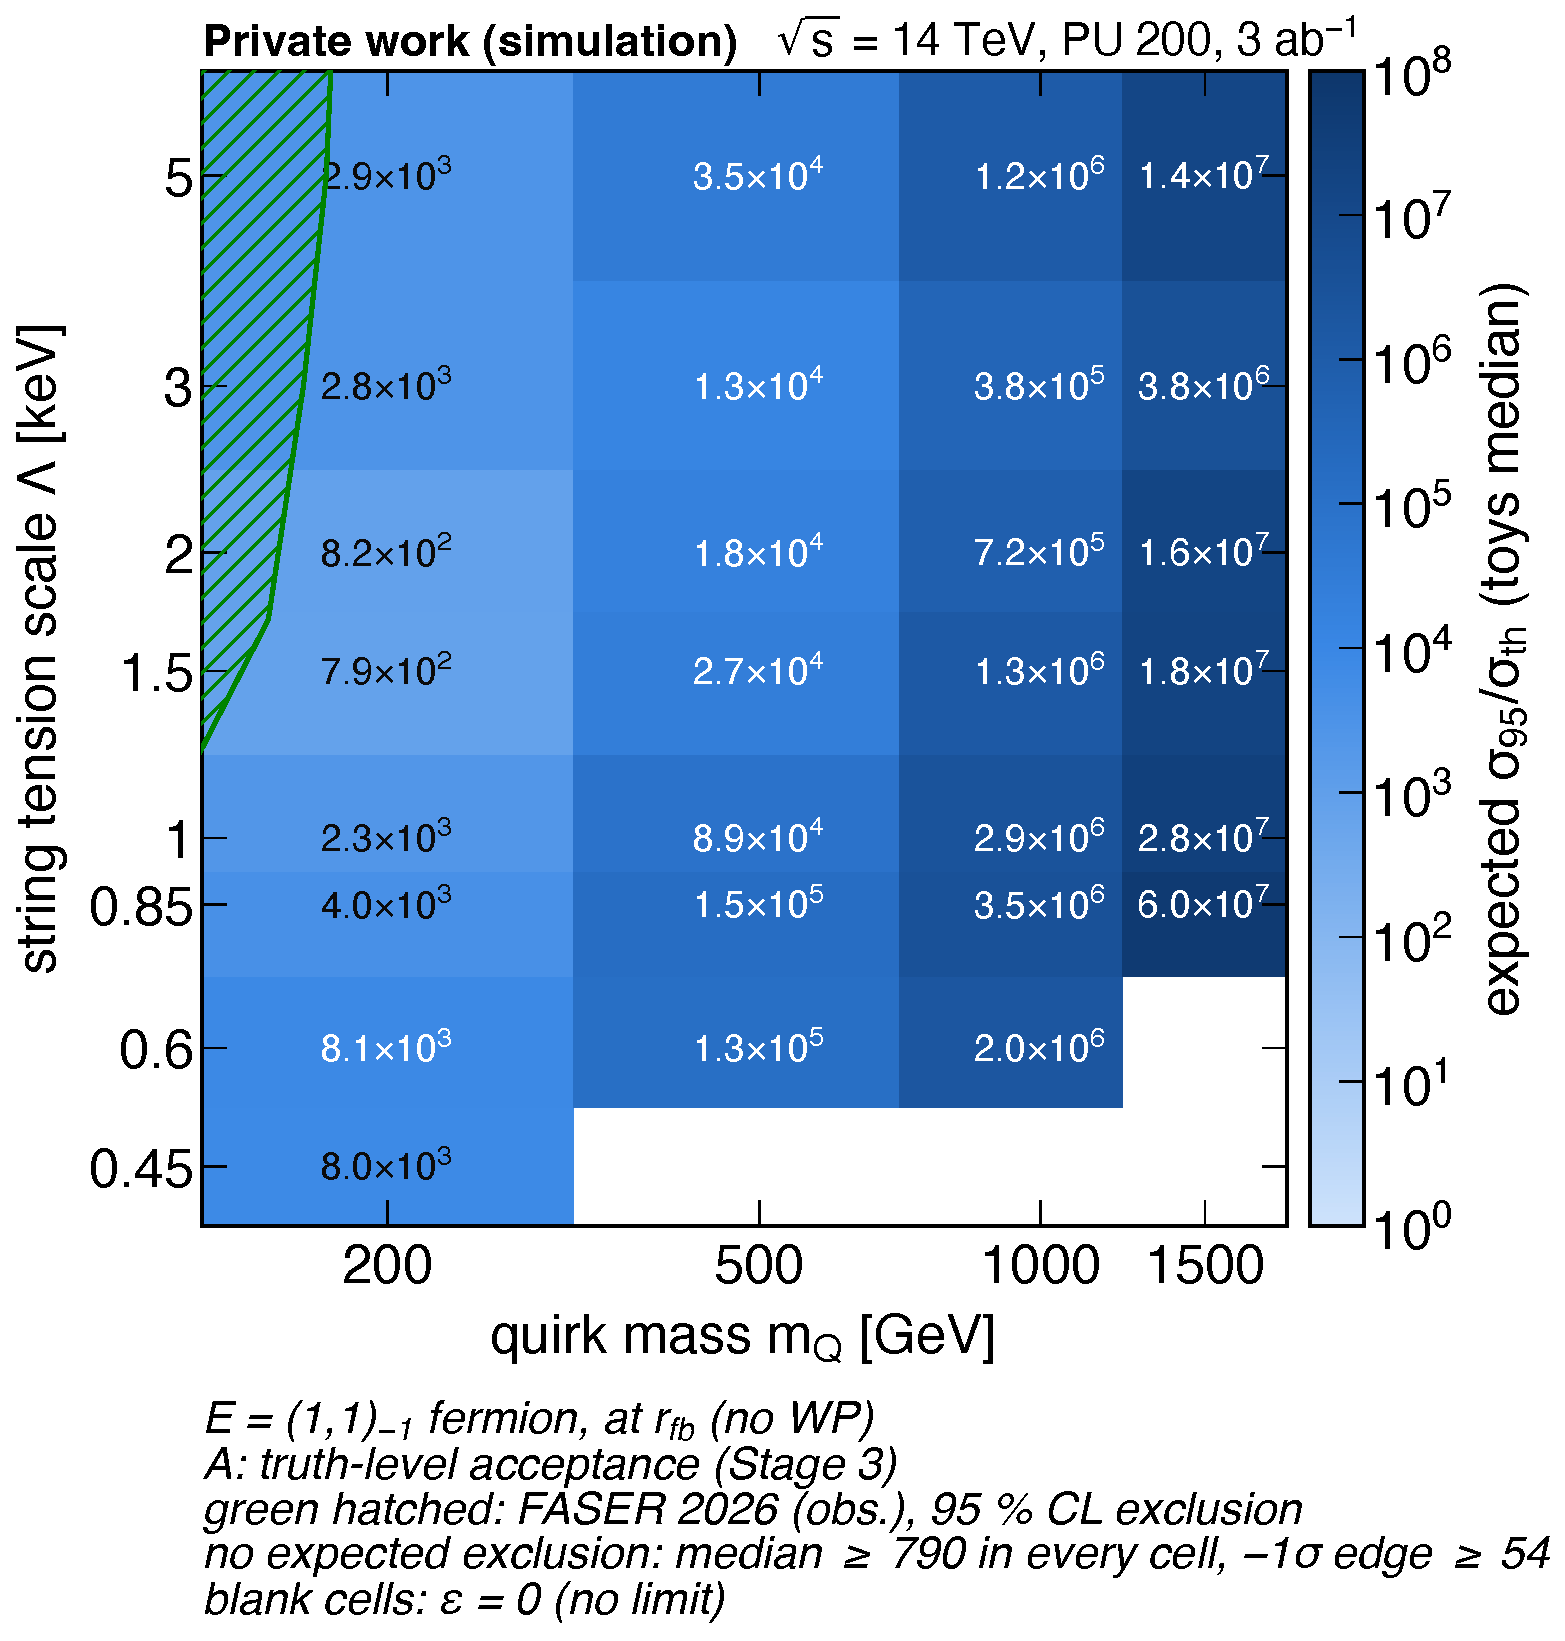
\includegraphics[height=0.44\linewidth]{figures/D7_exclusion_map.pdf}
\caption{Expected $\sigma_{95}/\sigma_{\rm norm}$ (toy median; labelled $\sigma_{95}/\sigma_{\rm th}$ in the figure) at the fallback selection on the
$(\mQ,\Lam)$ grid of the fermion $E$ (detector-level limit with truth-level acceptance; no working point). Every cell is
above one (median $\ge790$; the $-1\sigma$ toy edge $\ge54$), so nothing is excluded; blank cells have zero efficiency. The hatched region is the observed FASER exclusion~\cite{FASER:2026fsy}. Outside the plotted range lie
D0 ($\mQ<107\GeV$ at $\Lam=10\keV$--$1\MeV$~\cite{D0:2010kkd}), the Farina--Low benchmarks at $\Lam=1$ and
$100\eV$~\cite{Farina:2017cts}, and, as drawn by FASER, the heavy-stable-charged-particle recast
($\Lam\approx0.0024$--$0.22\keV$, $\mQ<685\GeV$), the monojet recast ($\mQ<57\GeV$) and the Evans--Luty out-of-time recast
($\Lam\approx0.0025$--$0.15\keV$, $\mQ<202\GeV$)~\cite{Evans:2018jmd}. The deep-rung background central values are zero-count
simulation bounds; the 31 fast-path points may overestimate $\Eff$ by up to $\approx1/0.87$
(Section~\ref{sec:results:eff}).}
\label{fig:excl}
\end{figure}

\section{Outlook: validating background inputs with CMS Open Data}\label{sec:opendata}

Several simulation-only inputs of the P2 background estimate could be checked against CMS Open Data. A feasibility
study (\rep{opendata/STAGE6_FEASIBILITY.md}; nothing analysed) identified three checks (efforts \EST{}). (1) The rates of
nuclear-interaction, $V^0$ and photon-conversion vertices against radius per interaction, from the secondary-vertex
collections kept in AOD (2012 MinimumBias, 2015D ZeroBias), which would test the generator-level rates of
Section~\ref{sec:bkg:cprime}; about 1--2 weeks. (2) The cluster density per layer, total and in time, from RAW data
re-reconstructed in a container (e.g.\ the 2017E ZeroBias RAW record~\cite{CMS:ZeroBias2017E}) together with the matching
pile-up simulation, which would test the density top-up of Section~\ref{sec:detector:pu} in the Phase-1 detector; about
3--5 weeks. (3) A rough bound on in-time cosmic muons from the 2012 NoBPTX datasets. None of these can test the
quirk-specific inputs (string dynamics, the $10^{-9}$-level combinatorial fake rate, the signal efficiency), no released
sample contains a validation signal, and none fits the project deadline: they are follow-up work.

\paragraph{Policy caveat.} The CMS data preservation, re-use and open access policy~\cite{CMS:OpenDataPolicy2018} governs
the released data, and the portal's guide for research use directs members of the CMS Collaboration to an internal
document on the use of open data by individual members. \textbf{Before any CMS Open Data is used for this study, the
author(s) must confirm the applicable CMS rules for members}, as well as the Open Data terms of use and citation
requirements; the CC0 licence of the portal datasets does not remove those rules. This note makes no claim about what
either policy allows. Any Open-Data comparison shown in the future must keep the labelling used here (no CMS name or
logo).

\section{Known limitations}\label{sec:limits}

This section lists the limitations that most affect the conclusions: what each is, whether it was addressed, its
quantitative impact where known, and what would fix it. The full registry is Appendix~\ref{app:limits}, and the complete
caveat list of the detector-level study is \rep{acts/stage4/STAGE4_RESULTS.md} \S8.

\paragraph{P1 (truth level).}
\begin{enumerate}
\item \textbf{The population $c$ and the region above $\approx5\keV$.} On the full simulation the population median of $c$
  lies $+2$--$3\%$ above the prediction at $1\keV$ (a failed pre-set gate, read as an estimator effect, \EST{}); the
  $3$--$5\keV$ excess is attributed to $\Bstar$ only by a $\Bstar$-off comparison (\EST{}); above $5\keV$ an unattributed
  $\pm5\%$ is carried. The decisive floor tests (under one CPU-hour each) were not run. No P2 impact, since multiple
  scattering dominates there.
\item \textbf{One failed prediction}: the straight-string/NG thickness ratio at $\gst=2$ (0.50 against $0.75\pm0.08$).
\item \textbf{Material and kinematics.} The per-layer material is \UNV{} ($\times0.5/\times2$; it sets the floor,
  $\DsMS\propto(x/X_0)^{0.36\ldots0.62}$); the signal is LO-merged (recoil tail $\pm11$--15\%), with transcribed $K$-factors.
\end{enumerate}

\paragraph{P2 (detector level).}
\begin{enumerate}[resume]
\item \textbf{Simulation-statistics limited background.} Beyond R07 every leading background term is a zero-count bound;
  $10^8$--$3\times10^9$ events per sample would be needed against 500--2000 (Section~\ref{sec:bkg:ladder}). The limits are
  therefore statements about this set-up, conservative with respect to simulation statistics (item 5 can bias them either
  way), not the physics reach of a real search.
\item \textbf{Untested factorisation and trend dominance.} Beyond the $\rho=2$ reach (R06) the background rests on
  conditionals measured on substitute populations; the factorisation closure test is degenerate (not informative), so the
  deep-rung background could be off in either direction by an unknown factor. The pre-registered conservative trend term
  (2--6.3) and model spread (4.76) dominate $\sigma_{\ln}$ from R11 on, and the closure factor $\times2.41$ is applied.
\item \textbf{Proxies and estimates in the background sum.} Eight SM processes ($W(e\nu)$, $W(\mu\nu)$, $t\bar t$ dileptonic, $t$-channel top, $tW$, $WW$, $WZ$, $ZZ$) enter through flagged proxies (15--45\% of the
  SM term); the 5\% veto inefficiency, $K_{t\bar t}=1.9$, the nuclear-interaction PV-line factor 0.22 and $\Ntrig$ as physics
  are \EST{}; $Z(\tau\tau)$, lost-lepton $Z(\ell\ell)$ and multijets are not included; Fatras has no hadronic interactions or
  decays in flight (toys replace them), out-of-time pile-up is replaced by the TDR density top-up, and the trigger, PV and
  MET models are parametrised (\UNV{}).
\item \textbf{Signal efficiency.} V4-3 is partial with a post-hoc match definition; the detector upper $\Lam$ edge misses
  its pre-declared comparator; deep-rung and fallback efficiencies have few passing events (e.g.\ 9/200 at the best point);
  31 of 40 points use the fast signal path, which may overestimate $\Eff$ by up to $\approx1/0.87$ (\EST{}); the independent
  finder cross-check (V4-5) was not run and the seed-threshold regression check (V4-4) is partial;
  $\Eff_{\rm tot}=f_{200}A\,\Eff_{\rm sel}$ assumes independence. The Stage-2 tail-rate uncertainty of $f_{200}$,
  $+12$--15\%/$-11$--13\% from varying the matrix-element $\alpha_s$ in MadGraph (\EST{}; \rep{sim/VALIDATION.md}), is not
  propagated into the limit ratios.
\item \textbf{Scope.} Barrel only ($|\eta(\hat n_3)|<1$; the barrel fraction without pile-up is 0.19--0.28); no endcap
  finder, no merged-pair regime, no detector-level P1 (the out-of-plane resolution, 23--30$\um$, equals the MS floor);
  efficiencies and limits at 40 of the 307 points of the admissibility grid. The campaigns C2-C (more SM statistics), C4$'$
  (rest of the grid with the full chain) and a $\rho=3$ pile-up sample were deferred (user decisions).
\item \textbf{Bookkeeping.} Three G3 pilot jobs were excluded (ACTS navigation assertion; they affect only the pilot
  verdict); 11 events in admitted jobs were replaced by deterministic re-seeding after the same assertion; one full-chain job
  was admitted despite three unmeasured pile-up hits out of 145\,007 (decision D13; negligible effect); a cosmetic bug in the
  frozen product code leaves the MET azimuth of the event-display fake undefined (no number uses it).
\end{enumerate}

\section{Conclusions}\label{sec:concl}

We studied colour-neutral electroweak quirks with $\Lam\sim0.5$--$10\keV$ in a CMS Phase-2-like tracker, at truth level for
the physics of the plane thickness (P1) and at detector level with pile-up 200 for a search and the measurement of $\mQ$
and $\Lam$ (P2). The study uses public information only and is not a CMS result.

\paragraph{P1 verdict (truth level).} The B-field thickness of the quirk plane is generated at the near-miss crossings of the
oscillating pair: the solenoid field, an electric field in the pair frame, makes the ends miss by $\bodd$ at every second
crossing, and the string's transverse pull integrates to $\ln(\lmax/\bodd)$, which rotates the oscillation axis. This gives
an analytic form of the per-period rotation that Li et al.\ determined numerically, and the law
$\DsB\propto\epsB[\ln(1/\epsB)+C]$ with local slope $c=1/[\ln(1/\epsB)+C]\simeq0.104$ at $1\keV$ and $500\GeV$, i.e.\
$\DsB\approx\Lam^{-1.8}B^{0.9}$, nearly independent of $\mQ$. The law is confirmed by blind numerics at $1\keV$ and holds per
event on $2.2\times10^5$ simulated events within $\lmax/\RIT\lesssim0.6$ and $\kB\lesssim4$; the population median of $c$
exceeds the prediction by $2$--$3\%$ (a failed pre-set gate, read as an estimator effect), a larger $\kB$-dependent excess at
$3$--$5\keV$ is attributed to the CM magnetic field as an estimate, and one prediction (the straight-string ratio at $\gst=2$)
fails. Multiple scattering sets a floor of 10--28$\um$ and dominates above $\Lcross\approx1.2$--$1.9\keV$, and the two add
below quadrature in the crossover. For a search, the field thickness matters below $\approx1.5\keV$; above it, the finder
tolerance is set by material.

\paragraph{P2 verdict (detector level).} With a dedicated barrel plane finder, a pile-up overlay normalised to the TDR
occupancies and a working-point rule frozen before any signal efficiency, \textbf{no working point exists}: the lowest
background is $\Nbkgeightyfour=1.23\times10^6$ events (R09), 7.05 decades above the budget, and the deep-rung background
consists of zero-count bounds. The pre-registered fallback gives expected limits at best 790 times the predicted signal
($E$ 200, $1.5\keV$; $\approx910$--950 with the full-chain efficiency systematic; ratios corrected for the
$p_T(Q\bar Q)>200\GeV$ tail fraction of the cross section, which an earlier version omitted), so \textbf{nothing is excluded}, and the
study adds nothing to the existing bounds (all below $\approx180\GeV$ in this $\Lam$ range). At pile-up 200 neither $\mQ$ nor
$\Lam$ is measured: the time-of-flight estimator is a pair-mass proxy with a pile-up-induced low cluster, and the
$\Lam^{-2}$ separation handle is not measurable. The negative result is dominated by simulation statistics and by the
pile-up extrapolation uncertainty, not by an observed background.

\paragraph{What would be needed.} None of the following can be applied to the frozen analysis; each needs a new
pre-registration. (i) A \emph{data-driven pile-up fake estimate} in control regions (MET-road or $\Delta\phi$ sidebands, or
out-of-time crossings) to replace the thinning extrapolation and its trend and closure uncertainties, the decisive item.
(ii) Deeper pile-up simulation ($\rho=3$, or a closure test with a real lever arm at R07--R09), worth about one decade.
(iii) Single-interaction conditionals from the high-statistics no-pile-up gun samples with their own closure test (about two
decades on those bounds) and time-tag credit for prompt SM and single-interaction terms in SR-T (up to four decades there).
(iv) A merging-tolerant counting rung or a line-topology category at $\Lam\gtrsim3\keV$, a lower seed-opening cut and an
endcap finder, to raise the $\approx0.3$ barrel ceiling of the efficiency. (v) A pile-up-robust separation estimator and
in-time-hit rejection for the time of flight, to recover the $\Lam$ and $\mQ$ handles. Even with (ii) and (iii) the estimate
leaves $\approx0$--2 (SR-T) and 4--5 (SR-G) decades (\EST{}, from the previous analysis run; order of magnitude
unchanged), so (i) is essential. Validating the background inputs with
CMS Open Data (Section~\ref{sec:opendata}) and an analytic multiple-scattering theory of the plane thickness are natural
follow-ups.


\bibliographystyle{unsrtnat_hep}
{\footnotesize\setlength{\bibsep}{1pt}\setlength{\columnsep}{1.5em}
\begin{multicols}{2}\raggedright
\bibliography{references}
\end{multicols}}

\appendix
\section{Notation}\label{app:notation}

One symbol is used per quantity throughout. Where the stage reports or the literature use a different symbol, it is
given in the last column. Times of flight are written in natural units (speed of light set to one); the symbol $c$ is reserved for the
local slope of the thickness law.

\begin{center}
\scriptsize
\begin{longtable}{l>{\raggedright\arraybackslash}p{0.50\linewidth}l}
\toprule
symbol & meaning & elsewhere\\
\midrule
\endhead
$\Lam$, $\sigma=\Lam^2$ & string scale and tension; $\sigma=50.68\GeV/\mathrm{cm}\,(\Lam/\keV)^2$ & Ref.~\cite{Asadi:2025btr}: $\Lam=T_c$\\
$\mQ$ & quirk mass & $m$ (Stage 1)\\
$N_{\rm IC}$ & number of infracolours (2) & $N_c$, $N$\\
$E$, $\Etil$ & fermion and scalar benchmark, $(1,1)_{-1}$ & F, S in file names\\
$B$, $\Bzero$ & lab magnetic field; $\Bzero=3.8112\tesla$ & \\
$\Estar$, $\Bstar$ & CM-frame electric and magnetic fields of the pair & \\
$\epsB$, $\epsp$ & $qB/\sigma$; $q|\Estar_\perp|/\sigma$ & $\varepsilon$, $\varepsilon_\perp$\\
$\kB$ & $|\Bstar_\perp|/|\Estar_\perp|$ & \\
$\gst$, $\bst$ & Lorentz factor and speed of one quirk in the pair CM frame & $\gamma^*$, $v$\\
$\lzero$, $\lmax$ & $\mQ/\sigma$; maximum separation $2(\gst-1)\lzero$ & \\
$\Nosc$ & number of oscillations within the tracker & \\
$\bodd$ & miss distance at odd crossings & $b$\\
$\rot$, $\Theta$, $N_{\rm odd}$ & axis rotation per CM period; accumulated rotation $\Theta=N_{\rm odd}\rot$; number of odd crossings & $\eta$ (Li et al., Stage 1)\\
$G(\gst)$, $K(\gst)$ & log coefficient and constant of $\rot$ & $A_o$ (numerics)\\
$C$, $c$ & constant and local log slope of the thickness law & \\
$\alpha$; $\theta^*$, $\phi^*$ & CM angle between $\Estar$ and $\hat n$; polar angle and azimuth of $\hat n$ about $\hat\beta_{\rm cm}$ (App.~\ref{app:derivation}) & \\
$f_N$ & out-of-plane share of the axis rotation, $|\hat e_\perp\cdot\hat N|$; $f_N\sin\alpha=|\hat E^*\cdot\hat N|$ & \\
$F$, $g$ & dimensionless prefactor of the thickness law; twist factor of the plane fit ($\simeq0.23$), Eq.~\eqref{eq:D:law} & \\
$R_m$ & matching radius of the non-relativistic calculation (App.~\ref{app:der:nr}) & \\
$\mathcal R(f)$ & response per unit field, $\DsB(fB)/[f\DsB(B)]$ & $R(f)$ (Stage 1)\\
$R$ & tracker radius (in Eq.~\eqref{eq:law}) & \\
$\Ds$ & plane thickness through the PV, Eq.~\eqref{eq:ds} & \\
$\DsB$, $\DsMS$, $\DsBM$ & field only; material only; both (truth level) & $\Delta s_{B+M}$\\
$\Lcross$ & $\Lam$ at which median $\DsB=$ median $\DsMS$ & \\
$\RIT$ & outer radius of the IT barrel ($\approx14.6\cm$) & \\
$\sepIT$ & separation of the two quirks in the IT & sep$_{\rm IT}$\\
$\eta$, $\eta_{\rm pair}$ & pseudorapidity; of the pair momentum & \\
$\hat n$, $\hat n_2$, $\hat n_3$ & plane normal; in-plane transverse direction; plane axis & $n$, $n_2$, $n_3$\\
$W_c$, $t_{\rm tol}$, $\sigma_{\rm tot}$ & finder window (75\,mm); thickness tolerance (30\,$\mu$m); collection width & \\
$\Tseed$ & seed threshold (layers with $\ge2$ crossings) & $T_{\rm seed}$\\
$N_{\rm IT2}$, $N_{\rm IP2}$, $N_{\rm 2S2}$ & IT, IT+PS, 2S barrel layers with $\ge2$ crossings & \\
$\wcore$, $\chicore$ & robust core width; core-hit $\chi^2$ & \\
$\dninetyfive$ & MET road half-width (0.15\,rad) & $\delta_{\rm road}$\\
$f_{\rm CKF}$ & fraction of band hits on CKF tracks & \\
$\rho$ & pile-up density in units of a normalised PU-200 event & \\
$n_{\rm int}$ & number of interactions contributing to a candidate & $k$ (plan)\\
$f_{200}$ & fraction of $\sigma_{\rm norm}$ with $p_T(Q\bar Q)>200\GeV$ and $|\eta_{\rm pair}|<4$ (the tail sample) & $f$, f\_tail\\
$A$, $A_{\rm incl}$ & truth-level acceptance $\Eff_{\rm fid}\Eff_{\rm trig}\Eff_{\rm presel|trig}\Eff_{\rm PV}$ of the tail sample; $f_{200}A$ & $A$, A\_incl\\
$\Eff_{\rm sel}$, $\Eff_{\rm tot}$ & detector-level selection efficiency ($\Eff$ from Section~\ref{sec:results} on); $f_{200}A\,\Eff_{\rm sel}$ & $\varepsilon$, $\varepsilon_{\rm finder}$\\
$\Ntrig$ & SM events after trigger and preselection in $3\abinv$ & $N_{\rm trig}$\\
$\kappa$ & signal category, T (SR-T, late BTL hit) or G (SR-G) & $c$ (WP\_RULE)\\
$K_{\rm QCD}$ & QCD $K$-factor of the signal cross section & $K$, $K_{\rm WG}$\\
$K_{\rm SM}$ & $K$-factor of the SM background cross sections & $K$\\
$L$ & integrated luminosity ($3\abinv$) & \\
$\Nbkg$, $\Nbkgeightyfour$ & expected background; its 84th percentile & $B$, $B_{84}$\\
$\sigma_{\ln}$ & log-normal width of a background term & \\
$\sigma_{\rm norm}$ & signal cross-section normalisation, Eq.~\eqref{eq:signorm} & \\
$N_{\rm exp}$, $S$ & predicted yield in the acceptance $\sigma_{\rm norm}f_{200}LA$; selected yield $N_{\rm exp}\Eff_{\rm sel}$ & \\
$\mu$, $\mu_{95}$ & signal yield in the acceptance; its expected 95\% CL upper limit & \\
$\sigma_{95}$ & limit on the inclusive cross section, $\mu_{95}/(Lf_{200}A)$ & \\
$\sigma_{\rm th}$ & figure label for $\sigma_{\rm norm}$ & \\
R01--R23 & cumulative ladder rungs (Table~\ref{tab:ladder}) & \\
R$_A$--R$_E$ & fixed reporting selections: R04, R04 + $\wcore<18.75\mm$, R04 + $\wcore<4.7\mm$, R14, R23 & \\
$h$, $o$ & F1 helix-test and arm-opening linearity variables & \\
FB$_k$ & non-width part of R14 with the single width cut $\wcore<W_c/2^k$ (FB0: none) & \\
$r_{\rm fb}$, $k_{\rm adm}$, $e_{\rm adm}$ & fallback selection; admissible width index; admissible $dE/dx$ threshold & \\
$\Lam_R(\mQ)$, $R_{\rm eff}$ & smoothed $\Lam$ with median $\lmax=\RIT$; expected truncated-mean $dE/dx$ of the quirk & \\
$M_{\rm est}$, $\beta_{\rm ToF}$ & pair-mass proxy $\mathrm{MET}\cosh\eta_{\rm axis}/(\beta\gamma)_{\rm ToF}$; time-of-flight velocity & \\
\bottomrule
\end{longtable}
\end{center}

\section{Reproduction: where each number comes from}\label{app:repro}

This note summarises six stage reports of the project; each carries the full detail, the review trail and the code. All
paths are relative to the project root \rep{theory_track/}; commands are run there with the project's pixi environment
(\cmd{pixi run python \ldots}) unless stated. Decisions are logged in \rep{LOG.md}. The figures used here are listed with
their sources and checksums in \rep{paper/FIGURE_MANIFEST.md}; the bibliography provenance is
\rep{paper/BIB_PROVENANCE.md}.

\begin{center}
\scriptsize
\begin{longtable}{>{\raggedright\arraybackslash}p{0.15\linewidth}>{\raggedright\arraybackslash}p{0.37\linewidth}>{\raggedright\arraybackslash}p{0.37\linewidth}}
\toprule
note section & stage report (status) & numbers and reproduction\\
\midrule
\endhead
Sec.~\ref{sec:model} & Stage 2: \rep{sim/VALIDATION.md}, \rep{sim/SAMPLES.md}, \rep{sim/DEFERRED.md} (PASS, review R2) &
  \rep{sim/results/xsec.json}; loader \rep{sim/scripts/mg_events.py}; headlines regenerated by
  \rep{sim/scripts/val_headlines.py}\\
Sec.~\ref{sec:string} & Stage 1: \rep{analytic/NEAR_MISS_IMPULSE.md} v5.1, \rep{analytic/numerics/NUMERICS.md},
  \rep{analytic/NOVELTY_AUDIT.md} (PASS, review R4) & checks \rep{analytic/checks/cNN_*.py} (outputs next to them);
  predictions \rep{analytic/predictions.json}; numerics \rep{analytic/numerics/results/*.json}\\
Sec.~\ref{sec:p1}, \ref{sec:mlam:truth} & Stage 3: \rep{sim/stage3/README.md}, \rep{VALIDATION.md},
  \rep{HANDOVER_STAGE4.md} (PASS, review R3) & \rep{sim/stage3/results/P1.json}, \rep{P2.json};
  \rep{sim/stage3/scripts/p1_results.py}, \rep{p2_results.py}, \rep{make_docs.py}; B+MS panel
  \rep{acts/stage4/u2_panel/make_u2_panel.py}\\
Sec.~\ref{sec:detector}, \ref{sec:strategy} & Stage 4 design: \rep{acts/stage4/plan.md} (PASS, review R9),
  \rep{WP_RULE.md} (frozen), \rep{WP_RULE_PC19.md} (PASS, R3), \rep{HASH_ADDENDUM.md}, G1/G1b/G3 reports &
  production runner \cmd{python -m acts.stage4.run\_stage4 run --campaign <C1a|C1b|C2B>}; \rep{run_a2fc.py}\\
Sec.~\ref{sec:bkg}--\ref{sec:mlam:mass} & Stage 4 results: \rep{acts/stage4/STAGE4_RESULTS.md}, \rep{data/acts_stage4/analysis/STAGE4_SUMMARY.json} (PASS, review R3) &
  \cmd{python -m acts.stage4.analysis.run\_all --campaigns C1a,C1b,C2B,A2FC}; \cmd{python3 -I} \rep{acts/stage4/results/make_stage4_summary.py}; \rep{selfcheck_stage4.py}\\
Figs.~\ref{fig:bkg}--\ref{fig:excl} & Stage 5: \rep{stage5/FIGURES_FINAL.md}, \rep{EXTERNAL_BOUNDS.md} (PASS, review R2) &
  \rep{stage5/make_figures.py} \cmd{--final --results} \rep{data/acts_stage4/analysis/C12FC_v1} \cmd{--truth}\\
Sec.~\ref{sec:opendata} & Stage 6: \rep{opendata/STAGE6_FEASIBILITY.md} (PASS, review R3) & text only\\
Fig.~\ref{fig:schematic} & conceptual diagram & \rep{paper/figures/src/make_schematic.py}\\
\bottomrule
\end{longtable}
\end{center}

\paragraph{Build of this note.} From \rep{paper/}: \cmd{xelatex quirks\_p1p2\_note; bibtex quirks\_p1p2\_note; xelatex
quirks\_p1p2\_note; xelatex quirks\_p1p2\_note}.

\section{Limitation and decision index}\label{app:limits}

Each entry is tagged [A] assumption, [L] limitation or [D] decision (with its log reference). 

\begin{center}
\scriptsize
\begin{longtable}{lp{0.80\linewidth}}
\toprule
tag & entry\\
\midrule
\endhead
{[A]} & Classical Nambu--Goto string with point ends, $J=0$ at production, no infracolour radiation (Sec.~\ref{sec:string}).\\
{[A]} & $K$-factors transcribed from the LHC SUSY working-group slepton tables, applied at 14\,TeV (Sec.~\ref{sec:model:xsec}).\\
{[A]} & Per-layer material slabs (\UNV{}), $\times0.5/\times2$ (Sec.~\ref{sec:p1:prop}).\\
{[A]} & Trigger turn-on, PV and MET resolution parametrised (Sec.~\ref{sec:detector:pvmet}, \ref{sec:strategy:trig}).\\
{[L]} & Thickness law not verified above $\approx5\keV$; floor tests not run (Sec.~\ref{sec:string:valid}).\\
{[L]} & $3$--$5\keV$ excess: size measured, $\Bstar$ attribution \EST{}; O-1 not done (Sec.~\ref{sec:p1:law}).\\
{[L]} & Failed prediction: straight-string/NG ratio at $\gst=2$ (Sec.~\ref{sec:string:valid}).\\
{[L]} & QED FSR off the quirks absent; one-sided $\lmax$ systematic $-1.1\pm0.8\%$ (Sec.~\ref{sec:model:syst}).\\
{[L]} & Fatras: no hadronic interactions, no decays in flight; out-of-time pile-up replaced by the TDR top-up (Sec.~\ref{sec:detector:pu}).\\
{[L]} & Barrel only; no endcap category, no merged regime, no detector-level P1 (Sec.~\ref{sec:strategy:finder}).\\
{[D]} & P1 scope (b): B-field crossing physics only, MS as measured floor (user, 2026-10-11).\\
{[D]} & U-1\ldots U-5 approved as recommended: excess published with \EST{} attribution; B+MS panel; merged-regime toys
      at $E$ 1000/1200 only; simplified surfaces; smearing without ACTS merging (user, 2026-10-13).\\
{[D]} & D4-15: pile-up topped up to the TDR occupancy (user, 2026-10-13).\\
{[D]} & D4-12: barrel-only selection $|\eta(\hat n_3)|<1.0$ (user, 2026-10-13).\\
{[D]} & D4-17: fallback deliverable approved before production (user, 2026-10-13).\\
{[D]} & $\Tseed:=4$ (pre-declared G3 action) and conservative closure end state (user, 2026-10-14).\\
{[D]} & PC-19 SR-T window (user-approved design points, 2026-10-14).\\
{[D]} & D1: $\Ntrig$ counted after the event-level preselection (user, 2026-10-14).\\
{[D]} & A2FC full-chain revert of nine points (pre-registered rule) and admission of one job with a pile-up-only V4-1
      failure (D13, 2026-10-16).\\
{[L]} & No working point; deep-rung background = zero-count bounds; $10^8$--$3\times10^9$ events per sample needed (Sec.~\ref{sec:bkg:ladder}).\\
{[L]} & Factorisation beyond R06 without informative closure test; trend and model terms dominate $\sigma_{\ln}$; closure $\times2.41$ (Sec.~\ref{sec:bkg:closure}).\\
{[A]} & Flagged SM proxies, veto inefficiency 5\%, $K_{t\bar t}=1.9$, PV-line factor 0.22 (\EST{}) (Sec.~\ref{sec:bkg:sm}, \ref{sec:bkg:cprime}).\\
{[L]} & V4-3 partial (post-hoc match); upper $\Lam$ edge misses the pre-declared comparator; V4-5 not run (Sec.~\ref{sec:results:eff}, \ref{sec:mlam:det}).\\
{[L]} & Fast signal path at 31 of 40 points may overestimate $\Eff$ by up to $\approx1/0.87$ (\EST{}, not applied) (Sec.~\ref{sec:results:eff}).\\
{[L]} & $\sepIT$ not measurable at PU 200; $M_{\rm est}$ is a pair-mass proxy with a pile-up low cluster (Sec.~\ref{sec:mlam:det}, \ref{sec:mlam:mass}).\\
{[D]} & C2-C, C4$'$, $\rho=3$ (C5) and the endcap finder deferred to future work (user, 2026-10-13/14).\\
\bottomrule
\end{longtable}
\end{center}


\section{The near-miss mechanism step by step (full derivation of Section~\ref{sec:string})}\label{app:derivation}

Section~\ref{sec:string} gives the results of the P1 theory in condensed form. This appendix gives every step, in the
order in which the argument is built, so that it can be checked line by line. It follows the Stage-1 note
\rep{analytic/NEAR_MISS_IMPULSE.md} (v5.1); each step names the sympy or numerical check that verifies it
(\rep{analytic/checks/cNN_*.py}, with outputs next to them). Units are $\hbar=c=1$; the notation is that of
Appendix~\ref{app:notation}. Table~\ref{tab:derivation_status} at the end lists which steps are derived, which are
verified numerically and which are numerical only.

\subsection{Equations of motion}\label{app:der:eom}
The system is a classical Nambu--Goto (NG) string of tension $\sigma$ whose two ends carry point masses $\mQ$~\cite{Kang:2008ea}. Here the ends also carry
charges $q_1=+q$, $q_2=-q$ and sit in a uniform constant external field:
\begin{equation}
  S=-\sigma\int d^2\xi\,\sqrt{-\det h_{ab}}\;-\;\sum_{i=1,2}\mQ\int d\tau_i\;+\;\sum_{i=1,2}q_i\int A_\mu\,dx_i^\mu ,
  \label{eq:D:action}
\end{equation}
where $h_{ab}$ is the induced metric on the world sheet and $\tau_i$ the proper time of end $i$. Two consequences are
used throughout.
\begin{enumerate}
\item \textbf{The string is neutral.} The field acts only on the ends. The string exchanges momentum and angular momentum
  with the ends but conserves the totals, so the total momentum and the total angular momentum (ends plus string) change
  only through the Lorentz forces on the ends.
\item \textbf{Bulk and boundary.} For a string lying along $x$ with a small transverse displacement $y(t,x)$, the static
  gauge $X^\mu=(t,x,y(t,x))$ gives the Lagrangian density $-\sigma\sqrt{1+y_x^2-y_t^2}\simeq-\sigma+\tfrac{\sigma}{2}(y_t^2-y_x^2)$.
  So $y$ obeys the wave equation $y_{tt}=y_{xx}$ and the string carries the transverse momentum density $\sigma y_t$.
  The force that the string exerts on an end follows from momentum balance (Section~\ref{app:der:wedge}). For a straight
  string whose end moves along it, the force is $-\sigma\hat s$, of magnitude $\sigma$ and directed toward the other end.
\end{enumerate}
The infracolour gauge group enters only through $\sigma=\Lam^2$. All results below therefore hold for any $N_{\rm IC}$
and representation once $\sigma$ is fixed.

\subsection{From the lab solenoid to the pair rest frame}\label{app:der:frame}
In the lab there is only a magnetic field $\mathbf B=B\hat z$. Let $\boldsymbol\beta_{\rm cm}$ be the initial velocity of
the pair and $\gamma_{\rm cm}$ its Lorentz factor. The standard field transformation (e.g.\ Jackson, Sec.~11.10) gives,
in the frame moving with $\boldsymbol\beta_{\rm cm}$ (``CM frame''),
\begin{equation}
  \Estar=\gamma_{\rm cm}\,\boldsymbol\beta_{\rm cm}\times\mathbf B,\qquad
  \Bstar=\gamma_{\rm cm}\mathbf B-(\gamma_{\rm cm}-1)(\mathbf B\cdot\hat\beta_{\rm cm})\,\hat\beta_{\rm cm}.
  \label{eq:D:fields}
\end{equation}
Both fields are uniform and constant, and $|\Estar|=\gamma_{\rm cm}\beta_T B$, with $\beta_T$ the component of
$\boldsymbol\beta_{\rm cm}$ transverse to $\hat z$. The action~\eqref{eq:D:action} is Lorentz invariant. One can therefore
solve the problem in the CM frame and boost the hits back to the lab, and no simultaneity convention enters. In the CM
frame the two ends start at the origin with momenta $\pm p^*\hat n$. Here $\hat n$ is the direction of end~1 (charge $+q$)
and $p^*=\mQ\rho$ with $\rho\equiv\gst\bst$. The pair invariant mass is $M=2\mQ\gst$, so
\begin{equation}
  \gamma_{\rm cm}\beta_T=\frac{p_T}{M}=\frac{p_T}{2\mQ\gst}.
  \label{eq:D:gbT}
\end{equation}
Split $\Estar$ into its components along $\hat n$ and perpendicular to it, $\Estar_\perp=|\Estar_\perp|\hat e_\perp$,
and let $\alpha$ be the angle between $\Estar$ and $\hat n$. The dimensionless field strengths of Eq.~\eqref{eq:eps} are
then
\begin{equation}
  \epsB=\frac{qB}{\sigma},\qquad
  \epsp=\frac{q|\Estar_\perp|}{\sigma}=\epsB\,\gamma_{\rm cm}\beta_T\sin\alpha,\qquad
  \kB=\frac{|\Bstar_\perp|}{|\Estar_\perp|}.
  \label{eq:D:eps}
\end{equation}
With $qB=2.998\times10^{-3}\GeV/\mathrm{cm}$ per tesla and $\sigma=50.68\GeV/\mathrm{cm}\,(\Lam/\keV)^2$, one gets
$\epsB=2.254\times10^{-4}$ at $3.8112\tesla$ and $1\keV$. Typical events have $\epsp\sim10^{-5}$--$10^{-4}$ at $1\keV$,
so the field is a very weak perturbation of the string force.

\subsection{The vacuum yo-yo (zeroth order)}\label{app:der:yoyo}
\paragraph{Solution.} Without fields the string stays straight along $\hat n$ and each end moves along it. The force on
each end is therefore exactly $\sigma$, directed toward the other end~\cite[Sec.~3]{Kang:2008ea}. For end~1,
$dp_1/dt=-\sigma$, so $p_1(t)=p^*-\sigma t$ and
\begin{equation}
  x_1(t)=\int_0^t\frac{p_1\,dt'}{\sqrt{\mQ^2+p_1^2}}=\frac{1}{\sigma}\Bigl[\sqrt{\mQ^2+p^{*2}}-\sqrt{\mQ^2+(p^*-\sigma t)^2}\Bigr].
\end{equation}
The separation $x=x_1-x_2=2x_1$ is therefore~\cite{Kang:2008ea} (check \rep{c01} (1))
\begin{equation}
  x(t)=2\lzero\Bigl[\gst-\sqrt{1+(\rho-t/\lzero)^2}\Bigr],\qquad 0\le t\le T_h=\frac{2p^*}{\sigma}=2\rho\lzero,
  \qquad \lzero=\frac{\mQ}{\sigma}.
  \label{eq:D:x}
\end{equation}
It vanishes at $t=0$ and $t=T_h$, reaches $\lmax=2(\gst-1)\lzero$ at $t=\rho\lzero$, and the ends pass each other at
speed $\bst$. At $t=T_h$ the ends pass \emph{through} each other, and the next half-period is the mirror image,
$x(t+T_h)=-x(t)$. The full CM period is $2T_h=4p^*/\sigma$. We number the crossings $j=1,2,\ldots$: odd $j$ at
$t=T_h,3T_h,\ldots$, even $j$ at $t=2T_h,4T_h,\ldots$ (production is the crossing $j=0$).

\paragraph{Zero-length string at the crossings.} The world sheet is a chain of flat ``lenses'' bounded by the two end
world lines, which touch at the crossings. At a crossing the string has zero length, and hence zero energy, momentum and
angular momentum. The whole state is given by the two end momenta at a common point.

\paragraph{Half-period integral.} The torque in Section~\ref{app:der:torque} needs $I\equiv\int_0^{T_h}x\,dt$.
Substitute $u=\rho-t/\lzero$ and use $\sqrt{1+\rho^2}=\gst$ (check \rep{c01} (2)):
\begin{equation}
  I=2\lzero^2\int_{-\rho}^{\rho}\bigl[\gst-\sqrt{1+u^2}\bigr]du
   =2\lzero^2\Bigl[2\rho\gst-\bigl(\rho\sqrt{1+\rho^2}+\operatorname{asinh}\rho\bigr)\Bigr]
   =2\lzero^2\bigl[\gst\rho-\operatorname{asinh}\rho\bigr].
  \label{eq:D:I}
\end{equation}

\paragraph{Rigid-rotation lemma.} \emph{A transverse momentum $\Delta p_\perp$ given to the relative motion around a crossing
rotates the whole later motion rigidly by $\delta=\Delta p_\perp/p^*$.} Proof: at a crossing the string has zero length
(previous paragraph), so the state is two point momenta at one point. Without fields the equations are rotation
invariant, so the rotated initial state evolves into the rotated vacuum solution. A kick changes the momenta from
$\pm p^*\hat n$ to $\pm(p^*\hat n+\Delta p_\perp\hat e)$, which equals $\pm p^*(\hat n+\delta\hat e)$ up to a change of
magnitude of $O(\delta^2)$. The subsequent motion is the yo-yo along the axis $\hat n+\delta\hat e$. In other words, the
axis direction is a zero mode of the yo-yo. Anything that happens in a short window around a crossing acts on the
long-time motion only through this zero mode.

\subsection{Torque, angular momentum and the miss distance}\label{app:der:torque}
\paragraph{Torque law.} Let $\mathbf J=\sum_i\mathbf x_i\times\mathbf p_i+\mathbf J_{\rm string}$ be the total angular
momentum about the CM. By item~1 of Section~\ref{app:der:eom} it changes only through the Lorentz forces on the ends:
\begin{equation}
  \frac{d\mathbf J}{dt}=\sum_i\mathbf x_i\times q_i\bigl(\Estar+\mathbf v_i\times\Bstar\bigr).
\end{equation}
To first order in the field, evaluate the right-hand side on the yo-yo, where $\mathbf x_2=-\mathbf x_1$,
$\mathbf v_2=-\mathbf v_1$ and $q_2=-q_1$. The magnetic terms cancel exactly:
$\mathbf x_1\times q(\mathbf v_1\times\Bstar)+(-\mathbf x_1)\times(-q)\bigl((-\mathbf v_1)\times\Bstar\bigr)=0$. Their
contribution to the relative force, $(\mathbf F_1-\mathbf F_2)/2$, also vanishes (check \rep{c01} (4)). The electric term
gives
\begin{equation}
  \frac{d\mathbf J}{dt}=q(\mathbf x_1-\mathbf x_2)\times\Estar=q\,x(t)\,\hat n\times\Estar
  =q|\Estar_\perp|\,x(t)\,\hat n\times\hat e_\perp .
  \label{eq:D:torque}
\end{equation}
Only $\Estar_\perp$ produces a torque, and in linear response $\Bstar$ does nothing to the relative motion. The
symmetry reason is that under inversion through the CM combined with exchange of the ends, the $\Estar$ force is even
and the $\Bstar$ force is odd.

\paragraph{The alternating pattern.} Integrating Eq.~\eqref{eq:D:torque} over the first half-period gives
$\mathbf J(T_h)=q|\Estar_\perp|\,I\,\hat n\times\hat e_\perp$. Over the second half-period $x$ changes sign, so
$\mathbf J(2T_h)=0$. The angular momentum is therefore zero at production and at every even crossing, and equal to
$\mathbf J_{\rm odd}=q|\Estar_\perp|I\,\hat n\times\hat e_\perp$ at every odd crossing (Li et al.'s ``meet at
$g=2n$''~\cite[Eqs.~(A.4)--(A.5)]{Li:2020aoq}, here with the value at the odd crossings).

\paragraph{Miss distance.} At an odd crossing the string has zero length, so $\mathbf J$ is carried by the ends. If they
pass at transverse offsets $\pm(b/2)\hat s$ with momenta $\mp p^*\hat n$ (end~1 is now moving back),
$\mathbf J=\tfrac b2\hat s\times(-p^*\hat n)+(-\tfrac b2\hat s)\times(p^*\hat n)=b\,p^*\,\hat n\times\hat s$. Comparing
with $\mathbf J_{\rm odd}$ gives $\hat s=\hat e_\perp$: the positive end passes on the $+\Estar_\perp$ side, as
expected. The miss distance is $b=J/p^*$. With Eq.~\eqref{eq:D:I}, $p^*=\mQ\rho$ and $\lzero^2/\mQ=\lzero/\sigma$
(check \rep{c01} (3)):
\begin{equation}
  \bodd=\frac{q|\Estar_\perp|\,2\lzero^2(\gst\rho-\operatorname{asinh}\rho)}{\mQ\rho}
  =2\epsp\lzero\Bigl[\gst-\frac{\operatorname{asinh}\rho}{\rho}\Bigr],\qquad
  \frac{\bodd}{\epsp\lmax}=\frac{\gst-\operatorname{asinh}\rho/\rho}{\gst-1}.
  \label{eq:D:bodd}
\end{equation}
This is Eq.~\eqref{eq:bodd}. For slow ends, $\gst\simeq1+\rho^2/2$ and $\operatorname{asinh}\rho/\rho\simeq1-\rho^2/6$,
so $\gst-\operatorname{asinh}\rho/\rho\simeq\tfrac23\rho^2$ and $\bodd\to\tfrac43\epsp\lzero{\bst}^2$, i.e.\
$\bodd/(\epsp\lmax)\to4/3$. The ratio is 1.327/1.298/1.240/1.188 at $\gst=1.05/1.3/2/3$. The causal solver reproduces it to $10^{-4}$
(check \rep{c03}); two solvers (causal and conformal) agree with it to $\le10^{-3}$ (Table~\ref{tab:numerics}). Even crossings have $b=0$ at this order. At $500\GeV$, $1\keV$ a
typical event has $\epsp\approx5\times10^{-5}$ and $\lmax\approx4.5\cm$, so $\bodd\approx3\um$, against a median of
$\approx3.5\um\,(\keV/\Lam)^4$ over the sample (the $\Lam^{-4}$ comes from $\epsp\propto\Lam^{-2}$ and $\lzero\propto\Lam^{-2}$).

\subsection{Linear response and where it fails}\label{app:der:linear}
The failure is easiest to see for a straight string with slow ends. Let $\mathbf r=\mathbf x_1-\mathbf x_2=x\hat
n+z\hat e_\perp$, with reduced mass $\mu=\mQ/2$. Each end is pulled toward the other with force $\sigma$, so
$\mu\ddot{\mathbf r}=-\sigma\hat{\mathbf r}+q\Estar$. Its transverse component, to first order in $z$, is
\begin{equation}
  \mu\ddot z=-\sigma\frac{z}{|x(t)|}+q|\Estar_\perp| .
  \label{eq:D:zlin}
\end{equation}
Three exact properties follow (the third is used in check \rep{c05}).
\begin{enumerate}
\item $z=\theta_0x(t)$ solves the homogeneous equation, because $\mu\ddot x=-\sigma\,{\rm sgn}\,x$. This is the
  rotation zero mode.
\item The Wronskian $W=\mu(x\dot z-z\dot x)$, which is the angular momentum $J$, obeys
  $\dot W=\mu(x\ddot z-z\ddot x)=q|\Estar_\perp|\,x$, i.e.\ the torque law~\eqref{eq:D:torque}.
\item The angle $\theta=z/x$ of the relative vector to the original axis obeys $\dot\theta=J/(\mu x^2)$.
\end{enumerate}
Near a crossing at time $s=0$ the separation is $|x|\simeq2v|s|$ (each end moves with $v=\bst$), so the coefficient
$\sigma/|x|\propto1/|s|$ makes $s=0$ a regular singular point of Eq.~\eqref{eq:D:zlin}. Let $z_c$ be the offset at the
crossing. Integrating through it, $\mu\Delta\dot z\simeq-\int\sigma z_c\,ds/(2v|s|)$ diverges logarithmically unless
$z_c=0$. Thus $z$ stays continuous but $\dot z$ has a $\ln|s|$ singularity.
\begin{itemize}
\item At production and at even crossings, $z_c=J/p^*=0$. The linear solution is regular, and first-order perturbation
  theory is exact there. Numerically, the response before the first crossing is linear in $B$ to $10^{-4}$.
\item At odd crossings, $z_c=\bodd\ne0$. The linear equation then has no unique continuation through the crossing. The
  outcome is set by a region $|x|\lesssim\bodd$ in which the small-angle assumption $|z|\ll|x|$ fails, and the impulse
  is $\propto\bodd\ln(1/\bodd)$, which is not linear in the field.
\end{itemize}
So first-order perturbation theory fails at every odd crossing and only there. Physically, the odd crossing is a
particle passing a constant-magnitude central force at impact parameter $\bodd$. The logarithm of the deflection is
elementary orbit mechanics (Section~\ref{app:der:nr}); what is specific to quirks is where it occurs and how large $b$ is.
Li et al.\ noted that the first-order solution fails on the approach to the crossing~\cite[App.~A]{Li:2020aoq}.

\subsection{The intermediate region: an exact NG solution with retardation}\label{app:der:wedge}
Use the time $s$ from the odd crossing and look at the region $\bodd\ll|x|\ll\lmax$, i.e.\ $|s|\ll T_h$. There:
\begin{itemize}
\item the ends move with nearly constant velocities $\pm v$, $v=\bst$, at $x=\pm vs$ (the deceleration changes $v$ by
  $O(\sigma|s|/p^*)$);
\item the whole string between them has length $2v|s|$ and energy $2\sigma v|s|\ll\mQ\gst$, so it is light and slaved to
  the motion of its ends;
\item in static gauge the unperturbed world sheet is the flat wedge $|x|<v|s|$, and the transverse displacement obeys
  $y_{ss}=y_{xx}$ there (Section~\ref{app:der:eom});
\item the ends are offset by $\pm b/2$, with $b=\bodd$: $y(s,\pm vs)=\pm b/2$.
\end{itemize}

\paragraph{Solution.} Apart from $b$, which only sets the amplitude, the problem has no scale. Try a self-similar
solution $y=f(u)$ with $u=x/s$. Then $y_{xx}=f''/s^2$ and $y_{ss}=(u^2f''+2uf')/s^2$, and the wave equation becomes
$(1-u^2)f''=2uf'$. Hence $f'\propto1/(1-u^2)$ and $f\propto\operatorname{artanh}u$. The boundary values fix the
constant (check \rep{c02} (2)):
\begin{equation}
  y(s,x)=\frac b2\,\frac{\operatorname{artanh}(x/s)}{\operatorname{artanh}v}.
  \label{eq:D:wedge}
\end{equation}
The string is curved: it is not the straight line between the ends.

\paragraph{Force on the ends.} The transverse momentum of the string between $X_L(s)$ and $X_R(s)$ is
$P=\int_{X_L}^{X_R}\sigma y_s\,dx$. By Leibniz' rule and $y_{ss}=y_{xx}$,
\begin{equation}
  \frac{dP}{ds}=\sigma\bigl[y_x+V y_s\bigr]_{X_L}^{X_R},\qquad V=\dot X .
\end{equation}
Apply this balance to a short piece of string adjacent to the right end: the momentum that flows through the moving
boundary $X_R$ is taken up by that end, since the total transverse momentum of end plus string changes only through the
external force (Section~\ref{app:der:eom}). So the right end receives
$dp_R/ds=-\sigma(y_x+Vy_s)|_{X_R}$, and the left end the opposite with $X_L$ (check \rep{c02} (1)). At $x=vs$,
Eq.~\eqref{eq:D:wedge} gives $y_x=C/[s(1-v^2)]$ and $y_s=-Cv/[s(1-v^2)]$ with $C=b/(2\operatorname{artanh}v)$, so
$y_x+vy_s=C/s$ and (check \rep{c02} (3))
\begin{equation}
  F_\perp=\mp\frac{\sigma b}{2|s|\operatorname{artanh}v}.
  \label{eq:D:Fperp}
\end{equation}
Each end is pulled toward the side of the other end, with the same sign before and after the crossing. Three remarks:
\begin{itemize}
\item For $v\to0$, Eq.~\eqref{eq:D:Fperp} becomes $\sigma b/(2v|s|)$: the tension times the slope $b/(2v|s|)$ of a
  straight string between the ends, i.e.\ the quasi-static value (check \rep{c02} (4)). The factor
  $v/\operatorname{artanh}v=0.97/0.85/0.66/0.53$ at $\gst=1.05/1.28/2/3$ is the retardation effect: the string cannot
  follow the ends instantaneously. The Kang--Luty straight-string force gives instead $\sigma b(1-v^2)/(2v|s|)$ (check
  \rep{c02} (5); Table in \rep{NEAR_MISS} \S4.4).
\item A relative transverse velocity of the ends gives an $s$-independent force, and the free log-periodic string modes
  give convergent impulses (check \rep{c02} (6)). Only the offset $b$ produces a $1/|s|$ force.
\item The approximations fail at $|x|\gtrsim\lmax$, where the ends decelerate, and at $|x|\lesssim\bodd{\gst}^2/\operatorname{artanh}\bst$,
  where the offset is no longer small compared with the separation. These two scales cut off the logarithm.
\end{itemize}

\paragraph{Impulse and rotation.} Integrated over the intermediate region on both sides of the crossing, each end
receives $\int\sigma b\,ds/(2|s|\operatorname{artanh}v)=(\sigma b/\operatorname{artanh}v)\ln(s_{\rm out}/s_{\rm in})$
(check \rep{c02} (7)). The relative transverse momentum $p_{{\rm rel},\perp}=(p_{1\perp}-p_{2\perp})/2$ changes by
\begin{equation}
  \Delta p_{{\rm rel},\perp}=-\frac{\sigma\bodd}{\operatorname{artanh}\bst}\Bigl[\ln\frac{\lmax}{\bodd}+O(1)\Bigr]\hat e_\perp .
  \label{eq:D:dprel}
\end{equation}
This momentum is acquired logarithmically, mostly at $|x|\ll\lmax$: about 85\% of the logarithm is collected within
$|s|\lesssim0.05\,T_h$, where $x\lesssim0.2\,\lmax$ and the string is short and light. By the rigid-rotation lemma it
therefore rotates the axis by $\delta=|\Delta p_{{\rm rel},\perp}|/p^*$; the remainder from the finite string length is
$O(1)$ and is part of $K$, which the matched calculation of Section~\ref{app:der:nr} treats exactly. The sign works as
follows. End~1 passes on the $+\hat e_\perp$ side and is pulled toward $-\hat e_\perp$ while it moves along $-\hat n$, so
after the crossing it heads along $-(\hat n+\delta\hat e_\perp)$. The axis, as a line, turns from $\hat n$ toward
$+\hat e_\perp$, i.e.\ toward $+\Estar_\perp$. Inserting $\bodd$ from Eq.~\eqref{eq:D:bodd} and $p^*=\mQ\rho=\sigma\lzero\rho$:
\begin{equation}
  \frac{\sigma\bodd}{p^*\operatorname{artanh}\bst}
  =\frac{2\epsp\bigl[\gst-\operatorname{asinh}\rho/\rho\bigr]}{\rho\operatorname{artanh}\bst}
  \equiv\epsp\,G(\gst),
  \label{eq:D:G}
\end{equation}
which is the coefficient of the logarithm in Eq.~\eqref{eq:rot}. For slow ends, $\gst-\operatorname{asinh}\rho/\rho\simeq\tfrac23\rho^2$ and $\operatorname{artanh}\bst\simeq\rho$, so $G\to\tfrac43$. In
exact-NG numerics the slope of $\rot/\epsp$ against $\ln(1/\epsp)$ equals $G$ to $\le0.03\%$ (check \rep{c03}) and
to 0.1--0.2\% in the two-solver campaign (\rep{NEAR_MISS} \S9.1). A quasi-static string ($1/\bst$ instead of
$1/\operatorname{artanh}\bst$) would give a slope 1.03--1.87 times larger.

\paragraph{No logarithm in the momentum at the turning points.} The logarithm ends up in the \emph{direction} of the
axis, not in a lasting transverse momentum. At the next turning point only $J$ survives, and the transverse momentum
measured from turning point to turning point has no logarithm: $\Delta\Pi/(\sigma b/\bst)=\rho\bst/[(\gst-1)(1+(\gst-1)/3)]$,
measured 1.92/1.61/1.15/0.79 against the predicted 1.920/1.608/1.125/0.800 at $\gst=1.05/1.3/2/3$ (\rep{NEAR_MISS} \S3.4).
This check is for a vacuum near miss at fixed $J=bp^*$, and the formula is post hoc, from
$p_\perp=J/[\ell(1+\sigma\ell/6\mQ)]$ for a rigidly rotating straight string at the turning point.

\subsection{The constant: matched asymptotics for slow ends}\label{app:der:nr}
The constant $K$ in $\rot=\epsp G[\ln(\lmax/\bodd)+K]$ needs the region that the intermediate analysis leaves out. For
slow ends it can be computed in closed form by matching an outer and an inner solution (check \rep{c05}). The units are
$\mu=\sigma=1$, so $\mQ=2$, the relative speed at a crossing is $v_0=2\bst$, $p^*=v_0$, and $\epsilon=q|\Estar_\perp|$
in these units equals $\epsp$.

\paragraph{Setup.} Over one period, measured from an even crossing at $t=0$, the separation and the angular momentum
are
\begin{equation}
  x(t)=t\Bigl(v_0-\frac t2\Bigr),\qquad J(t)=\epsilon\int_0^tx\,dt'=\epsilon\Bigl(\frac{v_0t^2}{2}-\frac{t^3}{6}\Bigr),
  \qquad 0\le t\le2v_0,
\end{equation}
mirrored on $2v_0\le t\le4v_0$. Here $\lmax=v_0^2/2$, $J_1=J(2v_0)=\tfrac23\epsilon v_0^3$ and
$b=J_1/v_0=\tfrac23\epsilon v_0^2$. Choose a matching radius $R_m$ with $b\ll R_m\ll\lmax$. The axis is a line. At the
even crossing the relative vector passes through zero head-on ($J=0$) and the angle $\theta=z/x$ is continuous. At the
odd crossing the relative vector swings around the other end by $\approx\pi$, of which $\pi$ is the trivial reversal.
So the rotation of the axis per period is
\begin{equation}
  \rot=I_{\rm out}(R_m)+\Delta\varphi_{\rm in}(R_m)-\pi .
\end{equation}

\paragraph{Outer region ($|x|>R_m$).} Here $\dot\theta=J/x^2$ (item~3 of Section~\ref{app:der:linear}). The integrand
simplifies to
\begin{equation}
  \frac{J}{x^2}=\frac{\epsilon(v_0/2-t/6)}{(v_0-t/2)^2}=\frac{2\epsilon}{3}\,\frac{v_0+w}{w^2},\qquad w\equiv2v_0-t .
\end{equation}
It is regular at the even crossing ($t\to0$) and has the $1/w^2$ and $1/w$ singularities at the odd one. Stop the
integral at $w=\delta$, where $|x|=R_m$, and double it for the mirror half:
\begin{equation}
  I_{\rm out}=2\cdot\frac{2\epsilon}{3}\int_\delta^{2v_0}\Bigl(\frac{v_0}{w^2}+\frac1w\Bigr)dw
  =\frac{4\epsilon}{3}\Bigl[\frac{v_0}{\delta}-\frac12+\ln\frac{2v_0}{\delta}\Bigr].
\end{equation}
With $R_m=\delta(v_0-\delta/2)$, i.e.\ $v_0/\delta=v_0^2/R_m-\tfrac12+O(R_m)$ and $\ln(2v_0/\delta)=\ln(2v_0^2/R_m)+O(R_m)$, and
with $\tfrac43\epsilon=2b/v_0^2$:
\begin{equation}
  I_{\rm out}(R_m)=\frac{2b}{R_m}+\frac{2b}{v_0^2}\Bigl[\ln\frac{2v_0^2}{R_m}-1\Bigr]+O\!\Bigl(\frac{R_m}{v_0^2}\Bigr).
  \label{eq:D:Iout}
\end{equation}
The $1/w$ term, and hence the logarithm, comes from the deceleration of the relative motion: $x$ is not linear in $w$.

\paragraph{Inner region ($r<R_m$).} Here the field is negligible: it changes $J$ by a fraction $O(R_m^2/v_0^4)$. The
motion is therefore a passage through the central potential $V=\sigma r=r$ at fixed $J=J_1$ and energy $v_0^2/2$, with
$V\ll v_0^2$. The angle swept between entering and leaving radius $R_m$ follows from the radial action, as in the
standard treatment of orbit precession (Landau--Lifshitz, \emph{Mechanics}, \S\S14--15):
\begin{equation}
  \Delta\varphi_{\rm in}=-\frac{\partial S_r}{\partial J},\qquad
  S_r=2\int_{r_{\min}}^{R_m}p_r\,dr,\qquad p_r=\sqrt{v_0^2-2r-J^2/r^2}.
\end{equation}
At zeroth order in $V$, $p_r=\sqrt{v_0^2-J^2/r^2}$ and $\Delta\varphi_0=\pi-2\arcsin(b/R_m)\simeq\pi-2b/R_m$, which is a
straight line at impact parameter $b$. At first order, $p_r\simeq\sqrt{v_0^2-J^2/r^2}-r/\sqrt{v_0^2-J^2/r^2}$, so
\begin{equation}
  S_1=-\frac{2}{v_0}\int_b^{R_m}\frac{r^2\,dr}{\sqrt{r^2-b^2}}
     =-\frac{1}{v_0}\Bigl[R_m\sqrt{R_m^2-b^2}+b^2\ln\frac{R_m+\sqrt{R_m^2-b^2}}{b}\Bigr]
     \simeq-\frac{1}{v_0}\Bigl[R_m^2-\frac{b^2}{2}+b^2\ln\frac{2R_m}{b}\Bigr].
\end{equation}
Since $J=bv_0$, $\Delta\varphi_1=-(1/v_0)\,\partial S_1/\partial b$, and
\begin{equation}
  \Delta\varphi_{\rm in}(R_m)=\pi-\frac{2b}{R_m}+\frac{2b}{v_0^2}\Bigl[\ln\frac{2R_m}{b}-1\Bigr].
  \label{eq:D:inner}
\end{equation}

\paragraph{Matching.} In the sum the $2b/R_m$ terms cancel and $R_m$ drops out, as it must:
\begin{equation}
  \rot_{\rm NR}=\frac{2b}{v_0^2}\Bigl[\ln\frac{4v_0^2}{b}-2\Bigr]
  =\frac43\epsp\Bigl[\ln\frac{6}{\epsp}-2\Bigr]
  =\frac43\epsp\Bigl[\ln\frac{\lmax}{\bodd}+3\ln2-2\Bigr],
  \label{eq:D:rotNR}
\end{equation}
using $4v_0^2/b=6/\epsp$ and $\lmax/b=3/(4\epsp)$. This is Eq.~\eqref{eq:rotNR}, with $K(1)=3\ln2-2=0.0794$. Two
consistency checks:
\begin{itemize}
\item The log coefficient $2b/v_0^2$ equals $\sigma b/(p^*\bst)$ (with $p^*=v_0$, $\bst=v_0/2$). This is the slow-end
  limit of the intermediate-region result~\eqref{eq:D:dprel}, obtained here by a different route.
\item The same calculation with constant $J$ and no field gives the vacuum rotation per crossing,
  $\psi=(b/\lmax)[\ln(\lmax/b)+3\ln2-2]$ (check \rep{c09}). This is measured as $K_{\rm vac}=0.0791\pm0.0003$.
\end{itemize}
The split between the two crossings is $\psi_{\rm even}=\tfrac23+\tfrac43\ln2=1.591$ (in units of $\epsp$; a smooth
torque rotation with no logarithm) and $\psi_{\rm odd}=\tfrac43[\ln(1/\epsp)+\ln3-\tfrac52]$. The two-solver numerics give
1.606 and $1.318\ln(1/\epsp)-1.91$ at $\gst=1.05$ (\rep{NUMERICS.md} M2b; compared in check \rep{c09}).

\paragraph{Relativistic constant.} For relativistic ends the inner problem is the full NG string around a near miss,
which was not solved analytically. $K(\gst)$ is obtained numerically: an exact causal string with the pair at rest in a
pure $\Estar\perp\hat n$ field, $\epsp=10^{-6}$--$10^{-3}$, axis read from the apocentres, and $G$ fixed to
Eq.~\eqref{eq:D:G}. The result is $K=+0.056/-0.049/-0.175/-0.309/-0.569$ at $\gst=1.05/1.28/1.6/2/3$, with a second
solver agreeing at $\gst=1.3$ and 2 (\EST{}).

\subsection{Accumulation and the thickness law}\label{app:der:law}
\paragraph{Coherence.} $\mathbf J_{\rm odd}$ points the same way in every period, because $\hat n$ and $\hat e_\perp$
change only by $O(\Theta)$. Every odd-crossing rotation therefore turns the axis toward $+\Estar_\perp$, and after
$N_{\rm odd}$ odd crossings $\Theta=N_{\rm odd}\rot$. There is no random walk. In the tracker $\Theta\lesssim10^{-2}$,
so the rotations add linearly.

\paragraph{Projection on the hit plane.} In the vacuum the hits lie on the plane through the vertex spanned by
$\hat\beta_{\rm cm}$ and $\hat n$, with normal $\hat N\propto\hat n\times\hat\beta_{\rm cm}$. A boost along
$\hat\beta_{\rm cm}$ leaves components perpendicular to $\hat\beta_{\rm cm}$ unchanged, so the CM and lab planes have
the same $\hat N$. Only the part of the rotation along $\hat N$ moves hits out of the plane. Its share is
$f_N=|\hat e_\perp\cdot\hat N|$. Since $\hat n\cdot\hat N=0$, one has $f_N\sin\alpha=|\hat E^*\cdot\hat N|$: the
out-of-plane rotation is driven by the out-of-plane component of the CM electric field,
\begin{equation}
  f_N\rot=\epsB\,\gamma_{\rm cm}\beta_T\,|\hat E^*\cdot\hat N|\,G(\gst)\Bigl[\ln\frac{\lmax}{\bodd}+K\Bigr].
  \label{eq:D:fNrot}
\end{equation}
For a transverse pair ($\hat\beta_{\rm cm}=\hat x$, $\mathbf B=B\hat z$, $\hat n=(\cos\theta^*,\sin\theta^*\cos\phi^*,
\sin\theta^*\sin\phi^*)$) one has $\hat E^*=-\hat y$ and $\hat N=(0,\sin\phi^*,-\cos\phi^*)$. Hence $\sin\alpha=
\sqrt{1-\sin^2\theta^*\cos^2\phi^*}$ and $|\hat E^*\cdot\hat N|=|\sin\phi^*|$. Pairs whose axis lies in the bending plane
($\phi^*=0$) rotate within their own plane and acquire almost no thickness. This angle drives most of the
event-to-event spread of $\DsB$.

\paragraph{Number of periods.} The pair reaches lab radius $R$ at lab time $R/\beta_T$, i.e.\ CM time
$R/(\gamma_{\rm cm}\beta_T)$. The number of CM periods, and hence of odd crossings, is, with Eq.~\eqref{eq:D:gbT},
\begin{equation}
  N_{\rm odd}(R)\simeq\frac{R}{\gamma_{\rm cm}\beta_T}\cdot\frac{\sigma}{4p^*}=\frac{\sigma R}{2\bst p_T}=\Nosc(R).
  \label{eq:D:Nosc}
\end{equation}

\paragraph{The plane fit sees a twist.} The out-of-plane displacement of a hit is $h=\pm\tfrac{x}{2}\,\Theta\,f_N$. Here
$\pm x/2$ is the in-plane lever of the hit, which oscillates between $-\lmax/2$ and $\lmax/2$, and $\Theta$ grows
linearly with the radius $R_k$ of the hit. So $h=\kappa\,u\,R_k$ with $u=\pm x/2$ and
$\kappa=f_N\rot\Nosc(R_{\rm out})/R_{\rm out}$: a helicoid. The fitted plane through the vertex can tilt about
$\hat\beta_{\rm cm}$ and absorb the mean twist $\kappa\langle R\rangle u$. Since $u$ is symmetric about zero (the two
quirks sit at $\pm u$), it cannot absorb anything else. The residual is $\kappa^2\langle u^2\rangle{\rm Var}(R)$, so
\begin{equation}
  \DsB\simeq g\,f_N\,\rot\,\Nosc(R_{\rm out})\,\frac{\lmax}{2},\qquad
  g\simeq\frac{x_{\rm rms}}{\lmax}\cdot\frac{\sigma_R}{R_{\rm out}}=0.73\times0.32=0.23 ,
  \label{eq:D:g}
\end{equation}
where $x_{\rm rms}/\lmax=0.73$ is the RMS of $x(t)/\lmax$ over a half-period (0.69--0.73 for $\gst=1$--2), and
$\sigma_R/R_{\rm out}=0.32$ is the RMS spread of the ten barrel radii divided by the outer radius $108.3\cm$. The full
rotating-yo-yo model (next paragraph) gives a median $g=0.219$--0.225 (16--84\%: 0.18--0.26) at $\mQ=200$--$1000\GeV$ and
$\Lam=1$, $3\keV$, independent of $\mQ$ and $\Lam$ (check \rep{c16}, added for this appendix; \EST{}).

\paragraph{The law.} Insert Eqs.~\eqref{eq:D:fNrot}, \eqref{eq:D:Nosc}, $\lmax=2(\gst-1)\mQ/\sigma$ and
Eq.~\eqref{eq:D:gbT} into Eq.~\eqref{eq:D:g}. The factors of $\mQ$ and $p_T$ cancel, because $\gamma_{\rm cm}\beta_T\mQ/p_T=1/(2\gst)$:
\begin{equation}
  \DsB\simeq\frac{qBR_{\rm out}}{\sigma}\,
  \underbrace{g\,|\hat E^*\cdot\hat N|\,\frac{G(\gst)(\gst-1)}{4\rho}}_{F}\,
  \Bigl[\ln\frac{1}{\epsB}+C\Bigr],
  \label{eq:D:law}
\end{equation}
which is Eq.~\eqref{eq:law}. The logarithm was rewritten using $\epsp=\epsB\gamma_{\rm cm}\beta_T\sin\alpha$ and
Eq.~\eqref{eq:D:bodd}:
\begin{equation}
  \ln\frac{\lmax}{\bodd}+K=\ln\frac1\epsB
  \underbrace{-\ln(\gamma_{\rm cm}\beta_T\sin\alpha)+\ln\frac{\gst-1}{\gst-\operatorname{asinh}\rho/\rho}+K(\gst)}_{C}.
  \label{eq:D:C}
\end{equation}
$F$ depends only on the CM velocity $\gst$, on angles and on the layer geometry, not on $\mQ$ or $\Lam$ at fixed
velocities. $C$ depends on $\mQ$ only through $\gamma_{\rm cm}\beta_T=p_T/M$, and $B$ and $\Lam$ enter only through
$\epsB$. For a slow pair $F\to g|\hat E^*\cdot\hat N|\bst/6$, so $\DsB$ vanishes linearly with $\bst$: $\lmax\propto{\bst}^2$
and $\Nosc\propto1/\bst$. Equation~\eqref{eq:D:law} is a transparent estimate. The predictions of the note (Table~\ref{tab:c},
and $\DsB^{\rm model}$ and $c_{\rm ev}$ in Table~\ref{tab:p1}) come from the \emph{rotating-yo-yo model}, which evaluates the same physics without the
twist approximation. It takes the exact vacuum yo-yo in the CM frame, steps its axis by $\rot$ toward $\hat e_\perp$ at
each odd crossing, boosts it to the lab, records the hits on the ten barrel layers and fits the plane (check \rep{c06}).
Nothing is fitted to the exact string. The model omits the non-secular first-order offsets (the miss distance itself and
the static polarisation of the string by $\Estar$), the effect of $\Bstar$ (Section~\ref{sec:string:valid}) and the
spreading of the rotation over the half-period at $\gst>2$. Its accuracy against the exact string is 1--4\% for
$\gst\lesssim1.6$.

\paragraph{The slope $c$ and the exponents.} Per event, $F$ and $C$ do not depend on $B$ or $\Lam$, and $\epsB\propto
B\Lam^{-2}$. So $\ln\DsB=\ln\epsB+\ln[\ln(1/\epsB)+C]+{\rm const}$, and differentiating gives exactly
\begin{equation}
  \frac{d\ln\DsB}{d\ln B}=1-c,\qquad \frac{d\ln\DsB}{d\ln\Lam}=-2+2c,\qquad c=\frac{1}{\ln(1/\epsB)+C}.
\end{equation}
The response per unit field follows without expansion:
$\mathcal R(f)=[\ln(1/\epsB)+\ln(1/f)+C]/[\ln(1/\epsB)+C]=1+c\ln(1/f)$. At $500\GeV$ and $1\keV$, $\ln(1/\epsB)=8.40$, and
the population median $c=0.104$ (Table~\ref{tab:c}) corresponds to $C=1.23$. Locally at $\Bzero$ the thickness then
grows like $B^{0.90}$ and falls like $\Lam^{-1.79}$ rather than $B\Lam^{-2}$; averaged over $\Bzero/80\ldots\Bzero$
the $B$ exponent is 0.914 (Table~\ref{tab:numerics}). For charge $q$, $\epsB\to q\epsB$, which gives the $|q|=2$ ratio $2[1-c\ln2]=1.86$ of
Section~\ref{sec:string:valid}.

\subsection{The scale-free property}\label{app:der:scale}
Scale all coordinates and times by $\lambda$ at fixed momenta. Then $d\tau\to\lambda d\tau$, the world-sheet area
$dA\to\lambda^2dA$, and with $A_\mu$ of a uniform field ($\mathbf A=\mathbf B\times\mathbf x/2$), $A\cdot dx\to\lambda^2A\cdot
dx$. Hence $S[\lambda x;\mQ,\sigma,qB]=\lambda\,S[x;\mQ,\lambda\sigma,\lambda qB]$ (check \rep{c15}). A solution for
$(\sigma,qB)$ therefore maps onto one for $(\sigma/\lambda,qB/\lambda)$. The motion per oscillation depends only on
$\epsB=qB/\sigma$ and the velocities, and $\sigma$ (with $\mQ$) sets the length unit $\lzero=\mQ/\sigma$. At a fixed tracker the only other
$\Lam$ dependence is $\Nosc\propto\sigma$ and the lever $\lzero/R$. This is why $(\Lam\sqrt k,B)$ and $(\Lam,B/k)$ are the
same physics per oscillation (Section~\ref{sec:string:valid}).

\subsection{Conditions and status of each step}\label{app:der:status}
The derivation assumes: (i) $\epsp\ll1$ (true by $\gtrsim3.5$ orders of magnitude); (ii) $\Theta\ll1$ over the tracker;
(iii) first order in $\Estar_\parallel$, which only makes successive half-periods unequal; (iv) classical NG at the odd
crossing, $\bodd\gg1/\Lam$, i.e.\ $\Lam\lesssim10$--$26\keV$; (v) $\Bstar$ small in the inner region of the crossing,
$\kB\lesssim4$--6, beyond which its non-linear effect is measured but not derived; (vi) for the hit-level law, the
pair turns around well inside the tracker, median $\lmax/\RIT\lesssim0.6$ (found empirically,
Section~\ref{sec:p1:law}); and (vii) the rotation is localised at the odd crossing, $\gst\lesssim1.6$--2 (rotating-yo-yo
model accurate to 1--4\%; 10--35\% off for $\gst>2$).

\begin{table}[htbp]
\centering
\footnotesize
\caption{Status of each step of the P1 derivation. ``Derived'' means derived analytically and, where a check is listed, checked by sympy and a
limiting case; ``verified'' means confirmed by exact-string numerics (two solvers where stated in
Table~\ref{tab:numerics}); \EST{} means a numerically determined constant or a model step.}
\label{tab:derivation_status}
\begin{tabularx}{\linewidth}{>{\raggedright\arraybackslash}p{0.30\linewidth}>{\raggedright\arraybackslash}Xl}
\toprule
step & status & check\\
\midrule
fields in the CM frame, Eq.~\eqref{eq:D:fields} & exact & ---\\
vacuum yo-yo, half-period integral, Eqs.~\eqref{eq:D:x}--\eqref{eq:D:I} & exact (derived) & c01\\
rigid-rotation lemma & derived & ---\\
torque law, no linear $\Bstar$ effect, Eq.~\eqref{eq:D:torque} & derived & c01 (4)\\
miss distance $\bodd$, Eq.~\eqref{eq:D:bodd} & derived; verified to $10^{-4}$ (c03), $\le10^{-3}$ (two solvers) & c01, c03\\
failure of linear theory only at odd crossings & derived; linear to $10^{-4}$ before the first crossing & c01, c02\\
intermediate NG solution, force, Eqs.~\eqref{eq:D:wedge}--\eqref{eq:D:Fperp} & derived; slope $\bst/\operatorname{artanh}\bst$ verified to $\le0.8\%$ ($\gst\le2$), 3\% at $\gst=3$ & c02, \rep{NUMERICS.md} M2a\\
log coefficient $G$, Eq.~\eqref{eq:D:G} & derived; verified to $\le0.03\%$ (c03), 0.1--0.2\% (two solvers) & c01 (6), c03\\
$K(1)=3\ln2-2$, Eq.~\eqref{eq:D:rotNR} & derived; verified (field: 0.07945; vacuum $K_{\rm vac}=0.0791\pm0.0003$) & c04, c05, c09\\
$K(\gst)$ for relativistic ends & numerical (\EST{}); two solvers at $\gst=1.3$, 2 & c03, c08\\
coherence $\Theta=N_{\rm odd}\rot$, projection $f_N$ & derived (first order in $\Theta$) & c13\\
twist factor $g\simeq0.23$, Eq.~\eqref{eq:D:g} & estimate; model gives 0.22 & c16\\
thickness law, $C$, Eqs.~\eqref{eq:D:law}--\eqref{eq:D:C} & scaling derived; $F$ from the rotating-yo-yo model (\EST{}, 1--4\% for $\gst\lesssim1.6$) & c06, c07\\
$c$, exponents, $\mathcal R(f)$ & exact consequences of the law; verified at $1\keV$ & c07, \rep{NUMERICS.md}\\
scale-free property & exact & c15\\
effect of $\Bstar$ on $\rot$ & numerical only; mechanism not derived & c12, c14\\
\bottomrule
\end{tabularx}
\end{table}


\end{document}
